%% BATON manuscript — Elsevier elsarticle, Computers & Operations Research
%% (revision 1). Build: pdflatex main && bibtex main && pdflatex main &&
%% pdflatex main
%%
%% C&OR reviews single-blind: the submission carries author names
%% (\anonfalse). Flip to \anontrue for an anonymised copy.
\newif\ifanon
\anonfalse

\documentclass[preprint,authoryear,12pt]{elsarticle}

\usepackage{amsmath,amssymb,amsthm}
\usepackage{setspace}
\onehalfspacing
\usepackage{booktabs}
\usepackage{adjustbox}
\usepackage{graphicx}
\usepackage{algorithm}
\usepackage{algpseudocode}
\usepackage{tikz}
\usetikzlibrary{shapes.geometric,arrows.meta,positioning}
\usepackage[colorlinks=true,allcolors=blue!50!black]{hyperref}

\newtheorem{theorem}{Theorem}
\newtheorem{proposition}[theorem]{Proposition}
\newtheorem{corollary}[theorem]{Corollary}
\newtheorem{lemma}[theorem]{Lemma}
\theoremstyle{definition}
\newtheorem{assumption}{Assumption}
\theoremstyle{remark}
\newtheorem{remark}{Remark}

% float placement: several figures are near-full-page, so relax the
% defaults or they queue behind one another and dump after the references
\renewcommand{\topfraction}{0.9}
\renewcommand{\textfraction}{0.07}
\renewcommand{\floatpagefraction}{0.66}

% elsarticle's pprintTitle footer wraps an \hbox to \textwidth followed by a
% stray end-of-line space, overfull by one \footnotesize space — rebuild the
% footer without the inner box
\makeatletter
\def\ps@pprintTitle{%
  \let\@oddhead\@empty
  \let\@evenhead\@empty
  \def\@oddfoot{\footnotesize\itshape
    Preprint submitted to \ifx\@journal\@empty Elsevier\else\@journal\fi
    \hfill\@date}%
  \let\@evenfoot\@oddfoot}
\makeatother

% numbers regenerated from result files by make_tables.py — do not hand-edit
% generated by make_tables.py — do not hand-edit
\newcommand{\batonGrandBest}{53.7\%}
\newcommand{\budCityDp}{12.2\%}
\newcommand{\budCityDpNLarge}{11.9\%}
\newcommand{\budCityDpNMid}{7.0\%}
\newcommand{\budCityDpNSmall}{-0.3\%}
\newcommand{\budCityDpThree}{12.3\%}
\newcommand{\budCityLarge}{12.9\%}
\newcommand{\budCityMid}{10.5\%}
\newcommand{\budCitySmall}{3.8\%}
\newcommand{\budCityThrLarge}{12.0\%}
\newcommand{\budCityThrMid}{10.0\%}
\newcommand{\budCityThrSmall}{0.4\%}
\newcommand{\budDethDetDp}{26.4\%}
\newcommand{\budDethDetDpNLarge}{26.3\%}
\newcommand{\budDethDetDpNMid}{25.7\%}
\newcommand{\budDethDetDpNSmall}{22.7\%}
\newcommand{\budDethDetDpThree}{29.5\%}
\newcommand{\budDethDetLarge}{28.3\%}
\newcommand{\budDethDetMid}{27.9\%}
\newcommand{\budDethDetSmall}{25.8\%}
\newcommand{\budDethDetThrLarge}{25.0\%}
\newcommand{\budDethDetThrMid}{24.8\%}
\newcommand{\budDethDetThrSmall}{23.0\%}
\newcommand{\budDethSaaDp}{22.2\%}
\newcommand{\budDethSaaDpNLarge}{22.0\%}
\newcommand{\budDethSaaDpNMid}{12.1\%}
\newcommand{\budDethSaaDpNSmall}{-1.6\%}
\newcommand{\budDethSaaDpThree}{56.4\%}
\newcommand{\budDethSaaLarge}{56.3\%}
\newcommand{\budDethSaaMid}{53.6\%}
\newcommand{\budDethSaaSmall}{41.7\%}
\newcommand{\budDethSaaThrLarge}{19.6\%}
\newcommand{\budDethSaaThrMid}{16.5\%}
\newcommand{\budDethSaaThrSmall}{-2.4\%}
\newcommand{\budgetCross}{100}
\newcommand{\certBeatN}{17/40}
\newcommand{\certGap}{9.34\%}
\newcommand{\certGapHighs}{11.03\%}
\newcommand{\certGapMax}{12.55\%}
\newcommand{\cfGapHi}{1.3}
\newcommand{\cfGapLo}{0.1}
\newcommand{\cityActShare}{37\%}
\newcommand{\cityDetK}{8.5}
\newcommand{\cityDetReact}{36.8}
\newcommand{\citySaaK}{12.1}
\newcommand{\citySaaPem}{0.05\%}
\newcommand{\citySaaReact}{0.04}
\newcommand{\ctdBaton}{51.9\%}
\newcommand{\ctdBatonFull}{69.1\%}
\newcommand{\ctdVOne}{0.0\%}
\newcommand{\dearSbBaton}{42.6\%}
\newcommand{\dearSbOrc}{24.8\%}
\newcommand{\dearSbThresh}{8.8\%}
\newcommand{\depCfAbove}{8}
\newcommand{\depDayfacBaton}{10.8\%}
\newcommand{\depDayfacDetBaton}{14.2\%}
\newcommand{\depDayfacDetCf}{14.2\%}
\newcommand{\depDayfacDetComp}{two-lever}
\newcommand{\depDayfacDetCompSv}{11.8\%}
\newcommand{\depDayfacDetDelta}{+2.3}
\newcommand{\depDayfacDetDeltaCI}{[+1.4, +3.5]}
\newcommand{\depDayfacDetDpThree}{14.2\%}
\newcommand{\depDayfacDetHo}{9.8\%}
\newcommand{\depDayfacDetRatio}{100\%}
\newcommand{\depDayfacDetReact}{172.2}
\newcommand{\depDayfacDetThr}{9.1\%}
\newcommand{\depDayfacDetThrK}{9.7\%}
\newcommand{\depDayfacSaaBaton}{7.4\%}
\newcommand{\depDayfacSaaCf}{8.0\%}
\newcommand{\depDayfacSaaComp}{restock}
\newcommand{\depDayfacSaaCompSv}{5.8\%}
\newcommand{\depDayfacSaaDelta}{+1.6}
\newcommand{\depDayfacSaaDeltaCI}{[-1.6, +4.9]}
\newcommand{\depDayfacSaaDpThree}{12.4\%}
\newcommand{\depDayfacSaaHo}{-6.9\%}
\newcommand{\depDayfacSaaRatio}{60\%}
\newcommand{\depDayfacSaaReact}{5.2}
\newcommand{\depDayfacSaaThr}{-15.6\%}
\newcommand{\depDayfacSaaThrK}{-12.7\%}
\newcommand{\depNClose}{4}
\newcommand{\depRhoNineBaton}{49.9\%}
\newcommand{\depRhoNineDetBaton}{35.4\%}
\newcommand{\depRhoNineDetCf}{37.6\%}
\newcommand{\depRhoNineDetComp}{DP$^3_N$}
\newcommand{\depRhoNineDetCompSv}{36.5\%}
\newcommand{\depRhoNineDetDelta}{-1.1}
\newcommand{\depRhoNineDetDeltaCI}{[-1.6, -0.7]}
\newcommand{\depRhoNineDetDpThree}{38.0\%}
\newcommand{\depRhoNineDetHo}{34.1\%}
\newcommand{\depRhoNineDetRatio}{93\%}
\newcommand{\depRhoNineDetReact}{177.5}
\newcommand{\depRhoNineDetThr}{32.3\%}
\newcommand{\depRhoNineDetThrK}{34.0\%}
\newcommand{\depRhoNineSaaBaton}{64.5\%}
\newcommand{\depRhoNineSaaCf}{65.9\%}
\newcommand{\depRhoNineSaaComp}{two-lever}
\newcommand{\depRhoNineSaaCompSv}{54.4\%}
\newcommand{\depRhoNineSaaDelta}{+10.2}
\newcommand{\depRhoNineSaaDeltaCI}{[+8.8, +11.6]}
\newcommand{\depRhoNineSaaDpThree}{67.7\%}
\newcommand{\depRhoNineSaaHo}{33.0\%}
\newcommand{\depRhoNineSaaRatio}{95\%}
\newcommand{\depRhoNineSaaReact}{25.9}
\newcommand{\depRhoNineSaaThr}{27.3\%}
\newcommand{\depRhoNineSaaThrK}{32.9\%}
\newcommand{\depRhoSixBaton}{40.8\%}
\newcommand{\depRhoSixDetBaton}{27.9\%}
\newcommand{\depRhoSixDetCf}{29.2\%}
\newcommand{\depRhoSixDetComp}{DP$^3_N$}
\newcommand{\depRhoSixDetCompSv}{27.8\%}
\newcommand{\depRhoSixDetDelta}{+0.0}
\newcommand{\depRhoSixDetDeltaCI}{[-0.4, +0.4]}
\newcommand{\depRhoSixDetDpThree}{29.5\%}
\newcommand{\depRhoSixDetHo}{26.1\%}
\newcommand{\depRhoSixDetRatio}{94\%}
\newcommand{\depRhoSixDetReact}{179.2}
\newcommand{\depRhoSixDetThr}{24.7\%}
\newcommand{\depRhoSixDetThrK}{26.0\%}
\newcommand{\depRhoSixSaaBaton}{53.7\%}
\newcommand{\depRhoSixSaaCf}{53.8\%}
\newcommand{\depRhoSixSaaComp}{two-lever}
\newcommand{\depRhoSixSaaCompSv}{43.9\%}
\newcommand{\depRhoSixSaaDelta}{+9.7}
\newcommand{\depRhoSixSaaDeltaCI}{[+8.3, +11.3]}
\newcommand{\depRhoSixSaaDpThree}{56.4\%}
\newcommand{\depRhoSixSaaHo}{20.1\%}
\newcommand{\depRhoSixSaaRatio}{95\%}
\newcommand{\depRhoSixSaaReact}{16.5}
\newcommand{\depRhoSixSaaThr}{16.3\%}
\newcommand{\depRhoSixSaaThrK}{19.8\%}
\newcommand{\depRhoThreeBaton}{29.1\%}
\newcommand{\depRhoThreeDetBaton}{21.9\%}
\newcommand{\depRhoThreeDetCf}{22.5\%}
\newcommand{\depRhoThreeDetComp}{DP$^3_N$}
\newcommand{\depRhoThreeDetCompSv}{20.7\%}
\newcommand{\depRhoThreeDetDelta}{+1.2}
\newcommand{\depRhoThreeDetDeltaCI}{[+0.9, +1.6]}
\newcommand{\depRhoThreeDetDpThree}{22.7\%}
\newcommand{\depRhoThreeDetHo}{19.3\%}
\newcommand{\depRhoThreeDetRatio}{97\%}
\newcommand{\depRhoThreeDetReact}{180.2}
\newcommand{\depRhoThreeDetThr}{18.0\%}
\newcommand{\depRhoThreeDetThrK}{19.1\%}
\newcommand{\depRhoThreeSaaBaton}{36.3\%}
\newcommand{\depRhoThreeSaaCf}{36.6\%}
\newcommand{\depRhoThreeSaaComp}{restock}
\newcommand{\depRhoThreeSaaCompSv}{29.8\%}
\newcommand{\depRhoThreeSaaDelta}{+6.5}
\newcommand{\depRhoThreeSaaDeltaCI}{[+4.7, +8.4]}
\newcommand{\depRhoThreeSaaDpThree}{40.9\%}
\newcommand{\depRhoThreeSaaHo}{7.9\%}
\newcommand{\depRhoThreeSaaRatio}{89\%}
\newcommand{\depRhoThreeSaaReact}{8.0}
\newcommand{\depRhoThreeSaaThr}{3.1\%}
\newcommand{\depRhoThreeSaaThrK}{6.5\%}
\newcommand{\depRhoZeroBaton}{7.7\%}
\newcommand{\depRhoZeroDetBaton}{15.5\%}
\newcommand{\depRhoZeroDetCf}{15.4\%}
\newcommand{\depRhoZeroDetComp}{DP$^3_N$}
\newcommand{\depRhoZeroDetCompSv}{13.5\%}
\newcommand{\depRhoZeroDetDelta}{+2.0}
\newcommand{\depRhoZeroDetDeltaCI}{[+1.8, +2.1]}
\newcommand{\depRhoZeroDetDpThree}{15.5\%}
\newcommand{\depRhoZeroDetHo}{10.6\%}
\newcommand{\depRhoZeroDetRatio}{100\%}
\newcommand{\depRhoZeroDetReact}{176.4}
\newcommand{\depRhoZeroDetThr}{9.9\%}
\newcommand{\depRhoZeroDetThrK}{10.5\%}
\newcommand{\depRhoZeroSaaBaton}{-0.1\%}
\newcommand{\depRhoZeroSaaCf}{0.2\%}
\newcommand{\depRhoZeroSaaComp}{DP$_N$}
\newcommand{\depRhoZeroSaaCompSv}{0.0\%}
\newcommand{\depRhoZeroSaaDelta}{-0.1}
\newcommand{\depRhoZeroSaaDeltaCI}{[-4.5, +3.2]}
\newcommand{\depRhoZeroSaaDpThree}{7.4\%}
\newcommand{\depRhoZeroSaaHo}{-8.0\%}
\newcommand{\depRhoZeroSaaRatio}{-2\%}
\newcommand{\depRhoZeroSaaReact}{2.8}
\newcommand{\depRhoZeroSaaThr}{-24.9\%}
\newcommand{\depRhoZeroSaaThrK}{-11.9\%}
\newcommand{\detActGain}{1.8}
\newcommand{\dtAllAware}{27.6\%}
\newcommand{\dtAllPooled}{27.6\%}
\newcommand{\dtAwarePooledCI}{[-0.8, -0.3]}
\newcommand{\dtAwarePooledDelta}{-0.5}
\newcommand{\dtNNormal}{803}
\newcommand{\dtNPromo}{197}
\newcommand{\dtPromoAware}{29.7\%}
\newcommand{\dtPromoPooled}{29.4\%}
\newcommand{\dtPromoStale}{28.3\%}
\newcommand{\dtStalePooledCI}{[-1.7, -0.9]}
\newcommand{\dtStalePooledDelta}{-1.3}
\newcommand{\exDetBaton}{12.6\%}
\newcommand{\exDetBatonHo}{9.0\%}
\newcommand{\exDetDpThree}{12.6\%}
\newcommand{\exDetHo}{9.6\%}
\newcommand{\exDetMcErr}{0.39\%}
\newcommand{\exDetShare}{94\%}
\newcommand{\exDetShareDp}{94\%}
\newcommand{\exDetShareHo}{93\%}
\newcommand{\exDetThree}{13.4\%}
\newcommand{\exSaaBaton}{5.9\%}
\newcommand{\exSaaBatonHo}{-2.3\%}
\newcommand{\exSaaDpThree}{8.6\%}
\newcommand{\exSaaHo}{0.4\%}
\newcommand{\exSaaMcErr}{0.22\%}
\newcommand{\exSaaShare}{59\%}
\newcommand{\exSaaShareDp}{86\%}
\newcommand{\exSaaShareHo}{-607\%}
\newcommand{\exSaaThree}{10.0\%}
\newcommand{\feeBatonMax}{29.0\%}
\newcommand{\feeBreakEven}{29}
\newcommand{\feeGapMax}{0.0}
\newcommand{\feeGapZero}{19.1}
\newcommand{\feeHoMax}{29.0\%}
\newcommand{\feeMax}{30}
\newcommand{\frCityBiasIn}{-1.18\%}
\newcommand{\frCityBiasOut}{-1.05\%}
\newcommand{\frCityCf}{9.4\%}
\newcommand{\frCityDpThree}{10.7\%}
\newcommand{\frCityExact}{9.9\%}
\newcommand{\frCityFstar}{5.9\%}
\newcommand{\frCityHo}{9.2\%}
\newcommand{\frCityRsBaton}{0.8\%}
\newcommand{\frCityRsExact}{2.1\%}
\newcommand{\frCityThree}{5.6\%}
\newcommand{\frDethBiasIn}{+0.00\%}
\newcommand{\frDethBiasOut}{+0.01\%}
\newcommand{\frDethCf}{52.2\%}
\newcommand{\frDethDpThree}{54.6\%}
\newcommand{\frDethExact}{54.6\%}
\newcommand{\frDethFstar}{51.4\%}
\newcommand{\frDethHo}{18.9\%}
\newcommand{\frDethRsBaton}{4.1\%}
\newcommand{\frDethRsExact}{4.1\%}
\newcommand{\frDethThree}{51.4\%}
\newcommand{\frSalhiBiasIn}{+0.50\%}
\newcommand{\frSalhiBiasOut}{+0.09\%}
\newcommand{\frSalhiCf}{53.1\%}
\newcommand{\frSalhiDpThree}{53.5\%}
\newcommand{\frSalhiExact}{57.9\%}
\newcommand{\frSalhiFstar}{51.9\%}
\newcommand{\frSalhiHo}{41.3\%}
\newcommand{\frSalhiRsBaton}{20.1\%}
\newcommand{\frSalhiRsExact}{28.3\%}
\newcommand{\frSalhiThree}{52.2\%}
\newcommand{\lgCityBaton}{10.6\%}
\newcommand{\lgCityComp}{thr.-$k$}
\newcommand{\lgCityCompSv}{10.1\%}
\newcommand{\lgCityDelta}{+0.5}
\newcommand{\lgCityDeltaCI}{[+0.3, +0.7]}
\newcommand{\lgCityRatio}{86\%}
\newcommand{\lgCityRatioOrcThree}{28\%}
\newcommand{\lgCityUBaton}{11.8\%}
\newcommand{\lgCityUComp}{roll.-$\theta$}
\newcommand{\lgCityUCompSv}{11.7\%}
\newcommand{\lgCityUDelta}{+0.1}
\newcommand{\lgCityUDeltaCI}{[-0.7, +0.7]}
\newcommand{\lgCityURatio}{90\%}
\newcommand{\lgCityURatioOrcThree}{32\%}
\newcommand{\lgSalhiBaton}{53.0\%}
\newcommand{\lgSalhiComp}{DP$^3_N$}
\newcommand{\lgSalhiCompSv}{52.3\%}
\newcommand{\lgSalhiDelta}{+0.7}
\newcommand{\lgSalhiDeltaCI}{[+0.2, +1.2]}
\newcommand{\lgSalhiRatio}{98\%}
\newcommand{\lgSalhiRatioOrcThree}{85\%}
\newcommand{\lgZpFiftyBaton}{3.1\%}
\newcommand{\lgZpFiftyComp}{DP$_N$}
\newcommand{\lgZpFiftyCompSv}{3.1\%}
\newcommand{\lgZpFiftyDelta}{+0.0}
\newcommand{\lgZpFiftyDeltaCI}{[-6.9, +5.0]}
\newcommand{\lgZpFiftyRatio}{47\%}
\newcommand{\lgZpFiftyRatioOrcThree}{8\%}
\newcommand{\lgZpTwentyFiveBaton}{4.9\%}
\newcommand{\lgZpTwentyFiveComp}{thr.-$k$}
\newcommand{\lgZpTwentyFiveCompSv}{4.5\%}
\newcommand{\lgZpTwentyFiveDelta}{+0.4}
\newcommand{\lgZpTwentyFiveDeltaCI}{[+0.2, +0.6]}
\newcommand{\lgZpTwentyFiveRatio}{76\%}
\newcommand{\lgZpTwentyFiveRatioOrcThree}{15\%}
\newcommand{\nBatonTop}{six}
\newcommand{\nCfAbove}{all}
\newcommand{\nCity}{19}
\newcommand{\nOrcBeat}{four}
\newcommand{\nRL}{49}
\newcommand{\nRegretRoutes}{735}
\newcommand{\nTimingRoutes}{102}
\newcommand{\poolBatonMax}{7}
\newcommand{\poolBatonMed}{0}
\newcommand{\poolCityBeatLow}{0/19}
\newcommand{\poolCityBreakEven}{2.6}
\newcommand{\poolCityGainOne}{5.4\%}
\newcommand{\poolCityGainZero}{10.7\%}
\newcommand{\poolCityK}{8}
\newcommand{\poolCityNaiveOne}{36.0}
\newcommand{\poolCityNaiveZero}{41.1}
\newcommand{\poolCityPpu}{33.4}
\newcommand{\poolCityShadowOne}{34.1}
\newcommand{\poolCityShadowZero}{36.7}
\newcommand{\poolCitySstar}{0.0}
\newcommand{\poolCitySstarLow}{0.1}
\newcommand{\poolCityTotHigh}{36.7}
\newcommand{\poolCityTotLow}{36.6}
\newcommand{\poolCuiMax}{1}
\newcommand{\poolCuiMed}{0}
\newcommand{\poolDetMax}{7}
\newcommand{\poolDetMed}{3.5}
\newcommand{\poolDethBeatLow}{40/40}
\newcommand{\poolDethBreakEven}{19.9}
\newcommand{\poolDethGainOne}{4.2\%}
\newcommand{\poolDethGainZero}{5.0\%}
\newcommand{\poolDethK}{7}
\newcommand{\poolDethNaiveOne}{154.3}
\newcommand{\poolDethNaiveZero}{176.5}
\newcommand{\poolDethPpu}{135.0}
\newcommand{\poolDethSaaBeatLow}{21/40}
\newcommand{\poolDethSaaBreakEven}{0.1}
\newcommand{\poolDethSaaGainOne}{0.6\%}
\newcommand{\poolDethSaaGainZero}{0.3\%}
\newcommand{\poolDethSaaK}{10}
\newcommand{\poolDethSaaNaiveOne}{8.2}
\newcommand{\poolDethSaaNaiveZero}{8.3}
\newcommand{\poolDethSaaPpu}{8.3}
\newcommand{\poolDethSaaShadowOne}{8.1}
\newcommand{\poolDethSaaShadowZero}{8.3}
\newcommand{\poolDethSaaSstar}{0.0}
\newcommand{\poolDethSaaSstarLow}{0.0}
\newcommand{\poolDethSaaTotHigh}{8.3}
\newcommand{\poolDethSaaTotLow}{8.3}
\newcommand{\poolDethShadowOne}{147.8}
\newcommand{\poolDethShadowZero}{167.7}
\newcommand{\poolDethSstar}{1.1}
\newcommand{\poolDethSstarLow}{4.2}
\newcommand{\poolDethTotHigh}{162.5}
\newcommand{\poolDethTotLow}{119.0}
\newcommand{\poolGounarisMax}{1}
\newcommand{\poolGounarisMed}{0}
\newcommand{\poolHoMax}{8}
\newcommand{\poolHoMed}{1}
\newcommand{\poolMDROMax}{0}
\newcommand{\poolMDROMed}{0}
\newcommand{\poolMetroBeatLow}{4/4}
\newcommand{\poolMetroBreakEven}{6.6}
\newcommand{\poolMetroGainMax}{9.4\%}
\newcommand{\poolMetroGainMaxS}{19}
\newcommand{\poolMetroGainOne}{3.0\%}
\newcommand{\poolMetroGainZero}{5.0\%}
\newcommand{\poolMetroK}{66}
\newcommand{\poolMetroLamLarge}{3.3}
\newcommand{\poolMetroLamSmall}{40}
\newcommand{\poolMetroNaiveOne}{1721.7}
\newcommand{\poolMetroNaiveZero}{1765.4}
\newcommand{\poolMetroPpu}{1349.9}
\newcommand{\poolMetroShadowOne}{1670.7}
\newcommand{\poolMetroShadowZero}{1677.3}
\newcommand{\poolMetroSmax}{40}
\newcommand{\poolMetroSstar}{15.5}
\newcommand{\poolMetroSstarLow}{27.2}
\newcommand{\poolMetroTotHigh}{1421.5}
\newcommand{\poolMetroTotLow}{1109.2}
\newcommand{\poolSAAMax}{0}
\newcommand{\poolSAAMed}{0}
\newcommand{\poolWDROMax}{0}
\newcommand{\poolWDROMed}{0}
\newcommand{\ratioAllHi}{100\%}
\newcommand{\ratioAllLo}{47\%}
\newcommand{\ratioDpThreeHi}{96\%}
\newcommand{\ratioDpThreeLo}{86\%}
\newcommand{\ratioOrcThreeHi}{68\%}
\newcommand{\ratioOrcThreeLo}{52\%}
\newcommand{\regretAll}{3.8\%}
\newcommand{\regretBoundAll}{7.7\%}
\newcommand{\regretBoundFail}{1}
\newcommand{\regretBoundHolds}{734/735}
\newcommand{\regretCity}{2.0\%}
\newcommand{\regretCleanShare}{90\%}
\newcommand{\regretContained}{100.0\%}
\newcommand{\regretDet}{3.8\%}
\newcommand{\regretFailMax}{0.06\%}
\newcommand{\regretLong}{4.5\%}
\newcommand{\regretMid}{6.8\%}
\newcommand{\regretMin}{2.0\%}
\newcommand{\regretMinRow}{City \textsc{Det}}
\newcommand{\regretRouteMean}{5.1\%}
\newcommand{\regretSaa}{6.8\%}
\newcommand{\regretShort}{2.7\%}
\newcommand{\rlBaton}{33.7\%}
\newcommand{\rlBatonFitS}{1.5}
\newcommand{\rlBatonHo}{32.9\%}
\newcommand{\rlBest}{27.4\%}
\newcommand{\rlInstCI}{[4.4, 7.7]}
\newcommand{\rlInstDelta}{6.0}
\newcommand{\rlInstWin}{12/12}
\newcommand{\rlNInst}{12}
\newcommand{\rlTrainMax}{3}
\newcommand{\rlTrainMin}{1}
\newcommand{\rlWinN}{39/49}
\newcommand{\rlWinP}{$p \le 10^{-3}$}
\newcommand{\salhiActShare}{89\%}
\newcommand{\sbSixtyBaton}{36.8\%}
\newcommand{\sbSixtyHo}{2.1\%}
\newcommand{\sbSixtyThresh}{1.4\%}
\newcommand{\shapePowTenAll}{64\%}
\newcommand{\shapePowTenDayfac}{47\%}
\newcommand{\shapePowTenNine}{88\%}
\newcommand{\shapePowTenSix}{72\%}
\newcommand{\shapePowTenThree}{58\%}
\newcommand{\shapePowTenZero}{51\%}
\newcommand{\shapePowTwentyFiveAll}{89\%}
\newcommand{\shapePowTwentyFiveDayfac}{78\%}
\newcommand{\shapePowTwentyFiveNine}{97\%}
\newcommand{\shapePowTwentyFiveSix}{97\%}
\newcommand{\shapePowTwentyFiveThree}{89\%}
\newcommand{\shapePowTwentyFiveZero}{82\%}
\newcommand{\shapeViolDayfac}{0.6\%}
\newcommand{\shapeViolNine}{0.0\%}
\newcommand{\shapeViolSix}{0.1\%}
\newcommand{\shapeViolThree}{0.1\%}
\newcommand{\shapeViolZero}{0.2\%}
\newcommand{\shopTravelSaving}{25.9\%}
\newcommand{\statCompDeltaMax}{10.3}
\newcommand{\statCompDeltaMin}{0.0}
\newcommand{\statCompLoMin}{-0.4}
\newcommand{\statCompWinMin}{21}
\newcommand{\statConsDeltaMax}{10.3}
\newcommand{\statConsDeltaMin}{6.5}
\newcommand{\statConsPmax}{$p_{\mathrm{Holm}} < 10^{-3}$}
\newcommand{\statConsWinMin}{31}
\newcommand{\statCuiCI}{[+8.1, +12.6]}
\newcommand{\statCuiComp}{two-lever}
\newcommand{\statCuiDelta}{+10.3}
\newcommand{\statCuiDpDelta}{-2.5}
\newcommand{\statCuiP}{0.00}
\newcommand{\statCuiWin}{40}
\newcommand{\statDetCI}{[-0.4, +0.4]}
\newcommand{\statDetComp}{DP$^3_N$}
\newcommand{\statDetDelta}{+0.0}
\newcommand{\statDetDpDelta}{-1.6}
\newcommand{\statDetP}{0.49}
\newcommand{\statDetWin}{21}
\newcommand{\statDpDeltaMax}{-1.6}
\newcommand{\statDpDeltaMin}{-6.6}
\newcommand{\statGounarisCI}{[+7.7, +11.2]}
\newcommand{\statGounarisComp}{two-lever}
\newcommand{\statGounarisDelta}{+9.4}
\newcommand{\statGounarisDpDelta}{-3.1}
\newcommand{\statGounarisP}{0.00}
\newcommand{\statGounarisWin}{40}
\newcommand{\statMDROCI}{[+5.1, +11.2]}
\newcommand{\statMDROComp}{restock}
\newcommand{\statMDRODelta}{+7.9}
\newcommand{\statMDRODpDelta}{-5.0}
\newcommand{\statMDROP}{0.00}
\newcommand{\statMDROWin}{34}
\newcommand{\statPmax}{$p_{\mathrm{Holm}} \le 0.489$}
\newcommand{\statSAACI}{[+8.3, +11.2]}
\newcommand{\statSAAComp}{two-lever}
\newcommand{\statSAADelta}{+9.7}
\newcommand{\statSAADpDelta}{-2.7}
\newcommand{\statSAAP}{0.00}
\newcommand{\statSAAWin}{40}
\newcommand{\statWDROCI}{[+3.6, +9.7]}
\newcommand{\statWDROComp}{restock}
\newcommand{\statWDRODelta}{+6.5}
\newcommand{\statWDRODpDelta}{-6.6}
\newcommand{\statWDROP}{0.00}
\newcommand{\statWDROWin}{31}
\newcommand{\svCityBaton}{10.6\%}
\newcommand{\svCityCf}{10.8\%}
\newcommand{\svCityDp}{12.1\%}
\newcommand{\svCityHo}{10.6\%}
\newcommand{\svCityOrc}{36.8\%}
\newcommand{\svCuiBaton}{52.5\%}
\newcommand{\svCuiCf}{53.0\%}
\newcommand{\svCuiDpN}{13.0\%}
\newcommand{\svCuiDpThree}{54.9\%}
\newcommand{\svCuiDpThreeN}{34.3\%}
\newcommand{\svCuiHo}{20.7\%}
\newcommand{\svCuiOrc}{43.1\%}
\newcommand{\svCuiOrcThree}{76.6\%}
\newcommand{\svCuiRoTheta}{18.7\%}
\newcommand{\svCuiThrK}{20.3\%}
\newcommand{\svCuiThresh}{16.7\%}
\newcommand{\svCuiTwo}{42.2\%}
\newcommand{\svDetBaton}{27.9\%}
\newcommand{\svDetCf}{29.2\%}
\newcommand{\svDetDpN}{25.6\%}
\newcommand{\svDetDpThree}{29.5\%}
\newcommand{\svDetDpThreeN}{27.8\%}
\newcommand{\svDetHo}{26.1\%}
\newcommand{\svDetOrc}{40.7\%}
\newcommand{\svDetOrcThree}{47.2\%}
\newcommand{\svDetRoTheta}{24.9\%}
\newcommand{\svDetThrK}{26.0\%}
\newcommand{\svDetThresh}{24.7\%}
\newcommand{\svDetTwo}{26.5\%}
\newcommand{\svGounarisBaton}{53.2\%}
\newcommand{\svGounarisCf}{53.8\%}
\newcommand{\svGounarisDpN}{14.6\%}
\newcommand{\svGounarisDpThree}{56.3\%}
\newcommand{\svGounarisDpThreeN}{36.2\%}
\newcommand{\svGounarisHo}{21.0\%}
\newcommand{\svGounarisOrc}{43.3\%}
\newcommand{\svGounarisOrcThree}{78.0\%}
\newcommand{\svGounarisRoTheta}{19.1\%}
\newcommand{\svGounarisThrK}{20.7\%}
\newcommand{\svGounarisThresh}{16.7\%}
\newcommand{\svGounarisTwo}{43.8\%}
\newcommand{\svMDROBaton}{45.3\%}
\newcommand{\svMDROCf}{45.6\%}
\newcommand{\svMDRODpN}{0.0\%}
\newcommand{\svMDRODpThree}{50.2\%}
\newcommand{\svMDRODpThreeN}{-4.7\%}
\newcommand{\svMDROHo}{11.8\%}
\newcommand{\svMDROOrc}{42.2\%}
\newcommand{\svMDROOrcThree}{79.4\%}
\newcommand{\svMDRORoTheta}{10.3\%}
\newcommand{\svMDROThrK}{8.5\%}
\newcommand{\svMDROThresh}{0.5\%}
\newcommand{\svMDROTwo}{35.6\%}
\newcommand{\svSAABaton}{53.7\%}
\newcommand{\svSAACf}{53.8\%}
\newcommand{\svSAADpN}{12.4\%}
\newcommand{\svSAADpThree}{56.4\%}
\newcommand{\svSAADpThreeN}{35.4\%}
\newcommand{\svSAAHo}{20.1\%}
\newcommand{\svSAAOrc}{43.5\%}
\newcommand{\svSAAOrcThree}{78.4\%}
\newcommand{\svSAARoTheta}{18.4\%}
\newcommand{\svSAAThrK}{19.8\%}
\newcommand{\svSAAThresh}{16.3\%}
\newcommand{\svSAATwo}{43.9\%}
\newcommand{\svSalhiBaton}{53.0\%}
\newcommand{\svSalhiDpThree}{54.0\%}
\newcommand{\svSalhiHo}{42.3\%}
\newcommand{\svSalhiOrc}{48.8\%}
\newcommand{\svWDROBaton}{41.2\%}
\newcommand{\svWDROCf}{41.7\%}
\newcommand{\svWDRODpN}{0.0\%}
\newcommand{\svWDRODpThree}{47.8\%}
\newcommand{\svWDRODpThreeN}{-1.4\%}
\newcommand{\svWDROHo}{10.0\%}
\newcommand{\svWDROOrc}{42.0\%}
\newcommand{\svWDROOrcThree}{79.4\%}
\newcommand{\svWDRORoTheta}{8.9\%}
\newcommand{\svWDROThrK}{7.2\%}
\newcommand{\svWDROThresh}{-1.3\%}
\newcommand{\svWDROTwo}{32.4\%}
\newcommand{\svZpFiftyBaton}{3.1\%}
\newcommand{\svZpFiftyThr}{-1.5\%}
\newcommand{\svZpTwentyFiveBaton}{4.9\%}
\newcommand{\tailBatonHi}{54.3\%}
\newcommand{\tailBatonLo}{22.3\%}
\newcommand{\tailDetBaton}{22.3\%}
\newcommand{\tailDetHo}{23.8\%}
\newcommand{\tailDetThr}{23.6\%}
\newcommand{\thrGapCity}{0.4\%}
\newcommand{\thrGapDet}{1.0\%}
\newcommand{\thrGapLong}{0.9\%}
\newcommand{\thrGapMid}{1.7\%}
\newcommand{\thrGapSaa}{3.0\%}
\newcommand{\thrGapShort}{0.8\%}
\newcommand{\thrkHoGapMax}{3.3}
\newcommand{\thrkHoGapMin}{0.1}
\newcommand{\timeBatonHoMs}{7\,ms}
\newcommand{\timeBatonMs}{24\,ms}
\newcommand{\timeOnlineSkUs}{63\,$\mu$s}
\newcommand{\timeOnlineUs}{1.2\,$\mu$s}
\newcommand{\twoGapHi}{10.3}
\newcommand{\twoGapLo}{1.4}


\journal{Computers \& Operations Research}

\begin{document}

\begin{frontmatter}

\title{Optimal-stopping recourse for vehicle routing with
simultaneous pickup, delivery, and stochastic demands}

\ifanon
  \author{Anonymised for review}
\else
  \author[buv]{Quang-Vinh Dang\corref{cor1}}
  \ead{vinh.dq4@buv.edu.vn}
  \author[buv]{Hoang-Viet Vu}
  \ead{30066555@st.buv.edu.vn}
  \author[ueh]{Phuc-Son Nguyen}
  \ead{sonnp.3393@ueh.edu.vn}
  \address[buv]{British University Vietnam, Hung Yen, Vietnam}
  \address[ueh]{UEH University, Ho Chi Minh City, Vietnam}
  \cortext[cor1]{Corresponding author.}
\fi

\begin{abstract}
In simultaneous pickup-and-delivery operations the load of a vehicle
evolves stochastically along its route, and a mid-route capacity breach
forces costly emergency recourse. Fleets hold two cheaper
levers---handing the remaining route to a standby vehicle, or detouring
to the depot to unload collected pickups---whose value depends on the
vehicle's position and on prices built from the route's real geometry.
We cast the choice of when to exercise which lever as a finite-horizon
optimal-stopping problem and solve it with \textsc{Baton}, which adapts
regression-based backward induction to this setting: it estimates
per-stop continuation costs from historical demand scenarios with a
monotone regression, a shape we prove the true continuation value
satisfies, and intervenes when continuing becomes dearer than the
cheapest recourse action. We show that endpoint-based risk labels are
blind to mid-route peaks, that every fixed threshold over-triggers
relative to the optimal rule, and that the price of this
over-triggering is bounded by the probability of interventions on days
that would have completed cleanly. On the Dethloff and Salhi--Nagy
benchmarks and on new instances built on the road networks and retail
locations of five cities, \textsc{Baton} has the lowest expected cost of
the implementable policies compared---rule-based and position-dependent
thresholds, depot-return restocking, rollout, and reinforcement
learning---under six planning regimes, and reaches
\ratioDpThreeLo--\ratioDpThreeHi{} of the saving of a near-exact dynamic
program given fifty times its data. Because the depot return enlarges
the action set, it can exceed the clairvoyant bound of the handoff-only
class; on real urban networks the return rarely pays and the policy
reduces to its handoff-only form. The conclusions survive dependent
demand, non-exchangeable days and a capacitated standby pool shared
across routes. The policy needs no tuning and fits in milliseconds per
route.
\end{abstract}

\begin{keyword}
Routing \sep stochastic vehicle routing \sep optimal stopping \sep
recourse policies \sep last-mile logistics
\end{keyword}

\end{frontmatter}


% ══════════════════════════════════════════════════════════════════════
\section{Introduction}\label{sec:intro}

Every morning, an urban parcel operator loads a fleet of vehicles with
the day's deliveries and sends each one along a planned sequence of
stops. In the simultaneous pickup-and-delivery mode that dominates
e-commerce logistics in dense Asian cities---and increasingly
elsewhere---each stop is both a delivery and a collection: the driver
hands over parcels and takes returns, exchanges, or outbound shipments
on board. This operational convenience has an awkward physical
consequence. The load of the vehicle no longer decreases monotonically
along the route, as it would in a pure delivery tour; it drifts
downward with deliveries and jumps upward with pickups, and on an
unlucky day the \emph{running peak} of this load exceeds the vehicle's
capacity somewhere in the middle of the tour, even though the final
load---everything collected minus everything delivered---would have fit
comfortably. When that happens, the operational damage is immediate and
expensive. The vehicle can serve no further stop until it is relieved;
an ad-hoc replacement must be hired at surge prices to complete the
route; and every remaining customer is served late, incurring
service-level compensation and goodwill loss. Operators therefore watch
their vehicles' loads in real time and, when a breach looks imminent,
exercise one of two cheaper forms of recourse. They can \emph{hand off}
the remainder of the route to a standby vehicle from a pooled reserve,
paying a callout, a per-kilometre surcharge on the remaining tour, and a
cargo-transfer dwell. Or, when the depot is near, they can order a
\emph{depot return}: the vehicle swings by the depot, unloads the
pickups collected so far, reloads its remaining deliveries, and
continues its own route, delaying its downstream customers by the
detour.

The decision problem this creates is deceptively simple to state and
surprisingly subtle to solve. After every stop, given what the vehicle
has observed of today's demands so far, should it continue, hand off, or
return to the depot? Acting too early wastes money on recourse that
hindsight shows was unnecessary---and standby capacity is not free, since
every handoff consumes a vehicle-day from the reserve pool. Acting too
late means paying the full price of a breach. The trade-off shifts along
the route, because both recourse prices fall as fewer stops remain while
the scope for demand surprises shrinks; it shifts with the geometry,
because a depot return is nearly free downtown and prohibitive at the
urban fringe; and it shifts with the day, because the demands observed at
the first stops carry information about the demands still to come. A
policy that captures all three effects must, at every stop, weigh the
\emph{cost of continuing optimally}---an expectation over everything that
might still happen, valued under the best future use of both
levers---against the current prices of acting now.

The recourse literature for stochastic vehicle routing has approached
this class of decisions almost exclusively through \emph{threshold
rules}. In the vehicle routing problem with stochastic demands (VRPSD),
the classical preventive-restocking policies return the vehicle to the
depot when its residual capacity falls below a threshold---a fixed
fraction of capacity, a multiple of the next customer's expected demand,
or a multiple of the expected demand remaining on the route
\citep{yang2000stochastic,salavati2019rule}. Threshold rules are
attractive because they are transparent and easy to implement, and with
carefully tuned parameters they capture a useful share of the available
saving. But they hard-wire two approximations that our setting exposes.
First, a threshold on the current load ignores \emph{option value}: early
in the route, waiting is nearly free because many opportunities to act
remain, while late in the route the same load level may leave a single
chance to intervene. A fixed threshold cannot be right at both ends, and
we prove below that its error is one-sided---it always over-triggers.
Second, and more fundamentally, when recourse prices vary by stop---as
they do whenever they are built from real route geometry---the optimal
intervention boundary is not representable by \emph{any} single threshold
on load or on breach probability: the comparison that defines optimal
behaviour is between two costs, not between a probability and a constant.

This paper develops, analyses, and benchmarks a policy that makes
exactly that comparison. \textsc{Baton} (\emph{Backward-induction
AcTion pricing for ONline recourse}) learns, from nothing more than
historical demand realisations, a per-stop estimate
$\widehat C_k(w)$ of the expected cost of continuing past stop $k$ with
load state $w$ under optimal future play, by sweeping the historical
paths backwards in the manner of \citet{longstaff2001valuing} and
projecting each regression onto the class of monotone functions---a
shape restriction we prove the true continuation value satisfies when
the load evolves as a stochastically monotone Markov chain. Online, the
vehicle performs a single comparison after each stop: it exercises the
cheapest recourse action whose price is below the estimated cost of
continuing, and otherwise drives on. The policy has no tuning parameter;
the threshold rules of the literature are recovered as its myopic
degeneration. The same backward induction prices a menu of recourse
actions: adding the depot return requires one extra term in the Bellman
recursion---the continuation value from the post-return state, which
the algorithm evaluates by simulating the reset state through its own
already-fitted downstream policy---and the resulting three-action
policy chooses, stop by stop and day by day, whichever lever the
economics favour.

The paper makes three contributions, and we separate them because they
are of different kinds. The first is a \emph{model}: execution-stage
recourse in simultaneous pickup-and-delivery routing, with its
non-monotone load, formulated as a finite-horizon optimal-stopping
problem over a menu of levers whose prices are built per stop from the
route's geometry and a three-class fleet economy. The second is a set
of \emph{structural results} about that model: endpoint-based risk labels
are blind to mid-route peaks, and we bound the excess cost this causes
(Proposition~\ref{prop:bias}); the stopping region of any myopic or
fixed-threshold rule contains the optimal one
(Proposition~\ref{prop:myopic}), and the price of this over-triggering is
bounded by the probability of interventions on days that would have
completed cleanly (Proposition~\ref{prop:regret}); and the continuation
value is monotone in the load (Proposition~\ref{prop:monotone}), which
justifies a nonparametric monotone estimator. The third is a
\emph{method} that is deliberately an adaptation rather than an
invention: regression-based backward induction for optimal stopping
\citep{longstaff2001valuing,tsitsiklis2001regression,clement2002analysis}
is established, and we claim novelty only for the pieces the model
requires---the isotonic regression step licensed by
Proposition~\ref{prop:monotone}, the simulation-based valuation of the
post-return state, and the train-set selection of the recourse menu.

We evaluate the policy in an extensive computational study resting on
three pillars. The first is breadth of comparison: we evaluate against
the published rule-based restocking family of \citet{salavati2019rule},
a depot-return restocking policy in the tradition of
\citet{florio2020new} and \citet{legault2025superadditivity}, a rollout
policy in the spirit of \citet{secomandi2001rollout} and a cost-scaled
version of it, a tuned threshold on our corrected risk labels and a
position-dependent threshold with one tuned level per stop, a
reinforcement-learning policy re-implemented from
\citet{iklassov2024rl}, and dynamic-programming benchmarks---one
restricted to the same data budget as \textsc{Baton} and two supplied
with fifty times more data as near-exact yardsticks. The second pillar
is breadth of environment: six planning regimes generate the routes,
from a deterministic gate through sample-average and Wasserstein
distributionally robust gates to three published robust planners
\citep{gounaris2013robust,bertsimas2004price,ghosal2024unifying}; the
instances span the classical Dethloff and Salhi--Nagy benchmarks and a
new set built on the actual road networks of Ho Chi Minh City, Hanoi,
New York, Paris, and Shanghai, with customers placed at real shop
locations. The third pillar is anchoring: the execution stage is
compared against near-exact dynamic programming, the planning stage is
certified against mixed-integer programming bounds computed with a
commercial solver, and a clairvoyant bound measures how much saving is
achievable at all. The study also probes the assumptions behind the
model---demand dependence, non-exchangeable days, the post-return state,
a capacitated standby pool shared across routes, and the size of the
training history.

\textsc{Baton} attains the lowest expected execution cost of every
implementable policy on every planning gate and every benchmark
family---the only exception being a tie within a few tenths of a point
on a deliver-only city variant where recourse is worth least---and
reaches \ratioDpThreeLo--\ratioDpThreeHi{} of the saving of the
near-exact three-action dynamic program that sees fifty times its data.
On \nOrcBeat{} of the six gates it exceeds the clairvoyant bound of the
handoff-only class. This is not a paradox: that bound is clairvoyant
only about the handoff lever, and a depot return can prevent a breach at
a price no handoff can match, so the excess measures the value of the
second lever. The economics sweeps deliver the managerial headline: when
standby capacity is expensive, threshold policies destroy value while
\textsc{Baton} shifts its recourse mix toward depot returns; when
service-level penalties rise, it shifts back---all without re-tuning,
because the policy prices actions rather than memorising trigger levels.
The gains are not uniform, and we report where they are small: on real
urban networks the depot return rarely pays and \textsc{Baton} reduces
to its handoff-only form, and on tightly packed routes a well-tuned
threshold comes close to the handoff-only policy, as
Proposition~\ref{prop:regret} predicts.

The remainder of the paper unfolds as follows.
Section~\ref{sec:related} positions the work within the recourse,
robust-planning, and learning literatures.
Section~\ref{sec:method} develops the operational setting and cost
model, formulates the stopping problem, diagnoses why endpoint labels
and fixed thresholds fail, and presents the \textsc{Baton} policy with
its supporting analysis and algorithms. Section~\ref{sec:study} reports
the computational study. Section~\ref{sec:conclusion} distils the
managerial insights, states the scope of the conclusions and their
limitations, and concludes.


% ══════════════════════════════════════════════════════════════════════
\section{Related work}\label{sec:related}

The vehicle routing problem with stochastic demands is one of the oldest
and most studied stochastic combinatorial problems in operations
research; the surveys of \citet{gendreau1996stochastic} and
\citet{oyola2018stochastic} trace its development, and
\citet{koc2020review} review the simultaneous pickup-and-delivery
variant that concerns us. Within this literature our work sits at the
intersection of three strands: recourse policies for the execution
stage, robust and distributionally robust planning for the construction
stage, and learning-based approaches that estimate policies from data.

The recourse strand begins with the a priori optimisation paradigm of
\citet{bertsimas1992vehicle} and \citet{dror1989vehicle}, in which
routes are fixed before demands are revealed and a simple rule---return
to the depot upon failure---prices the risk. The insight that
\emph{preventive} action dominates reactive failure recovery led to the
restocking policies of \citet{yang2000stochastic}, who compute optimal
return thresholds by dynamic programming on a fixed route, and to a rich
family of rule-based triggers whose modern form is analysed by
\citet{salavati2019rule}: return when residual capacity falls below a
fixed fraction of capacity, below a multiple of the next customer's
expected demand, or below a multiple of the expected demand remaining.
Exact algorithms that price optimal restocking within route optimisation
culminate in \citet{florio2020new} and, most recently, in
superadditivity-based formulations \citep{legault2025superadditivity}
and scenario-optimal recourse under empirical demand distributions
\citep{ota2026scenario}---the latter sharing our data-driven stance,
though at the planning rather than the execution stage. Reoptimisation
approaches solve the execution stage as a Markov decision process:
\citet{secomandi2009reoptimization} characterise partial-reoptimisation
policies, and the rollout algorithm of \citet{secomandi2001rollout}
remains the standard implementable approximation, improving a base
policy by one step of policy iteration. Our contribution to this strand
is a policy that retains the implementability of the rule-based family
while provably escaping its two structural approximations---the
endpoint-for-peak label substitution and the threshold functional
form---and that generalises across recourse menus, pricing the depot
return of the restocking tradition and the vehicle handoff of platform
logistics within one recursion.

The robust-planning strand constructs routes that remain feasible when
demands deviate. \citet{gounaris2013robust} formulate the robust
capacitated VRP under polyhedral demand uncertainty and derive the
quadrant-budget sets we use as one of our planning gates;
\citet{gounaris2016adaptive} give an adaptive memory metaheuristic, and
\citet{pessoa2021branch} the state-of-the-art exact algorithm, for the
same problem class. Budget uncertainty in the sense of
\citet{bertsimas2004price} supplies a second gate, and the unifying
distributionally robust framework of \citet{ghosal2024unifying}, whose
moment-ambiguity feasibility check reduces to a Cantelli-type closed
form, a third. Sample-average and Wasserstein-ambiguity gates
\citep{esfahani2018data} complete the planning spectrum. We treat these
planners as \emph{environments} rather than competitors: execution
recourse operates on whatever routes planning produces, and one of our
findings is that planning conservatism and execution intelligence are
substitutes at the margin---conservative plans leave little for any
execution policy to save, yet it is precisely there that pricing the
full action menu matters most, because on such plans the threshold
family destroys value while the priced policy still extracts double-digit
savings.

The learning strand estimates routing policies from data.
Approximate-dynamic-programming approaches with lookup tables
\citep{novoa2009approximate} and offline value-function approximation
\citep{ulmer2019offline} established that learned continuation values
can guide online routing decisions; the recent wave of neural
constructive methods extends this to end-to-end route construction, with
\citet{iklassov2024rl} the representative treatment of the stochastic
demand case and \citet{kadyrov2025deep} a recent application to dynamic
settings; \citet{hu2025vehicle} and \citet{wang2026drone} study
uncertainty in simultaneous pickup-and-delivery variants adjacent to
ours. Our method is deliberately conservative within this strand: it
uses the regression-based backward induction of American-option pricing
\citep{longstaff2001valuing,tsitsiklis2001regression}, whose convergence
is understood \citep{clement2002analysis}, combined with isotonic
regression \citep{barlow1972statistical,robbins1955empirical} whose
shape constraint we justify structurally. Two of our empirical results
speak directly to this strand: a policy-gradient network trained on the
same data captures materially less of the achievable saving than the
monotone regression, and enriching the conditioning statistic with
factor posteriors and recency features---the natural
representation-learning move---makes matters slightly worse at
operational sample sizes. We read these results as statements about a
regime, not about learning in general: with a scalar sufficient state,
a known monotone value structure and a thousand paths per route, a
shaped regression is hard to beat, and \S\ref{sec:learning} discusses
which learning architectures could narrow the gap as the state or the
data grow.


% ══════════════════════════════════════════════════════════════════════
\section{The execution problem and the BATON policy}
\label{sec:method}

This section develops the paper's methodological content as one
continuous argument: the operational setting and its cost structure
(\S\ref{sec:setting}), the optimal-stopping formulation
(\S\ref{sec:formulation}), the two structural defects of the incumbent
approach and their formal diagnosis (\S\ref{sec:defects}), the
estimation scheme (\S\ref{sec:estimation}), the generalisation to the
full recourse action set (\S\ref{sec:actions}), and the resulting
algorithms with their complexity and reference bounds
(\S\ref{sec:algorithms}). The four propositions have been verified
formally in the Lean~4 proof assistant with the Mathlib library; the
formal statements, and how they correspond to the text, are part of the
replication repository (see Data availability). The formalisation of
the inclusion and strictness claims of Proposition~\ref{prop:myopic} and
of Proposition~\ref{prop:regret} works on finite probability trees whose
nodes are full histories. On finite-support demand
distributions---including the empirical distribution of the training
days---these claims therefore hold without the Markov
Assumption~\ref{ass:markov}, with continuation values conditioned on the
history rather than on $W_k$ alone.

\subsection{Operational setting and the three-class fleet cost model}
\label{sec:setting}

Consider one planned route serving $m$ customers in a fixed sequence
$1,\dots,m$ from a depot. The vehicle departs carrying the route's
deliveries; at stop $k$ it delivers a random volume $d_k \ge 0$ and
collects a random pickup $p_k \ge 0$, each observed on service,
producing the \emph{net increment}
\begin{equation}\label{eq:increment}
  g_k \;=\; p_k - d_k .
\end{equation}
The \emph{running net load} is
\begin{equation}\label{eq:runsum}
  W_k \;=\; \sum_{j=1}^{k} g_j , \qquad W_0 = 0 ,
\end{equation}
and with departure load $L_0$ and capacity $Q$ the vehicle physically
overflows at stop $k$ when $L_0 + W_k > Q$, that is, when $W_k$ exceeds
the \emph{slack} $B = Q - L_0$. The \emph{breach time} is
\begin{equation}\label{eq:breach}
  T \;=\; \min\{\,k \le m : W_k > B\,\}, \qquad \min\emptyset := \infty ,
\end{equation}
and the route \emph{peak-overflows} on the event
$\{T \le m\} = \{\max_{k\le m} W_k > B\}$. We write
$\mathcal F_k = \sigma(g_1,\dots,g_k)$ for the information available
after serving stop $k$.

Costs follow the economics of an urban last-mile operator running three
vehicle classes. The \emph{planned} fleet is contracted at a day rate
$F_{\mathrm{plan}}$ per vehicle plus a running cost $c_{\mathrm{km}}$
per kilometre; these are sunk once the plan is fixed and play no role in
execution decisions. The \emph{standby} class supplies planned handoffs:
capacity is pooled across the operation, and a handoff after stop $k$
consumes one standby vehicle-day at rate $F_{\mathrm{sb}}$, a dispatch
fee, a per-kilometre surcharge $s_{\mathrm{ho}}$ on the remaining tour
$\delta_k$ (the distance of legs $k{\to}k{+}1{\to}\dots{\to}m{\to}$depot),
and a cargo-transfer dwell $c_{\mathrm{tr}}$:
\begin{equation}\label{eq:handoffprice}
  H_k \;=\; F_{\mathrm{sb}} + F_{\mathrm{ho}}
       + s_{\mathrm{ho}}\, c_{\mathrm{km}}\, \delta_k + c_{\mathrm{tr}} .
\end{equation}
The \emph{emergency} class is hired ad hoc at surge prices when a breach
actually occurs at stop $k$: a surge callout $F_{\mathrm{emg}}$, the
remaining distance at a surge multiplier $s_{\mathrm{emg}}$, a
service-level compensation $p_{\mathrm{late}}$ for each of the $m-k$
downstream customers served late, and a goodwill loss at the breached
stop itself,
\begin{equation}\label{eq:emergencyprice}
  E_k \;=\; F_{\mathrm{emg}}
       + s_{\mathrm{emg}}\, c_{\mathrm{km}}\, \delta_k
       + p_{\mathrm{late}}\,(m-k) + p_{\mathrm{breach}} .
\end{equation}
Finally, a \emph{depot return} after stop $k$ sends the vehicle from
stop $k$ to the depot and back to stop $k{+}1$, emptying the pickups
collected so far and reloading the plan's remaining deliveries; it costs
the detour at the running rate plus the transfer dwell plus the same
per-customer lateness as any other delay,
\begin{equation}\label{eq:restockprice}
  R_k \;=\; c_{\mathrm{km}}\bigl(D_{k,0} + D_{0,k+1} - D_{k,k+1}\bigr)
       + c_{\mathrm{tr}} + p_{\mathrm{late}}\,(m-k) ,
\end{equation}
where $D_{i,j}$ denotes road distance. All three schedules are computed
from the route's actual geometry before departure and are therefore
known constants at decision time; both $H_k$ and $E_k$ decrease along
the route. At our default parameters
\begin{equation}\label{eq:prices}
  E_k \;>\; H_k \quad\text{for all } k ,
\end{equation}
an unplanned breach at a stop being dearer than a planned transfer at
the same stop. Inequality~\eqref{eq:prices} describes the calibration,
not a requirement of the method: none of our results uses it
(Assumption~\ref{ass:prices} below asks only that $E_k$ be
non-increasing), and where it fails---when standby capacity is priced
above an emergency hire, as in one configuration of
\S\ref{sec:sensitivity}---the handoff is simply dominated at the stops
concerned and the policy never uses it there. The flat two-price model
$H_k \equiv \omega_F$, $E_k \equiv C_{\mathrm{fail}}$ with
$C_{\mathrm{fail}} > \omega_F$ is the special case used in our
controlled experiments and by the incumbent system.

\paragraph{Standby versus emergency vehicles} The two recourse classes
differ in how they are contracted and in what they cost the customer,
not in the vehicles themselves. A \emph{standby} vehicle is reserved
capacity under a pre-agreed rate card: it is dispatched
\emph{before} a breach, meets the planned vehicle at the next stop,
takes over the remaining route at a small per-kilometre surcharge, and
keeps the downstream customers on schedule apart from the transfer
dwell. An \emph{emergency} vehicle is hired on the spot market
\emph{after} the planned vehicle has overflowed: it is paid a surge
callout and surge distance rate, must first reach a vehicle that is
already stranded, and every downstream customer is served late. The
standby day rate $F_{\mathrm{sb}}$ in~\eqref{eq:handoffprice} is the
holding cost of standby capacity, charged per vehicle-day actually
consumed. This pay-per-use convention treats the standby pool as shared
across a metropolitan operation and large relative to one plan, so that
a single plan's handoffs never exhaust it; it is the standard
arrangement with third-party reserve fleets, and it makes the pool size
a by-product of the policy (the $95$th percentile of daily handoffs,
reported with our results) rather than a constraint on it. When instead
a fixed number of standby vehicles is reserved in advance, their holding
cost is sunk at execution time and the pool is a shared, capacitated
resource that couples the routes; \S\ref{sec:pool} treats that case
explicitly.

\subsection{The optimal-stopping formulation}\label{sec:formulation}

Restrict attention for the moment to the handoff lever alone; the
general action set is treated in \S\ref{sec:actions}. An
\emph{execution policy} is then a stopping time $\sigma$ with respect to
$(\mathcal F_k)$ taking values in $\{1,\dots,m-1\} \cup \{\infty\}$,
with $\sigma = \infty$ meaning never hand off, and the realised
execution cost of a day is
\begin{equation}\label{eq:cost}
  J(\sigma) \;=\;
  \begin{cases}
    E_T, & T \le \sigma \wedge m \quad\text{(breach first)},\\[2pt]
    H_\sigma, & \sigma < T \quad\text{(handoff first)},\\[2pt]
    0, & \sigma = \infty,\; T = \infty
    \quad\text{(clean completion)} .
  \end{cases}
\end{equation}
The operator seeks $\inf_\sigma \mathbb E\, J(\sigma)$, the expectation
taken over the demand law. Throughout the analysis we assume:

\begin{assumption}\label{ass:markov}
The running load $(W_k)_{k=0}^m$ is a Markov chain with respect to
$(\mathcal F_k)$, possibly time-inhomogeneous, whose transition kernels
are \emph{stochastically monotone}: for every $k$ and all $x \le x'$,
the conditional law of $W_{k+1}$ given $W_k = x$ is dominated in the
usual stochastic order by its conditional law given $W_k = x'$.
\end{assumption}

\begin{assumption}\label{ass:prices}
The emergency schedule $(E_k)$ is non-negative and non-increasing in $k$;
the handoff and return schedules $(H_k)$, $(R_k)$ are arbitrary
non-negative constants.
\end{assumption}

Assumption~\ref{ass:markov} makes $(k, W_k)$ a sufficient state and
covers two cases of practical interest. The first is independent
increments, not necessarily identically distributed: the conditional
law of $W_{k+1}$ given $W_k = x$ is that of $x + g_{k+1}$, which is
stochastically increasing in $x$. The second is positively dependent
demand driven by a common day-level factor: if
$g_j = \mu_j + \beta Z + \varepsilon_j$ with a Gaussian factor $Z$ and
independent Gaussian noise $\varepsilon_j$ of common variance, the
likelihood of $(g_1,\dots,g_k)$ depends on $Z$ only through $W_k$, so
$W_k$ is sufficient for the factor, the posterior of $Z$ is increasing in
$W_k$, and the chain is Markov with stochastically monotone kernels.
Outside these cases $W_k$ is not exactly sufficient---in our benchmark
protocol pickups and deliveries load on separate factors with
customer-specific scales---and the policies of this paper are then
optimal within the class of policies that observe $(k, W_k)$ only in the
approximate sense of regression-based stopping. Section~\ref{sec:robust}
measures what this costs: it varies the demand correlation from $0$ to
$0.9$, adds a multiplicative day factor, and tests the monotonicity of
the estimated continuation value directly.
Assumption~\ref{ass:prices} holds by construction of
\eqref{eq:emergencyprice}, since both the remaining distance and the
number of downstream customers fall along the route. By finite-horizon
dynamic programming, define value functions backwards from
$V_m(w) \equiv 0$ on $\{w \le B\}$ by
\begin{align}
  C_k(w) &\;=\;
  \mathbb E\!\left[\,
    E_{k+1}\,\mathbf 1\{W_{k+1} > B\}
    \;+\; V_{k+1}(W_{k+1})\,\mathbf 1\{W_{k+1} \le B\}
    \,\middle|\, W_k = w \right],
  \label{eq:contvalue}\\[3pt]
  V_k(w) &\;=\; \min\{\, H_k ,\; C_k(w) \,\}, \qquad k = m-1,\dots,1 ,
  \label{eq:bellman}
\end{align}
where $C_k(w)$ is the expected cost of \emph{continuing past stop $k$
and playing optimally thereafter}. The optimal policy is the
first-passage rule
\begin{equation}\label{eq:rule}
  \sigma^\star \;=\; \min\{\,k < m \;:\; C_k(W_k) > H_k \,\}
\end{equation}
by the standard verification argument for finite-horizon stopping
problems \citep{chow1971great,peskir2006optimal}. Everything difficult
about the problem is therefore statistical: the demand law is unknown,
so $C_k$ must be estimated from historical load paths, and the quality
of the policy is the quality of that estimate in the region where the
comparison \eqref{eq:rule} is close.

\subsection{Two structural defects of the incumbent approach}
\label{sec:defects}

The system this work replaces---like much of the rule-based
literature---estimated a per-stop breach \emph{probability}
$p_k(w)$ by isotonic regression of a binary label on $W_k$ across
historical routes and triggered a handoff when
$\hat p_k(W_k) > \tau$ for a tuned constant $\tau$. Both design choices
fail structurally, not statistically, and both failures were observed in
the field before they were understood formally.

The first defect concerns the label. The natural per-route summary in
logged data is the endpoint total $W_m$, and the incumbent labelled a
route as overflowing by $Y^{\mathrm{end}} = \mathbf 1\{W_m > B\}$ rather
than by the physical event
$Y^{\mathrm{peak}} = \mathbf 1\{\max_{k \le m} W_k > B\}$. We state the
consequence formally; despite its simplicity, it explains a genuine
field failure in which a deployed policy saved exactly nothing, and the
same endpoint-for-peak substitution recurs whenever monitoring data are
aggregated per route.

\begin{proposition}[Endpoint-label bias]\label{prop:bias}
For every path law and every $B$,
$\{W_m > B\} \subseteq \{\max_{k\le m} W_k > B\}$, hence
$\mathbb P(Y^{\mathrm{end}}{=}1) \le \mathbb P(Y^{\mathrm{peak}}{=}1)$,
and the endpoint-trained regression estimates a conditional probability
of the wrong event. The gap is extremal on collect-then-deliver routes:
if the route structure forces $W_m \le 0$ almost surely and $B > 0$,
then $Y^{\mathrm{end}} = 0$ a.s.\ while $\mathbb P(T \le m)$ may be
arbitrary in $[0,1)$. In that regime every threshold policy trained on
endpoint labels coincides with the reactive policy and forgoes the
entire value of preventive recourse,
$\Delta := V^{\mathrm{react}} - V^\star$, where
$V^{\mathrm{react}} = \mathbb E[E_T \mathbf 1\{T \le m\}]$ and
$V^\star = \inf_\sigma \mathbb E J(\sigma)$. Under flat prices
$(\omega_F, C_{\mathrm{fail}})$ with $0 \le \omega_F \le C_{\mathrm{fail}}$
and routes with $m \ge 2$ stops (so that at least one decision epoch
precedes the last stop),
\begin{multline}\label{eq:biasbounds}
  \max\bigl\{0,\;
  (C_{\mathrm{fail}} - \omega_F)\,\mathbb P(2 \le T \le m)
  - \omega_F\,\mathbb P(T = \infty)\bigr\} \\
  \;\le\; \Delta \;\le\;
  (C_{\mathrm{fail}} - \omega_F)\,\mathbb P(2 \le T \le m),
\end{multline}
and the upper bound is attained when the breach is announced one stop
ahead, that is, when $T-1$ is a stopping time on $\{2 \le T \le m\}$.
\end{proposition}

\begin{proof}
The inclusion is immediate since $W_m \le \max_{k\le m} W_k$. If
$W_m \le 0$ a.s.\ and $B > 0$ then $Y^{\mathrm{end}} = 0$ a.s., so any
regression of $Y^{\mathrm{end}}$ on any covariate is the zero function
on the support of the data; a trigger $\hat p_k(W_k) > \tau$ with
$\tau > 0$ never fires, and the policy is the reactive one. The reactive
policy is feasible, so $\Delta \ge 0$. For the upper bound, every
policy adapted to $(\mathcal F_k)$ pays $C_{\mathrm{fail}}$ on
$\{T = 1\}$, where no decision epoch precedes the breach, at least
$\min\{\omega_F, C_{\mathrm{fail}}\} = \omega_F$ on
$\{2 \le T \le m\}$, and at least $0$ on $\{T = \infty\}$; hence
$V^\star \ge C_{\mathrm{fail}}\mathbb P(T{=}1) +
\omega_F\,\mathbb P(2 \le T \le m)$, and subtracting from
$V^{\mathrm{react}} = C_{\mathrm{fail}}\,\mathbb P(T \le m)$ gives the
right-hand inequality. It holds with equality when handing off at $T-1$
is an admissible policy, which is the case exactly when $T-1$ is a
stopping time. For the lower bound, the policy ``hand off after stop 1
unless the route has already breached'' is admissible and costs
$C_{\mathrm{fail}}\mathbb P(T{=}1) + \omega_F\,\mathbb P(T \ge 2)$, the
event $\{T \ge 2\}$ including $\{T = \infty\}$; subtracting its cost
from $V^{\mathrm{react}}$ bounds $\Delta$ from below.
\end{proof}

The bounds~\eqref{eq:biasbounds} say that when breaches are frequent
relative to clean days, the endpoint label costs the operator almost the
whole value of the handoff lever, $(C_{\mathrm{fail}} - \omega_F)$ per
breach that could have been anticipated. The synthetic
collect-then-deliver scenario of \S\ref{sec:headline} realises this
regime: the endpoint-trained policy saves exactly nothing there.
\textsc{Baton} therefore labels and calibrates on the running peak
everywhere; in particular, when the slack must be calibrated
empirically, it uses the $(1{-}\alpha)$-quantile of historical
\emph{peaks}, never of endpoint totals.

The second defect concerns the trigger. Even with the label corrected,
a myopic comparison is the wrong functional form, and its error has a
sign. Write
$C^0_k(w) = \mathbb E[E_T \mathbf 1\{T \le m\} \mid W_k = w, T > k]$
for the cost of continuing from $(k,w)$ and never acting again. The
\emph{myopic rule} hands off after stop $k$ when $C^0_k(W_k) > H_k$.
Under flat prices $C^0_k(w) = C_{\mathrm{fail}}\,p_k(w)$ with
$p_k(w) = \mathbb P(T \le m \mid W_k = w, T > k)$ the peak-overflow
probability, and the myopic rule is exactly the probability threshold
$p_k(w) > \tau$ with $\tau = \omega_F / C_{\mathrm{fail}}$.

\begin{proposition}[Myopic over-triggering]\label{prop:myopic}
Under Assumption~\ref{ass:markov}, at every stop $k$ the stopping region
of the optimal rule~\eqref{eq:rule} is contained in that of the myopic
rule:
\[
  \{\, w : C_k(w) > H_k \,\} \;\subseteq\;
  \{\, w : C^0_k(w) > H_k \,\} .
\]
Moreover $C_k(w) < C^0_k(w)$ whenever, with positive probability given
$W_k = w$ and $T > k$, the path survives to some stop
$j \in \{k+1, \dots, m-1\}$ at which the myopic rule itself fires. If
$C_k$ and $C^0_k$ are continuous and this condition holds at the myopic
boundary $\bar w_k = \inf\{w : C^0_k(w) > H_k\} < B$, the inclusion is
strict: a right-neighbourhood of $\bar w_k$ is stopped by the myopic rule
but continued by the optimal one.
\end{proposition}

\begin{proof}
``Continue and never act again'' is an admissible continuation from
$(k,w)$ with expected cost $C^0_k(w)$; since $C_k(w)$ is the infimum over
admissible continuations, $C_k \le C^0_k$, which gives the inclusion.
For the strict inequality, let $\rho$ be the first stop $j > k$ with
$T > j$ and $C^0_j(W_j) > H_j$, and consider the continuation that hands
off at $\rho$ and never acts otherwise. It differs from ``never act''
only on $A = \{\rho < m\}$, where it pays $H_\rho$ while never acting
costs, conditionally on $\mathcal F_\rho$ and by the strong Markov
property, $C^0_\rho(W_\rho) > H_\rho$. If $\mathbb P(A \mid W_k = w,
T > k) > 0$, its expected cost is strictly below $C^0_k(w)$, and so is
$C_k(w)$. Finally, $C^0_k$ is non-decreasing (it is the continuation
value of the problem with $H \equiv \infty$, to which
Proposition~\ref{prop:monotone} applies), so $C^0_k > H_k$ on
$(\bar w_k, B]$ and, by continuity, $C^0_k(\bar w_k) = H_k$. Then
$C_k(\bar w_k) < C^0_k(\bar w_k) = H_k$, and continuity of $C_k$ gives
$C_k < H_k < C^0_k$ on a right-neighbourhood of $\bar w_k$.
\end{proof}

Proposition~\ref{prop:myopic} is qualitative. The next result prices
the over-triggering. Let $\sigma^0$ and $\sigma^\star$ be the stopping
times of the myopic and the optimal rule, and write
$L_k := 0$ on $\{T = \infty\}$ and
$L_k := \min\{\min_{k<j<T} H_j,\; E_T\}$ on $\{k < T \le m\}$ for the
clairvoyant cost of the remainder of the day after stop $k$: the
cheapest later handoff before the breach, or the breach itself.

\begin{proposition}[The price of over-triggering]\label{prop:regret}
Under Assumption~\ref{ass:markov}, $\sigma^0 \le \sigma^\star$ almost
surely, and
\begin{align}
  0 \;\le\; \mathbb E\,J(\sigma^0) - \mathbb E\,J(\sigma^\star)
  &\;=\; \mathbb E\bigl[\bigl(H_{\sigma^0} - C_{\sigma^0}(W_{\sigma^0})\bigr)
        \mathbf 1\{\sigma^0 < \sigma^\star\}\bigr] \notag\\
  &\;\le\; \mathbb E\bigl[\bigl(H_{\sigma^0} - L_{\sigma^0}\bigr)
        \mathbf 1\{\sigma^0 < \sigma^\star\}\bigr]. \label{eq:regret}
\end{align}
Under flat prices the right-hand side is at most
$\omega_F\,\mathbb P(\sigma^0 < \sigma^\star,\, T = \infty) \le
\omega_F\,\mathbb P(\sigma^0 < \infty,\, T = \infty)$.
\end{proposition}

\begin{proof}
If the optimal rule stops at $k$ then $W_k$ lies in its stopping region,
hence in the myopic one by Proposition~\ref{prop:myopic}; the myopic rule
has therefore stopped at $k$ or earlier, so $\sigma^0 \le \sigma^\star$.
On $\{\sigma^0 = \sigma^\star\}$ the two policies take identical actions
all day and pay the same. On $\{\sigma^0 < \sigma^\star\}$, an event in
$\mathcal F_{\sigma^0}$, the myopic rule pays $H_{\sigma^0}$ while the
optimal rule continues from $(\sigma^0, W_{\sigma^0})$, whose conditional
expected cost is $C_{\sigma^0}(W_{\sigma^0})$ by the strong Markov
property. This gives the identity, and the difference is non-negative
because $\sigma^\star$ is optimal. For the inequality, every admissible
continuation from stop $k$ pays, path by path, either some $H_j$ with
$k < j < T$, or $E_T$, or nothing on a clean day, hence at least $L_k$;
taking conditional expectations, $C_k(W_k) \ge \mathbb E[L_k \mid
\mathcal F_k]$ on $\{T > k\}$, and the tower property gives the bound.
Under flat prices $H_{\sigma^0} - L_{\sigma^0}$ equals $\omega_F$ on
$\{T = \infty\}$, $0$ on $\{T \ge \sigma^0 + 2\}$ and
$\omega_F - C_{\mathrm{fail}} < 0$ on $\{T = \sigma^0 + 1\}$.
\end{proof}

Proposition~\ref{prop:regret} turns the critique into an accounting
statement. The premium a threshold rule pays for its simplicity is at
most the handoff price times the probability that it intervenes on a
day that would have ended cleanly, plus, under declining prices, the
saving forgone by handing off before a cheaper later opportunity. A
threshold is therefore ``good enough'' exactly when both terms are
small: when the states in which it fires lead to a breach almost surely,
as on tightly packed routes whose risk sits in the next stop or two, and
when prices decline slowly along the route. It is poorer on plans that
carry slack, where the rule fires on more days that would have
recovered by themselves. Section~\ref{sec:learning} evaluates both sides
of~\eqref{eq:regret} on our benchmarks.

Proposition~\ref{prop:myopic} also explains a field observation: tuned
thresholds drifted upward---toward less triggering---precisely on long
routes, chasing option value the functional form cannot express. Under
state-dependent prices the failure is also one of representation: the
comparison $C^0_k(w) > H_k$ with per-stop $H_k$ is not a single
threshold on $p_k$, whereas the cost comparison of~\eqref{eq:rule} is
unchanged. A threshold that varies by stop can represent the optimal
boundary---since $C_k$ is monotone (Proposition~\ref{prop:monotone}),
the optimal stopping region at each stop is an upper set
$\{w > w^\star_k\}$---but its $m-1$ boundaries must then be searched
directly against realised cost; \S\ref{sec:setup} includes such a
position-dependent threshold, and a cost-scaled myopic rule, among the
competitors, to isolate the value of \emph{estimating} the boundary by
backward induction rather than searching for it.

\subsection{Estimating continuation values from historical paths}
\label{sec:estimation}

Estimating \eqref{eq:contvalue} requires a conditional expectation of
future costs \emph{under optimal future play}---precisely the structure
of American-option pricing by simulation, and we adopt the
regression-based backward induction of \citet{longstaff2001valuing}.
Sweep the $N$ historical paths backwards, maintaining for each path $s$
the realised future cost $\phi_s$ under the policy already constructed
for later stops, initialised by $\phi_s = E_{T_s}$ if path $s$ breaches
and $0$ otherwise; at stop $k$, regress $\phi$ on $W_k$ among the paths
still alive (those with $T_s > k$) to obtain $\widehat C_k$; then apply
the implied action, replacing $\phi_s$ by $H_k$ on paths where
$\widehat C_k(W_{k,s}) > H_k$, so that stop $k-1$ sees costs under the
improved later policy. The regression target is a cost supported on
$\{0\} \cup \{H_j\}_{j>k} \cup \{E_j\}_{j>k}$, not a probability, and
the estimator we use for every regression is \emph{isotonic} least
squares \citep{barlow1972statistical}. The shape constraint is not a
convenience; it is a theorem about the estimand:

\begin{proposition}[Monotone continuation value]\label{prop:monotone}
Under Assumptions~\ref{ass:markov} and \ref{ass:prices}, for every
$k \in \{1,\dots,m-1\}$ the continuation value $C_k(\cdot)$ of
\eqref{eq:contvalue} is non-decreasing on $(-\infty, B]$. The same holds
for any recourse menu whose actions either end the route at a price
known at stop $k$ or reset the load to a fixed level at a known
price---in particular for the three-action recursion~\eqref{eq:bellman3}
below, and for the menu without the handoff lever, whose continuation
value is $C^0_k$.
\end{proposition}

\begin{proof}
Backward induction on $k$. Write the integrand of \eqref{eq:contvalue}
as $\varphi_{k+1}(x) = E_{k+1}\mathbf 1\{x > B\} +
V_{k+1}(x)\mathbf 1\{x \le B\}$, so that
$C_k(w) = \mathbb E[\varphi_{k+1}(W_{k+1}) \mid W_k = w]$. By
Assumption~\ref{ass:markov} the conditional law of $W_{k+1}$ is
stochastically increasing in $w$, so $C_k$ is non-decreasing as soon as
$\varphi_{k+1}$ is. At $k+1 = m$ we have $V_m \equiv 0 \le E_m$, so
$\varphi_m$ is a non-decreasing step function. For $k+1 < m$, the
inductive hypothesis makes $C_{k+1}$ non-decreasing, and $V_{k+1}$ is the
minimum of $C_{k+1}$ and of constants (the handoff price, and the
return price plus the fresh-start value), hence non-decreasing on
$(-\infty,B]$. Moreover $V_{k+1}(x) \le C_{k+1}(x) \le E_{k+1}$: the
cost of continuing and never acting again is at most the largest
emergency price still reachable, $\max_{j \ge k+2} E_j$, which is at most
$E_{k+1}$ by Assumption~\ref{ass:prices}. For $x \le x'$: if both
exceed $B$, $\varphi_{k+1}(x) = \varphi_{k+1}(x') = E_{k+1}$; if both
are at most $B$, $\varphi_{k+1}(x) = V_{k+1}(x) \le V_{k+1}(x') =
\varphi_{k+1}(x')$; if $x \le B < x'$, then
$\varphi_{k+1}(x) = V_{k+1}(x) \le E_{k+1} = \varphi_{k+1}(x')$. Thus
$\varphi_{k+1}$ is non-decreasing in every case, completing the
induction. No ordering between $H_k$ (or $R_k$) and $E_k$ is used.
\end{proof}

Isotonic regression is therefore the least-squares projection onto
exactly the function class known to contain the truth; it requires no
basis choice, bandwidth, or regularisation parameter, and it inherits
classical consistency guarantees
\citep{robbins1955empirical,barlow1972statistical}. Convergence of the
full backward-induction scheme to the optimal stopping value as
$N \to \infty$ follows the analysis of \citet{clement2002analysis},
whose argument requires only that each regression step be an
$L^2$-consistent estimator within the approximating class; bounded
monotone functions form a Glivenko--Cantelli class, so the isotonic step
qualifies whenever the truth is monotone, which
Proposition~\ref{prop:monotone} guarantees under
Assumption~\ref{ass:markov}. When the assumption holds only
approximately, the isotonic fit is the monotone projection of the
conditional expectation given $W_k$; \S\ref{sec:robust} checks directly,
on fifty thousand paths per route, whether that conditional expectation
is monotone under strongly dependent demand.

\begin{remark}\label{rem:smalln}
Backward induction propagates estimation error from late stops into the
regression targets of early stops, so its advantage over a directly
tuned threshold should shrink as the history shortens. The submitted
version of this paper therefore recommended falling back to the
label-corrected tuned threshold below about 500 training paths. The
data-budget experiment of \S\ref{sec:budget} does not support that
recommendation: \textsc{Baton} beats the tuned threshold at every
history length we tested, down to 100 training days per route. The
isotonic projection pools information along the load axis, which keeps
the propagated error small. The regime in which backward induction
does over-fit is a different one---breaches so rare that a history
contains only a few dozen of them (\S\ref{sec:robust}). There the
full policy learns to decline acting, while its handoff-only restriction
still over-fits and loses a little money.
\end{remark}

\subsection{Pricing the full action set}\label{sec:actions}

\paragraph{The depot-return transition} After stop $k$ the vehicle
carries $L_0 + W_k$, where $L_0$ is the departure load. A return drives
to the depot, unloads every pickup collected so far, and sends the
vehicle back to stop $k+1$ to continue its route in the planned order,
at the price $R_k$ of~\eqref{eq:restockprice}. The policy records the
post-return state as $W = 0$ against the unchanged slack $B$, that is,
as if the vehicle left the depot again with its departure load $L_0$.
This is a conservative convention. Unloading the pickups leaves on
board exactly the undelivered cargo $L_0 - D_{\le k}$, where
$D_{\le k} = \sum_{j \le k} d_j$ is the volume already delivered, so the
exact post-return state is $x_k = -D_{\le k} \le 0$; the convention
understates the residual capacity after a return by $D_{\le k}$ and, if
anything, undervalues the lever. We adopt it because it fixes the
post-return state, which keeps the fresh-start value below a single
number per stop; with the exact reset it becomes a function of the
observed delivered volume. Section~\ref{sec:robust} prices the exact
reset and shows that it raises the saving further, so the results we
report for the depot return are conservative. Returns may be repeated:
after a return the vehicle re-enters the same decision process in state
$(k, 0)$, so further returns and a later handoff remain available. (The
published restocking competitor is restricted to a single return, as is
usual in that literature.)

The recursion~\eqref{eq:contvalue}--\eqref{eq:bellman} therefore
extends to the depot-return lever with one additional term:
\begin{equation}\label{eq:bellman3}
  V_k(w) \;=\; \min\bigl\{\, C_k(w),\;\; H_k,\;\;
      R_k + C_k(0) \,\bigr\},
  \qquad k = m-1, \dots, 1 ,
\end{equation}
with $C_k$ still defined by \eqref{eq:contvalue}; the quantity
$F_k := C_k(0)$ is the \emph{fresh-start value}, the expected cost of
the remainder of the day from the reset state under optimal play with
the full action set, including any further returns or a later handoff.
The optimal policy exercises, at each stop, the cheapest action whose
price is below the estimated cost of continuing.

\paragraph{Estimating the fresh-start value} The isotonic estimate
$\widehat C_k$ is fitted on the \emph{alive} paths at stop $k$, whose
load states concentrate away from zero on routes that depart nearly
full; reading off $\widehat C_k(0)$ would extrapolate the monotone fit to
the edge of its support, where it is biased downward, and the fitted
policy would over-return. \textsc{Baton} instead evaluates $F_k$ with
respect to its own fitted policy: during the backward sweep, when stop
$k$ is reached, the models and fresh-start values of all later stops are
already available, so $F_k$ is computed by simulating the reset state
$(k,0)$ forward through the training paths under the already-fitted
downstream policy, nested returns valued by the already-computed $F_j$,
$j > k$. This adds one vectorised forward pass per stop---$O(Nm)$
work---and avoids the extrapolation.

The resulting estimate $\widehat F_k$ is subject to three biases of
different signs. (i)~The downstream policy is the fitted, not the
optimal, one, which pushes $\widehat F_k$ above the optimal $F_k$ in
population; this is also the value the deployed policy will actually
realise after a return, so it is the consistent price for the policy
that is deployed. (ii)~The forward pass runs on the paths on which the
downstream models were fitted, which pushes $\widehat F_k$ down by the
usual in-sample optimism. (iii)~When demand is positively dependent, the
suffix after a return is correlated with the state that triggered it:
returns are chosen on heavy days, whose remainder tends to be heavy too,
so an unconditional $F_k$ under-prices the return on exactly the days
on which it is used. Section~\ref{sec:robust} measures all three on
fifty thousand independent paths per route: (i) and (ii) nearly cancel,
while (iii) is material on delivery-dominated urban routes. The third
bias has a direct remedy that stays within the method. Regressing each
training path's realised post-return cost, computed from that path's
own future increments, on its pre-return state $W_k$ gives a
\emph{state-conditional} fresh-start value $\widehat F_k(W_k)$ at the
cost of one more isotonic fit per stop. It is monotone for the same
reason as $C_k$, and it is flat, so that the policy reduces to
\textsc{Baton}, when increments are independent. We report this variant
as \textsc{Baton-cf}.

\paragraph{Deployment selection} On routes where the return lever
cannot pay---remote depots, hostile geometry---including it in the menu
adds estimation noise without adding value, and the finite-sample
biases above can then make the richer menu slightly worse than the
handoff-only one. \textsc{Baton} therefore fits both the two-action and
the three-action policy on the training paths, evaluates both on those
same paths, and deploys whichever is cheaper. The selection uses no test
data and costs one simulation pass. Because it compares in-sample costs
it inherits bias (ii), which is why it is a safeguard rather than a
guarantee; \textsc{Baton-cf}, which removes bias (iii) at its source,
performs as well without it (\S\ref{sec:robust}).

\subsection{Algorithms, complexity, and reference bounds}
\label{sec:algorithms}

Algorithm~\ref{alg:offline} states the offline phase for the full
action set; Algorithm~\ref{alg:online} the online loop, whose logic is
also drawn in Figure~\ref{fig:flow}. The offline phase performs one
isotonic fit and one fresh-start evaluation per stop:
$O(N \log N + Nm)$ per stop, hence $O(mN(\log N + m))$ per route in
total. Measured on one core (\S\ref{sec:budget}), fitting the full
policy with deployment selection takes \timeBatonMs{} per route at
$N = 10^3$ (median over our routes), which is what makes nightly
re-fitting across a metropolitan fleet unremarkable. The online decision
is one evaluation of a monotone step function---a binary search over its
breakpoints---and two scalar comparisons per stop, about
\timeOnlineUs{} per decision.

\begin{algorithm}[t]
\caption{\textsc{Baton} offline phase: peak-aware backward induction
over the full action set}
\label{alg:offline}
\begin{algorithmic}[1]
\Require historical increments $g^{(s)}_k$, $s = 1..N$, $k = 1..m$;
         slack $B$; price schedules $(H_k)$, $(E_k)$, $(R_k)$
\State $W^{(s)}_k \gets \sum_{j\le k} g^{(s)}_j$;\quad
       $T_s \gets \min\{k : W^{(s)}_k > B\}$ ($\infty$ if none)
       \Comment{peak, not endpoint}
\State $\phi_s \gets E_{T_s}\,\mathbf 1\{T_s \le m\}$
       \Comment{cost under ``never act''}
\For{$k = m-1$ \textbf{down to} $1$}
  \State $A \gets \{s : T_s > k\}$ \Comment{paths alive at stop $k$}
  \State $\widehat C_k \gets$ isotonic fit of $\{\phi_s\}_{s\in A}$ on
         $\{W^{(s)}_k\}_{s\in A}$
  \State $F_k \gets$ mean cost of simulating state $(k,0)$ forward
         through $\{\widehat C_j, F_j\}_{j>k}$
         \Comment{exact fresh-start value}
  \State for $s \in A$: \ $\phi_s \gets
         \min\bigl\{\widehat C_k(W^{(s)}_k),\, H_k,\, R_k + F_k\bigr\}$
         if an action is cheaper \Comment{policy improvement}
\EndFor
\State \Return $\{\widehat C_k, F_k\}_{k=1}^{m-1}$
\end{algorithmic}
\end{algorithm}

\begin{algorithm}[t]
\caption{\textsc{Baton} online phase: priced-action trigger}
\label{alg:online}
\begin{algorithmic}[1]
\Require $m$, $B$, $(H_k)$, $(E_k)$, $(R_k)$, fitted
         $\{\widehat C_k, F_k\}$
\State $W \gets 0$
\For{$k = 1$ \textbf{to} $m$}
  \State serve stop $k$; observe $d_k, p_k$;\quad $W \gets W + p_k - d_k$
  \If{$W > B$} \Return (\textsc{Emergency}, $E_k$) \EndIf
                \Comment{physical guard: running peak}
  \If{$k = m$} \Return (\textsc{Complete}, $0$) \EndIf
  \State $c \gets \widehat C_k(W)$
  \If{$H_k < c$ \textbf{and} $H_k \le R_k + F_k$}
       \Return (\textsc{Handoff}, $H_k$) \EndIf
  \If{$R_k + F_k < c$}
       \State pay $R_k$;\quad $W \gets 0$
       \Comment{depot return: pickups emptied, deliveries reloaded}
  \EndIf
\EndFor
\end{algorithmic}
\end{algorithm}

\begin{figure}[t]
\centering
\resizebox{!}{0.82\height}{%
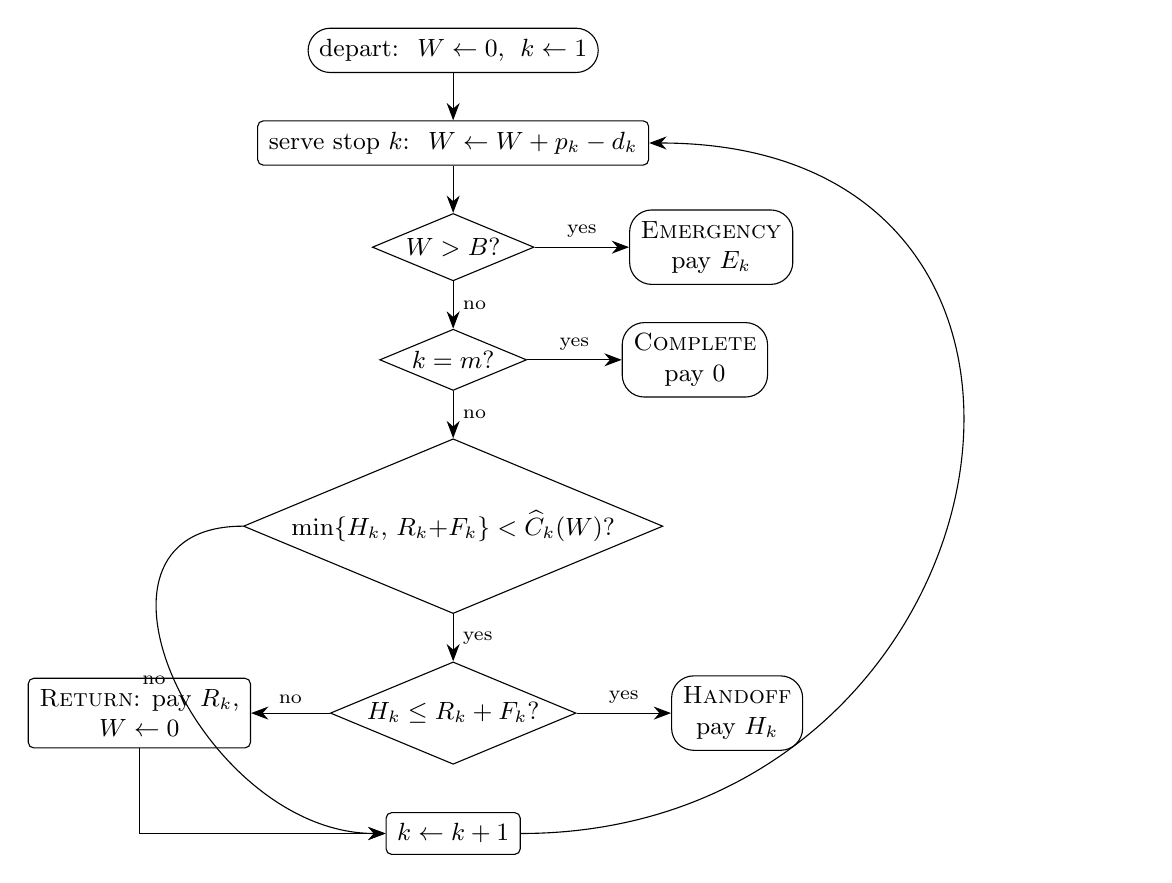
\begin{tikzpicture}[
  node distance=6mm and 8mm,
  box/.style={rectangle, rounded corners=2pt, draw, align=center,
              inner sep=4pt, font=\small},
  dec/.style={diamond, aspect=2.4, draw, align=center, inner sep=1.2pt,
              font=\small},
  term/.style={rectangle, rounded corners=8pt, draw, align=center,
               inner sep=4pt, font=\small},
  arr/.style={-{Stealth[length=2.2mm]}}]
\node[term] (start) {depart:\; $W \gets 0$,\; $k \gets 1$};
\node[box, below=of start] (serve)
  {serve stop $k$:\; $W \gets W + p_k - d_k$};
\node[dec, below=of serve] (guard) {$W > B$?};
\node[term, right=12mm of guard] (emg) {\textsc{Emergency}\\ pay $E_k$};
\node[dec, below=of guard] (last) {$k = m$?};
\node[term, right=12mm of last] (done) {\textsc{Complete}\\ pay $0$};
\node[dec, below=of last] (trig)
  {$\min\{H_k,\, R_k{+}F_k\} < \widehat C_k(W)$?};
\node[dec, below=of trig] (which) {$H_k \le R_k + F_k$?};
\node[term, right=12mm of which] (ho) {\textsc{Handoff}\\ pay $H_k$};
\node[box, left=10mm of which] (rs)
  {\textsc{Return}: pay $R_k$,\\ $W \gets 0$};
\node[box, below=of which] (inc) {$k \gets k + 1$};
\draw[arr] (start) -- (serve);
\draw[arr] (serve) -- (guard);
\draw[arr] (guard) -- node[above, font=\scriptsize]{yes} (emg);
\draw[arr] (guard) -- node[right, font=\scriptsize]{no} (last);
\draw[arr] (last) -- node[above, font=\scriptsize]{yes} (done);
\draw[arr] (last) -- node[right, font=\scriptsize]{no} (trig);
\draw[arr] (trig) -- node[right, font=\scriptsize]{yes} (which);
\draw[arr] (trig.west) to[out=180, in=180, looseness=1.4]
  node[left, font=\scriptsize]{no} (inc.west);
\draw[arr] (which) -- node[above, font=\scriptsize]{yes} (ho);
\draw[arr] (which) -- node[above, font=\scriptsize]{no} (rs);
\draw[arr] (rs) |- (inc);
\draw[arr] (inc.east) to[out=0, in=0, looseness=1.8] (serve.east);
\end{tikzpicture}%
}
\caption{Online decision loop of \textsc{Baton}. After every stop the
policy compares the estimated cost of continuing against the current
prices of the two recourse levers and exercises the cheaper lever only
when continuing is dearer; a depot return resets the load state and the
loop proceeds on the same route.}
\label{fig:flow}
\end{figure}

Three reference points calibrate the empirical results. The
\emph{clairvoyant bound} pays $0$ on $\{T = \infty\}$ and
$\min\{\min_{k<j} H_k,\, E_j\}$ on $\{T = j\}$---the cheapest of any
pre-breach handoff or the breach itself, with a breach at the first stop
leaving no decision epoch; no policy adapted to $(\mathcal F_k)$ that is
restricted to the handoff lever pays less on any path. Because it is
defined for the handoff lever, a policy with the richer menu may
legitimately beat it: a depot return costs less than a handoff and does
not end the route, so it can prevent a breach at a price no handoff-only
policy, clairvoyant or not, can match. When \textsc{Baton} exceeds this
bound, the excess measures the value of the second lever, not a
statistical artefact. The \emph{plug-in dynamic programs} replace the
isotonic step by quantile-binned conditional means. Run with fifty
times \textsc{Baton}'s training data they approach the exact solution
of the stopping problem in the $(k, W_k)$ state and serve as near-exact
yardsticks, one for the handoff-only problem (DP$_{50\mathrm{k}}$) and
one for the three-action problem (DP$^{3}_{50\mathrm{k}}$, whose
fresh-start values are computed on an independent half of the sample so
that they carry no in-sample optimism); at equal data the handoff-only
program is a fair equal-information competitor (DP$_N$). We emphasise a
point of method: mixed-integer programming, the exact technology of the
\emph{planning} stage, cannot compactly encode a non-anticipative
multistage stopping rule, so backward dynamic programming is the correct
exact anchor for the \emph{execution} stage; we use MIP where it
belongs, certifying the routing plans beneath all our experiments
(\S\ref{sec:large}).

Figures~\ref{fig:explainer} and~\ref{fig:explainer2} make the
machinery concrete on one route of the Hanoi instance introduced below:
the fan of simulated load paths with a demand-spike day highlighted, the
fitted continuation cost crossing the handoff price at stop 2---ten
stops before the breach the reactive policy suffers---and the resulting
expected cost over two thousand held-out days.

\begin{figure}[t]
\centering
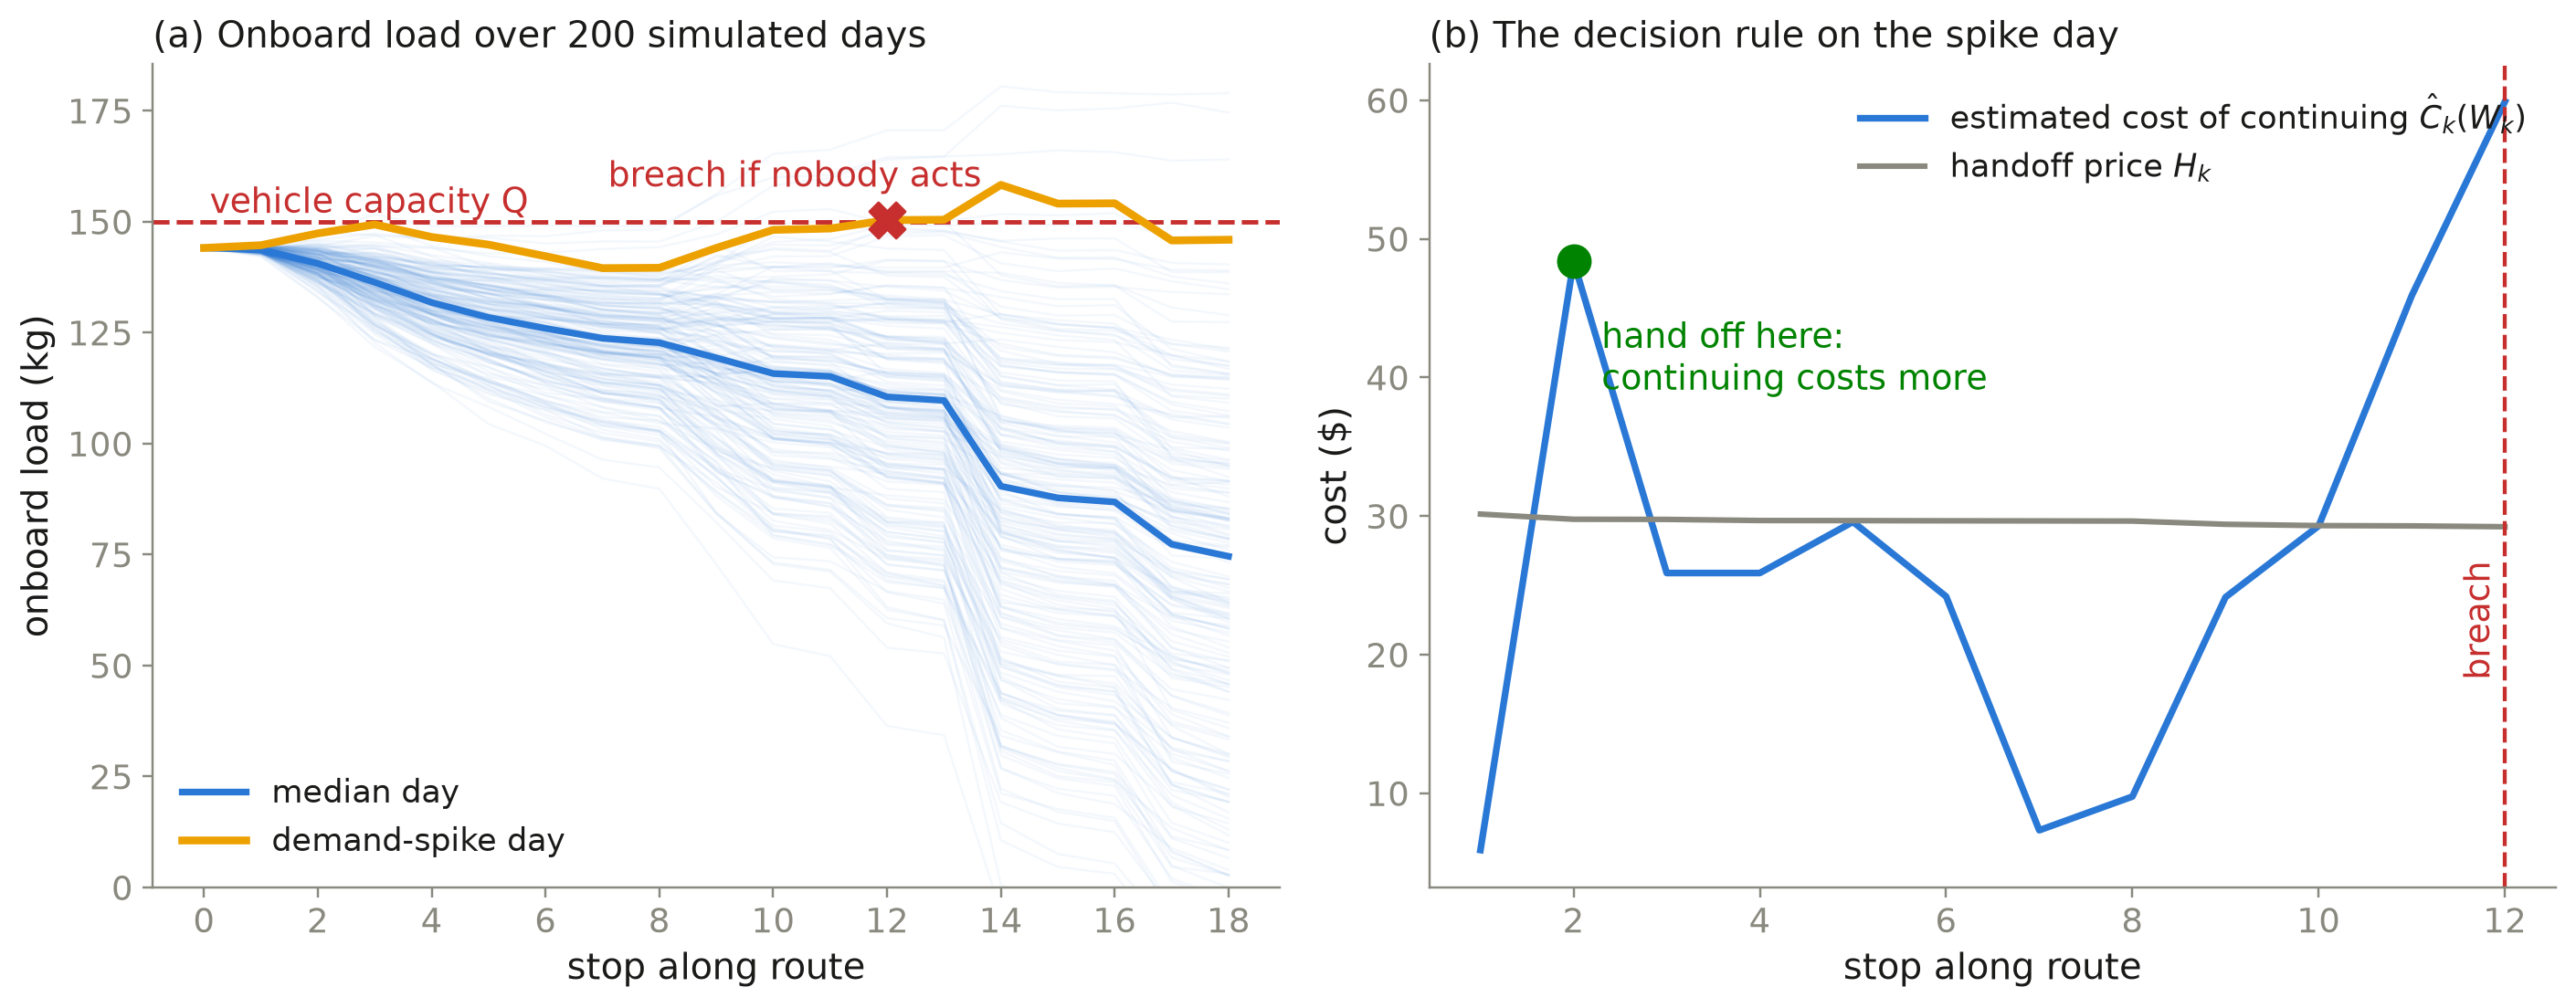
\includegraphics[width=\textwidth]{figures/fig2a_how_it_works}
\caption{\textsc{Baton} on one 18-stop route in Hanoi. (a) Onboard load
across 200 simulated days; the highlighted day breaches capacity at
stop 12 if nobody acts. (b) The decision rule on that day: the estimated
cost of continuing $\widehat C_k(W_k)$ crosses the per-stop handoff
price at stop 2, where the policy hands off.}
\label{fig:explainer}
\end{figure}

\begin{figure}[t]
\centering
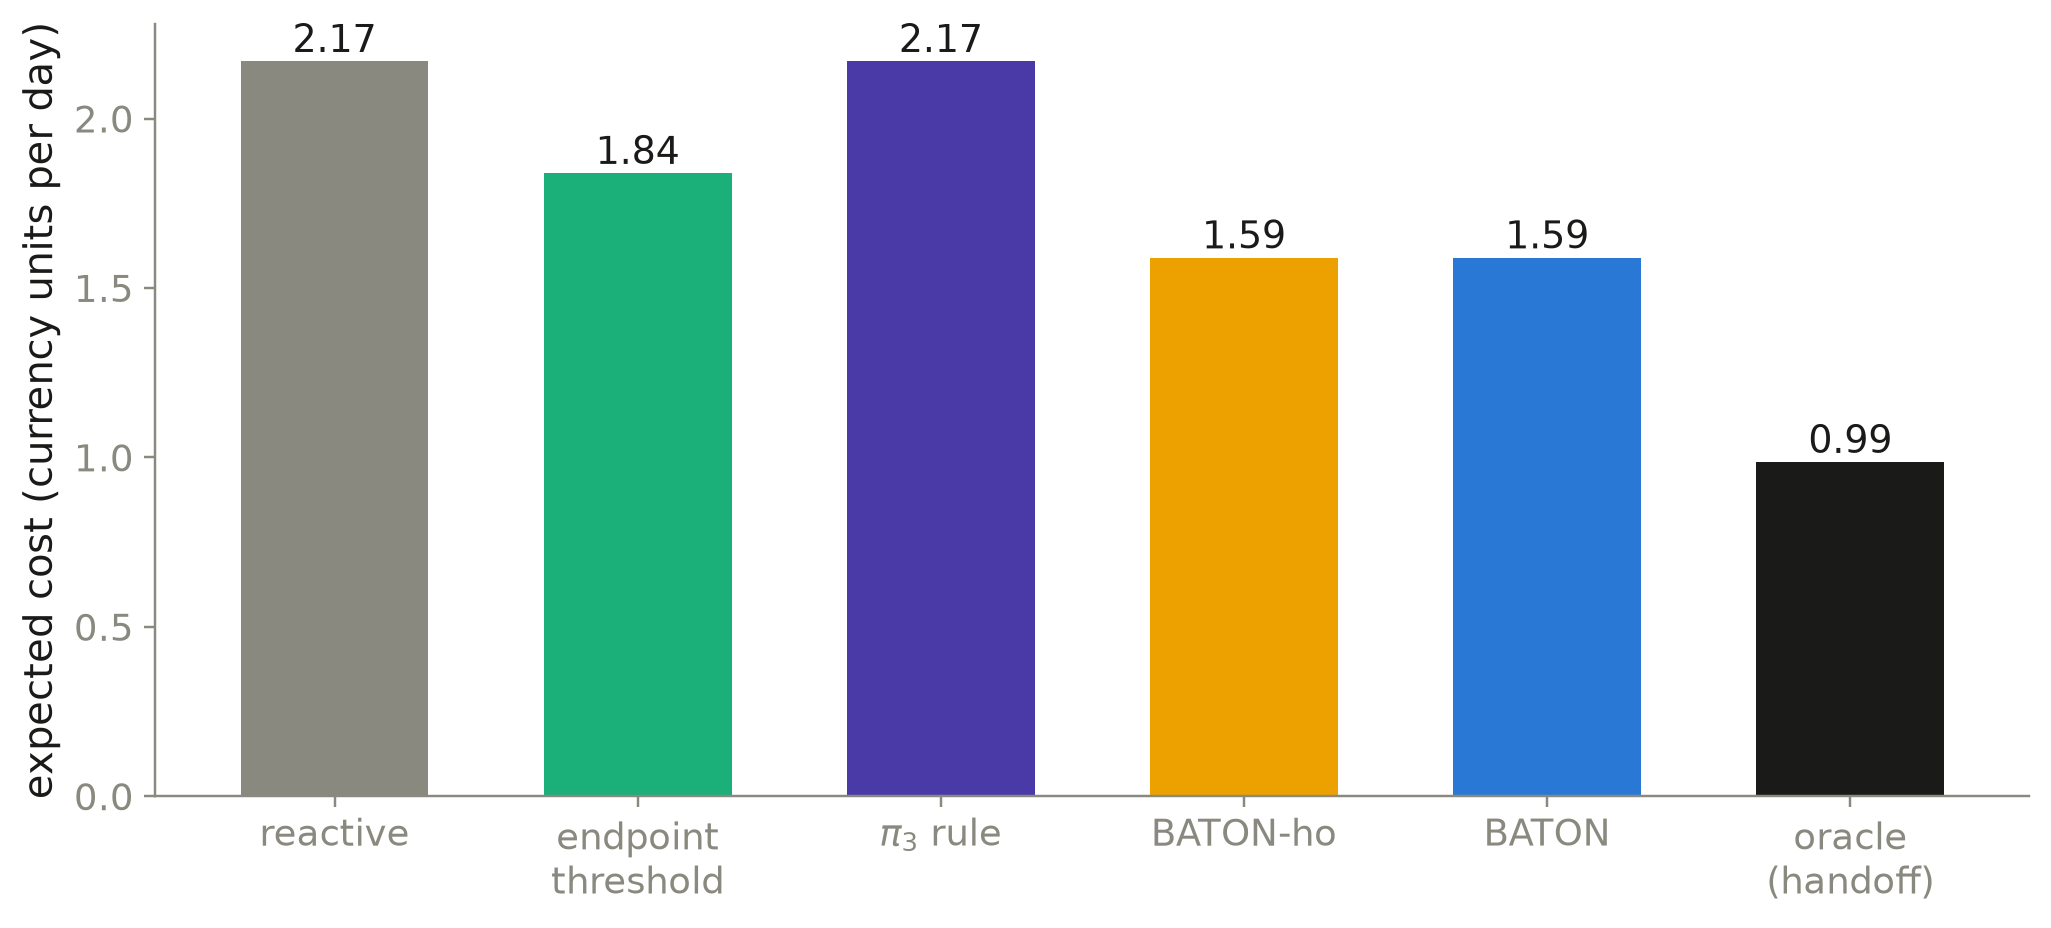
\includegraphics[width=0.78\textwidth]{figures/fig2b_test_costs}
\caption{Expected execution cost per policy on the route of
Figure~\ref{fig:explainer}, over 2{,}000 held-out days. On this route
deployment selection keeps the depot return switched off, so
\textsc{Baton} coincides with \textsc{Baton-ho}; the oracle is the
handoff-only clairvoyant bound.}
\label{fig:explainer2}
\end{figure}


% ══════════════════════════════════════════════════════════════════════
\section{Computational study}\label{sec:study}

Our computational study is designed around a simple discipline: every
claim about the policy must survive a change of environment, a change of
competitor, and a change of yardstick. This section first describes the
environments, competitors, and protocol (\S\ref{sec:setup}), then the
headline comparison across planning regimes with its statistical
analysis and tail risk (\S\ref{sec:headline}), the large-scale and
real-map benchmarks with the planning-stage certification
(\S\ref{sec:large}), the comparison against learning methods and the
empirical price of over-triggering (\S\ref{sec:learning}), the
robustness of the conclusions to the modelling assumptions
(\S\ref{sec:robust}), shared standby capacity (\S\ref{sec:pool}), data
and computing budgets (\S\ref{sec:budget}), and finally the economic and
spatial sensitivity analyses (\S\ref{sec:sensitivity}). All
experiments, result files, and figures are reproducible from a single
repository, and every table in this paper is generated mechanically from
the result files.

\subsection{Instances, planners, competitors, and protocol}
\label{sec:setup}

\paragraph{Instances} Three families are used. The 40 Dethloff
instances \citep{dethloff2001vehicle}, 50 customers each, are the
classical simultaneous pickup-and-delivery benchmark. The Salhi--Nagy
family \citep{salhi1999cluster}, 14 instances of 50--199 customers, is
derived from the CMT instances \citep{christofides1979vehicle} by the
standard coordinate-ratio demand split and extends the size range.
Finally, we introduce a set of instances built on the real drive
networks of Ho Chi Minh City, Hanoi, New York, Paris, and Shanghai
(6\,km radius around the centre, 5{,}800--15{,}800 road nodes per city):
customers are placed at \emph{real shop locations} drawn from
OpenStreetMap's retail layer, snapped to the nearest network node, so
the spatial demand distribution is the city's actual one---market
streets, malls, commercial clusters---and distances are true road
distances \citep{boeing2017osmnx}. Instance sizes reach 400 customers;
Figure~\ref{fig:cities} shows four of the instances with their planned
routes. Demands follow the benchmark protocol (gamma marginals,
coefficient of variation $0.3$, equicorrelated Gaussian copula
$\rho = 0.6$ among the deliveries and, independently, among the
pickups); the city instances use parcel-van magnitudes, with mean
deliveries of 8\,kg, pickup fractions uniform on $[0.2, 0.8]$, and
150\,kg vehicles, which yields the long 12--25-stop routes where
execution policy matters most. Because deliver-only customers are
common in practice, every city instance also has two deliver-only twins
in which the pickup of a random 25\% or 50\% of the customers is set to
zero; the twins are re-planned.

\begin{figure}[tp]
\centering
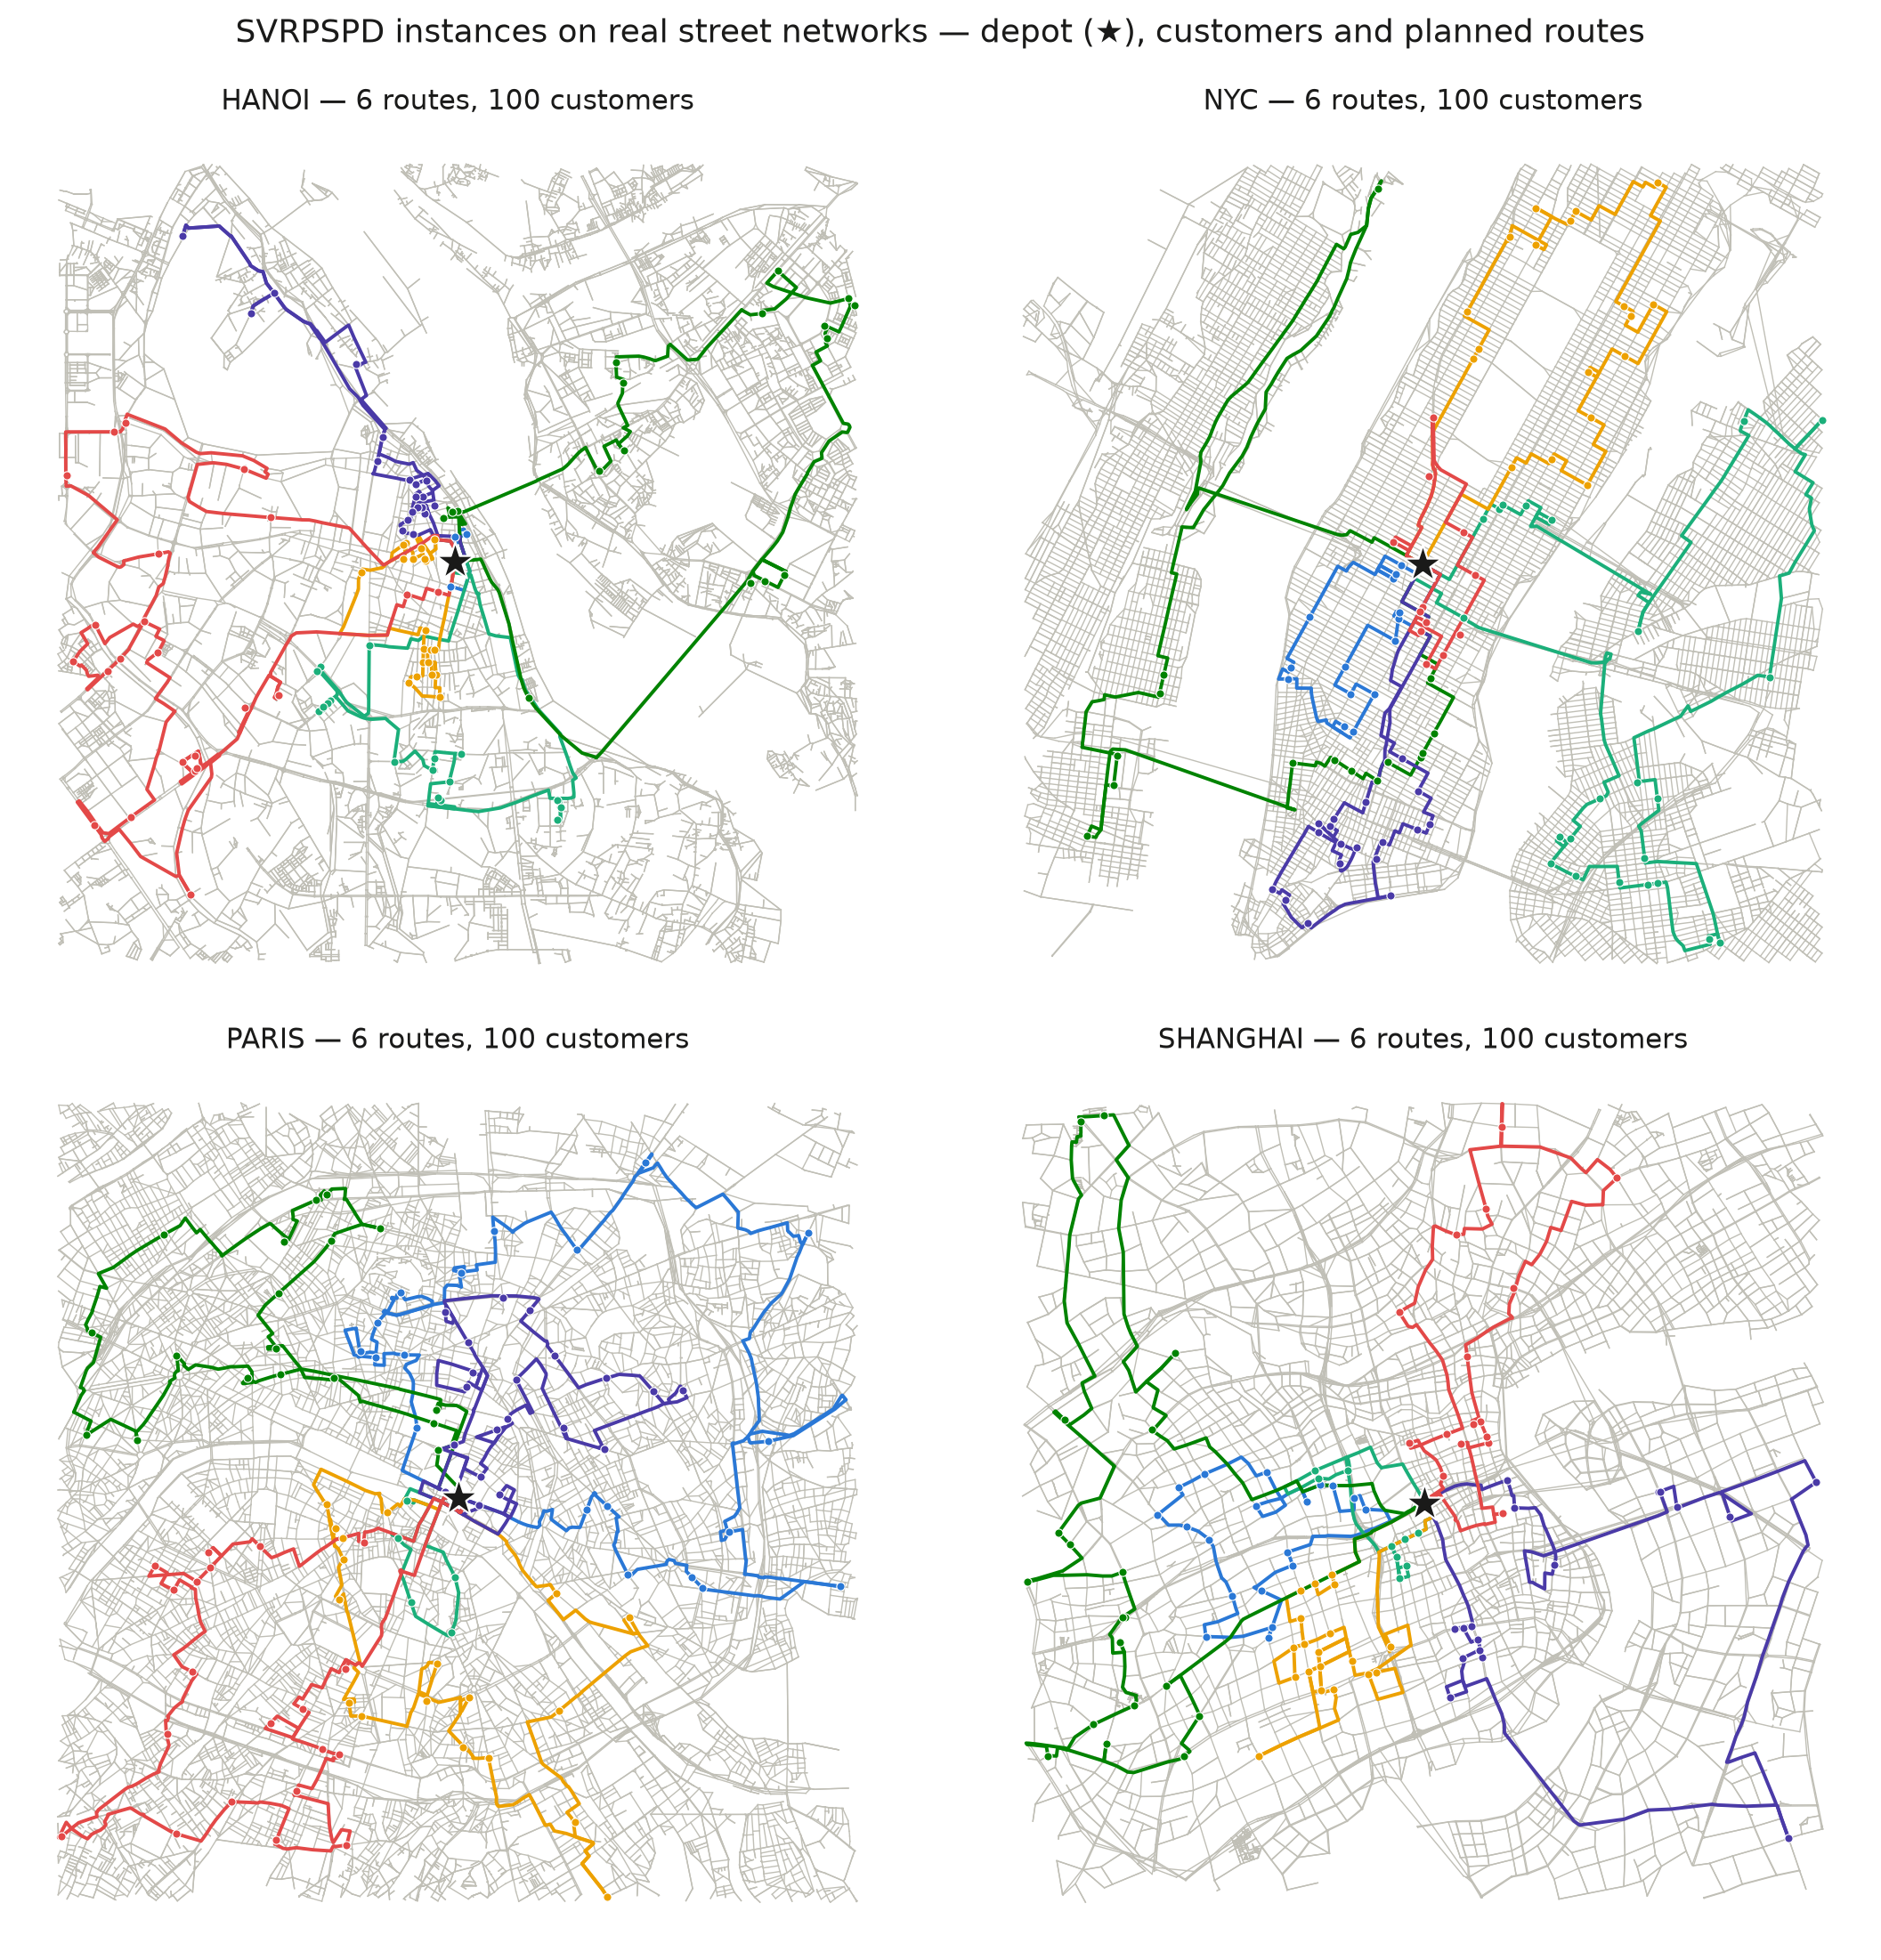
\includegraphics[width=\textwidth]{figures/fig1_city_maps}
\caption{City instances on real street networks, with customers at real
shop locations (Hanoi, New York, Paris, Shanghai; 100 customers each;
depot marked $\star$). Note the true retail clustering---Hanoi's Old
Quarter, Manhattan's commercial spine---that a uniform spatial
convention misses; \S\ref{sec:sensitivity} quantifies its effect.}
\label{fig:cities}
\end{figure}

\paragraph{Planning regimes} Routes are constructed by an adaptive
large neighbourhood search planner running under six capacity-feasibility
gates of increasing conservatism: a deterministic gate on the nominal
load peak (\textsc{Det}); a sample-average CVaR gate (\textsc{SAA}); a
Wasserstein distributionally robust gate (\textsc{WDRO})
\citep{esfahani2018data}; the quadrant-budget robust gate of
\citet{gounaris2013robust} (\textsc{Rob-G}); a budget-uncertainty gate
in the sense of \citet{bertsimas2004price} (\textsc{Rob-BS}); and a
moment-ambiguity gate in the closed form implied by
\citet{ghosal2024unifying} (\textsc{M-DRO}). With a type-1 Wasserstein
ball over unbounded support and a peak-load loss that is 1-Lipschitz,
the worst-case CVaR equals the empirical CVaR plus the constant
$\varepsilon/(1-\alpha)$ \citep{esfahani2018data}, so the
\textsc{WDRO} gate is the \textsc{SAA} gate at a tighter threshold; we
retain it as a distinct, more conservative planning regime rather than
as an independent modelling paradigm. Every execution policy is
evaluated on the identical plans of every gate, so planning quality
never contaminates the policy comparison; the plans themselves are
certified in \S\ref{sec:large}.

\paragraph{Competitors} Fourteen execution policies are compared, all
trained (where applicable) on scenarios strictly disjoint from the test
set: the \emph{reactive} policy that never intervenes; the incumbent
endpoint-labelled threshold and its myopic variant, retained as
ablations of Propositions~\ref{prop:bias} and \ref{prop:myopic}; the
\emph{label-corrected tuned threshold} (peak labels, one threshold tuned
on realised training cost); a \emph{position-dependent threshold} with
one load threshold per stop, tuned by coordinate descent on realised
training cost, which can represent any monotone stopping boundary and
therefore isolates the value of estimating that boundary by backward
induction rather than searching for it; the three published rule-based
restocking triggers $\pi_1, \pi_2, \pi_3$ of \citet{salavati2019rule},
adapted to the handoff lever and grid-tuned on realised cost; a
\emph{rollout} policy in the sense of \citet{secomandi2001rollout}, one
step of policy improvement over the reactive base---which, under
position-dependent prices, is exactly the myopic rule
$C^0_k(W_k) > H_k$---and a \emph{cost-scaled rollout} that hands off
when $C^0_k(W_k) > \theta H_k$ with $\theta$ tuned on realised cost; a
\emph{depot-return restocking} policy in the tradition of
\citet{yang2000stochastic} and \citet{florio2020new}, with real detour
prices and a tuned trigger; \textsc{Baton-ho}, the handoff-only
restriction of our policy; \textsc{Baton} itself; and the equal-data
plug-in dynamic program DP$_{N}$. \textsc{Baton-cf}, the variant with a
state-conditional fresh-start value, is reported in \S\ref{sec:robust}.
A reinforcement-learning policy re-implemented from
\citet{iklassov2024rl} is compared separately in \S\ref{sec:learning}.
The two near-exact programs DP$_{50\mathrm{k}}$ and DP$^3_{50\mathrm{k}}$
and the clairvoyant bound close every table as reference points.
Table~\ref{tab:competitors} collects the roster with sources; in every
results table the reported quantity is the expected-recourse saving
relative to the reactive policy, in percent, so \emph{higher is always
better}.

\begin{table}[tp]
\caption{Execution policies compared in this paper. Policies marked
``tuned'' receive their best hyper-parameter(s) by search on realised
cost over the training scenarios; \textsc{Baton} has no tunable
parameter. The last three rows are reference points, not competitors.}
\label{tab:competitors}
\centering
\small
\setlength{\tabcolsep}{4pt}
\begin{tabular}{l p{5.3cm} p{4.4cm}}
\toprule
Label & Policy & Source \\
\midrule
reactive & never intervenes; emergency on breach & baseline \\
endpoint $+\,\tau$ & endpoint-label threshold (tuned), and its
  myopic variant & ablation (Props.~\ref{prop:bias}, \ref{prop:myopic}) \\
thr. & peak-label threshold (tuned) & threshold ablation \\
thr.-$k$ & one load threshold per stop (tuned by coordinate descent) &
  position-dependent threshold \\
$\pi_1$--$\pi_3$ & rule-based restocking triggers (tuned) &
  \citet{salavati2019rule} \\
roll. & one-step policy improvement (myopic cost rule) &
  \citet{secomandi2001rollout} \\
roll.-$\theta$ & myopic cost rule with tuned price multiplier &
  cost-dependent threshold \\
restock & depot-return restocking, tuned trigger &
  \citet{yang2000stochastic}; \citet{florio2020new} \\
RL & policy-gradient network &
  \citet{iklassov2024rl} \\
DP$_N$ & plug-in dynamic program, equal data &
  \citet{secomandi2009reoptimization} \\
\textsc{Baton-ho} & handoff-only restriction of our policy & this paper \\
\textsc{Baton} & priced-action optimal stopping & this paper \\
\textsc{Baton-cf} & \textsc{Baton} with state-conditional fresh-start
  value & this paper \\
\midrule
DP$_{50\mathrm{k}}$, DP$^3_{50\mathrm{k}}$ & plug-in dynamic program,
  $50{\times}$ data, handoff-only / three actions & near-exact reference \\
oracle & clairvoyant per-day optimum (handoff-only) & bound \\
\bottomrule
\end{tabular}
\end{table}

\paragraph{Protocol} For each instance, one set of $10^3$ training
days, one set of $2 \times 10^3$ test days and one set of
$5 \times 10^4$ reference days are drawn from independent random
streams whose seeds are fixed functions of the instance name, so every
run of the pipeline draws identical scenarios. All routes of a plan
share the same days, as they would in operation. Every data-driven
policy---\textsc{Baton}, the thresholds, the rule-based triggers, the
rollouts, the restocking trigger, DP$_N$ and the RL policy---sees
exactly the same $10^3$ training days; hyper-parameters of the tuned
competitors are selected on realised cost over those same training days
(there is no separate validation set, which, if anything, favours the
tuned competitors: \textsc{Baton} has nothing to tune). The test days
are used only for the reported evaluation. The reference programs use
the $5 \times 10^4$ reference days; DP$^3_{50\mathrm{k}}$ fits on one
half and values its fresh-start states on the other. Offline fitting
time and online decision time are reported separately in
\S\ref{sec:budget}.

\paragraph{Statistical analysis} The experimental unit is the instance
within a planning gate: policies are compared on the plan-level expected
recourse cost, the sum over the plan's routes of the mean over the
$2 \times 10^3$ test days. Routes of a plan share their test days and
are therefore not treated as independent observations, and the six
gates re-use the same forty instances, so we analyse each gate
separately ($n = 40$) rather than pooling them. For each comparison we
report the mean paired difference in saving with a 95\% bootstrap
confidence interval, the number of instances won, the matched-pairs
rank-biserial effect size, and a two-sided Wilcoxon signed-rank test
with Holm's correction across all comparisons of a table. Route-level
results for every policy, gate and instance are provided as
supplementary data, and the tail of the daily plan-level bill is
analysed separately.

\paragraph{Fleet economics} The defaults are
$F_{\mathrm{plan}} = 35$, $F_{\mathrm{sb}} = 20$,
$F_{\mathrm{ho}} = 5$, $c_{\mathrm{tr}} = 3$, $F_{\mathrm{emg}} = 40$,
$s_{\mathrm{ho}} = 1.2$, $s_{\mathrm{emg}} = 2.5$,
$p_{\mathrm{late}} = 1.5$, $p_{\mathrm{breach}} = 10$ (currency units
per vehicle-day or per event; kilometre costs $c_{\mathrm{km}} = 0.1$),
calibrated to the order of magnitude of Southeast-Asian gig-logistics
rates and swept in \S\ref{sec:sensitivity}.

\paragraph{Software} All planning and execution code is Python 3.11.15
(NumPy 2.4.6, SciPy 1.17.1, pandas 3.0.3); the isotonic regressions of
Algorithm~\ref{alg:offline} use scikit-learn 1.9.1. The MIP
certification of \S\ref{sec:large} solves the two-commodity flow
formulation through PuLP 3.3.2 with Gurobi 13.0.2 as the primary solver
and the open-source HiGHS 1.15.1 as an independent cross-check; both
solvers run single-model with a 300-second budget per instance and
default tolerances. Street networks and shop locations come from
OpenStreetMap via OSMnx 2.1.0 \citep{boeing2017osmnx}, and the
reinforcement-learning baseline is trained with PyTorch 2.14 on the same
CPU. Everything else---the ALNS planner, all six gates, and every
execution policy of Table~\ref{tab:competitors}---is implemented from
the cited papers in plain Python within our repository, so all
competitors share the same simulator, cost model, and data.

\subsection{Headline comparison across planning regimes}
\label{sec:headline}

Table~\ref{tab:grand} reports the central result, Figure~\ref{fig:gatedots}
draws it, and Table~\ref{tab:stats} gives the paired statistics. Four
observations organise the discussion.

\begin{table}[t]
\caption{Expected-recourse saving over the reactive policy (\%, mean over
the 40 Dethloff instances) for each planning gate and execution policy
under the three-class fleet cost model; \emph{higher is better}.
\textsc{Baton} (bold) has the highest saving of all implementable
policies on every gate. thr.\ is the label-corrected tuned threshold,
thr.-$k$ the position-dependent threshold, roll.-$\theta$ the
cost-scaled rollout. The last three columns are reference points, not
competitors: DP$_{50\mathrm{k}}$ and DP$^3_{50\mathrm{k}}$ are
near-exact dynamic programs for the handoff-only and the three-action
problem with fifty times the training data, and the clairvoyant oracle
is restricted to the handoff lever, so \textsc{Baton} may legitimately
exceed it.}
\label{tab:grand}
\centering
\footnotesize
\setlength{\tabcolsep}{2.6pt}
\begin{adjustbox}{max width=\textwidth}
\begin{tabular}{l cccccc cc ccc}
\toprule
& \multicolumn{6}{c}{published / tuned competitors}
& \multicolumn{2}{c}{this paper} & \multicolumn{3}{c}{reference points} \\
\cmidrule(lr){2-7}\cmidrule(lr){8-9}\cmidrule(lr){10-12}
Gate & $\pi_3$ & roll. & roll.-$\theta$ & restock & thr. & thr.-$k$ & \textsc{Baton-ho} & \textsc{Baton} & DP$_{50\mathrm{k}}$ & DP$^3_{50\mathrm{k}}$ & oracle \\
\midrule
\textsc{Det} & 17.0 & 20.8 & 24.9 & 5.8 & 24.7 & 25.8 & 26.1 & \textbf{27.9} & 26.4 & 29.5 & 40.7 \\
\textsc{SAA} & 12.6 & 8.9 & 18.4 & 43.7 & 16.3 & 15.4 & 20.1 & \textbf{53.7} & 22.1 & 56.4 & 43.5 \\
\textsc{WDRO} & 8.0 & -4.2 & 8.9 & 34.7 & -1.3 & -0.2 & 10.0 & \textbf{41.2} & 13.2 & 47.8 & 42.0 \\
\textsc{Rob-G} & 15.7 & 10.1 & 19.1 & 43.6 & 16.7 & 16.7 & 21.0 & \textbf{53.2} & 22.9 & 56.3 & 43.3 \\
\textsc{Rob-BS} & 11.1 & 10.3 & 18.7 & 42.0 & 16.7 & 16.3 & 20.7 & \textbf{52.5} & 22.6 & 54.9 & 43.1 \\
\textsc{M-DRO} & 9.6 & -1.4 & 10.3 & 37.4 & 0.5 & -1.0 & 11.8 & \textbf{45.3} & 14.2 & 50.2 & 42.2 \\
\bottomrule
\end{tabular}
\end{adjustbox}
\end{table}


\begin{figure}[t]
\centering
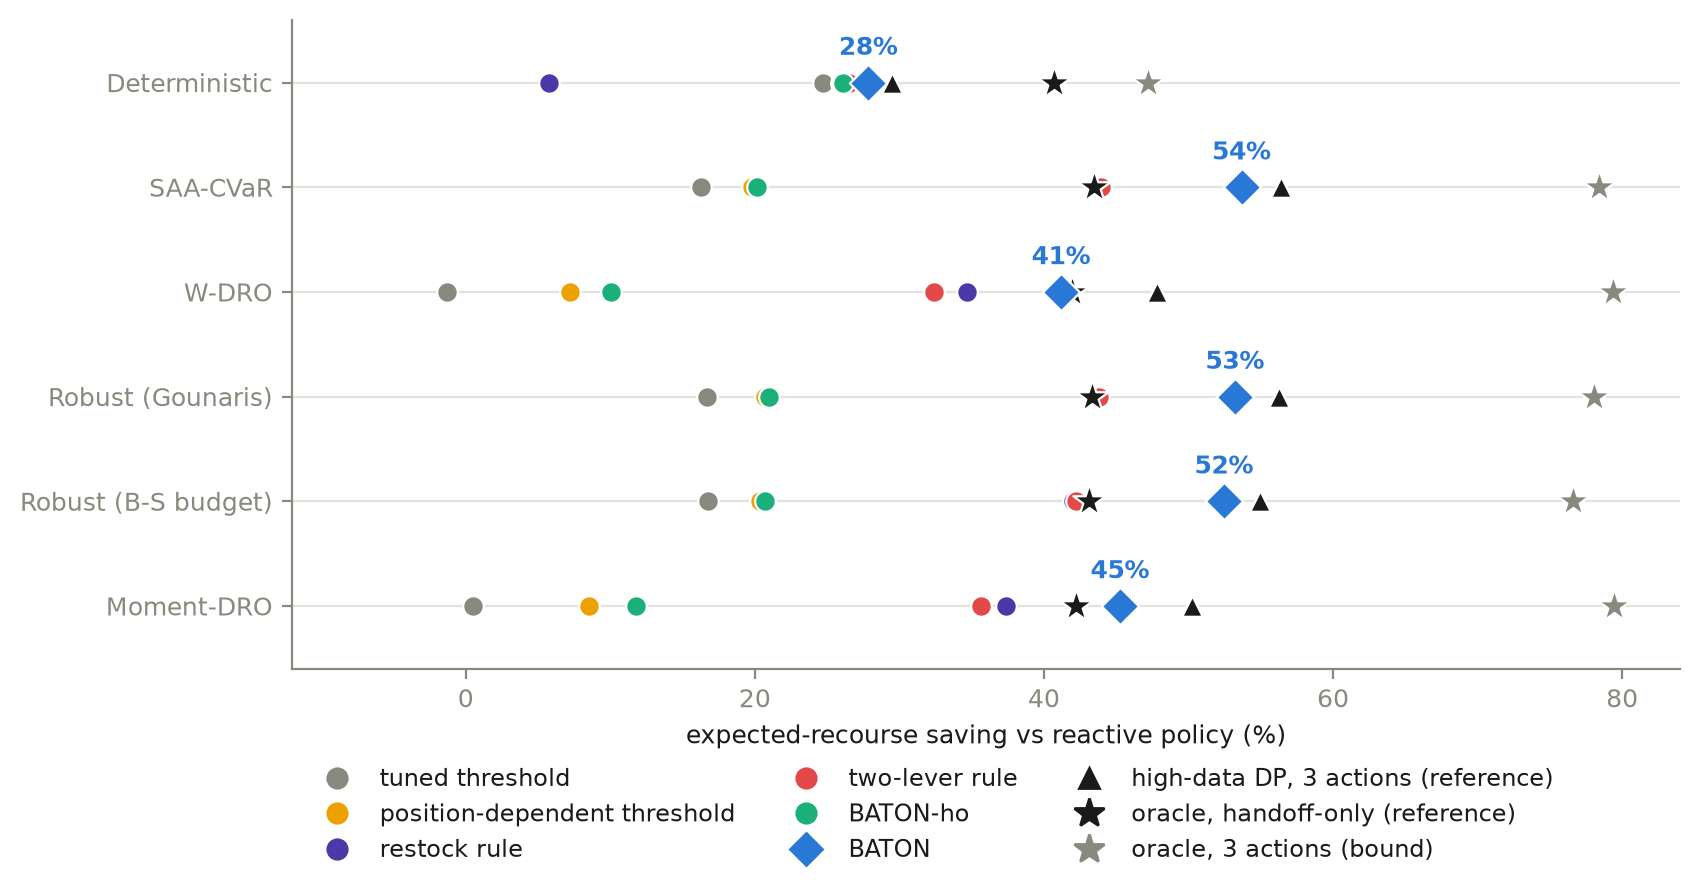
\includegraphics[width=\textwidth]{figures/fig4_gate_dots}
\caption{Expected-recourse saving by planning gate and execution policy
(Table~\ref{tab:grand} drawn). \textsc{Baton} (diamonds) leads the
implementable policies on every gate and exceeds the handoff-only
clairvoyant bound (stars) wherever plans leave slack for the
depot-return lever to work with.}
\label{fig:gatedots}
\end{figure}

\begin{table}[t]
\caption{Paired comparison of \textsc{Baton} with, in turn, the strongest
competitor on each gate, its handoff-only restriction, and the high-data
three-action reference program. The strongest competitor is not fixed in
advance: it is the implementable policy other than the \textsc{Baton}
variants with the highest mean saving among the ten competitors of
Table~\ref{tab:competitors} that were run on all gates. Because it is
selected on the same instances, its interval re-selects the competitor
in every bootstrap resample, and its $p$-value is the largest of the
Wilcoxon $p$-values against the ten competitors taken one at a time (an
intersection-union test of ``better than every competitor'', valid
without a selection correction). The experimental unit is the
instance ($n = 40$ per gate; the routes of a plan share their test days
and are aggregated within the plan). $\Delta$: mean difference in saving
(percentage points; positive favours \textsc{Baton}) with a 95\%
bootstrap confidence interval; W: instances on which \textsc{Baton} is
better; $r$: matched-pairs rank-biserial effect size; $p$: two-sided
Wilcoxon signed-rank test, Holm-adjusted over the 18 comparisons.}
\label{tab:stats}
\centering
\scriptsize
\setlength{\tabcolsep}{2.2pt}
\begin{adjustbox}{max width=\linewidth}
\begin{tabular}{l l cccc cccc cccc}
\toprule
& & \multicolumn{4}{c}{vs.\ strongest competitor}
& \multicolumn{4}{c}{vs.\ \textsc{Baton-ho}}
& \multicolumn{4}{c}{vs.\ DP$^3_{50\mathrm{k}}$ (reference)} \\
\cmidrule(lr){3-6}\cmidrule(lr){7-10}\cmidrule(lr){11-14}
Gate & competitor & $\Delta$ [95\% CI] & W & $r$ & $p$
& $\Delta$ [95\% CI] & W & $r$ & $p$ & $\Delta$ [95\% CI] & W & $r$ & $p$ \\
\midrule
\textsc{Det} & DP$^3_N$ & +0.0 [-0.4, +0.4] & 21 & +0.13 & 0.489 & +1.8 [+1.4, +2.2] & 40 & +1.00 & $<\!10^{-4}$ & -1.6 [-2.2, -1.2] & 0 & -1.00 & $<\!10^{-4}$ \\
\textsc{SAA} & two-lever & +9.7 [+8.2, +11.1] & 40 & +1.00 & $<\!10^{-4}$ & +33.5 [+32.0, +35.0] & 40 & +1.00 & $<\!10^{-4}$ & -2.7 [-3.3, -2.2] & 0 & -1.00 & $<\!10^{-4}$ \\
\textsc{WDRO} & restock & +6.5 [+3.6, +9.7] & 31 & +0.70 & $<\!10^{-3}$ & +31.2 [+28.6, +33.7] & 40 & +1.00 & $<\!10^{-4}$ & -6.6 [-8.9, -4.6] & 3 & -0.91 & $<\!10^{-4}$ \\
\textsc{Rob-G} & two-lever & +9.4 [+7.7, +10.9] & 40 & +1.00 & $<\!10^{-4}$ & +32.3 [+30.5, +33.9] & 40 & +1.00 & $<\!10^{-4}$ & -3.1 [-3.6, -2.6] & 1 & -1.00 & $<\!10^{-4}$ \\
\textsc{Rob-BS} & two-lever & +10.3 [+8.1, +12.3] & 40 & +1.00 & $<\!10^{-4}$ & +31.8 [+30.3, +33.2] & 40 & +1.00 & $<\!10^{-4}$ & -2.5 [-2.9, -2.0] & 2 & -0.99 & $<\!10^{-4}$ \\
\textsc{M-DRO} & restock & +7.9 [+5.1, +11.1] & 34 & +0.89 & $<\!10^{-4}$ & +33.5 [+30.9, +36.1] & 40 & +1.00 & $<\!10^{-4}$ & -5.0 [-7.2, -3.1] & 5 & -0.84 & $<\!10^{-4}$ \\
\bottomrule
\end{tabular}
\end{adjustbox}
\end{table}


First, \textsc{Baton} has the highest saving of every implementable
policy on every gate. Against the strongest competitor of each
gate---the position-dependent threshold on \textsc{Det}, depot-return
restocking on the five conservative gates---its mean advantage ranges
from \statCompDeltaMin{} to \statCompDeltaMax{} percentage points; the
95\% confidence interval excludes zero on every gate, \textsc{Baton} is
better on at least \statCompWinMin{} of the 40 instances, and
\statPmax{} throughout. Against the near-exact three-action program,
which sees fifty times its data, \textsc{Baton} attains
\ratioDpThreeLo--\ratioDpThreeHi{} of its saving; the shortfall is the
finite-sample price of learning from a thousand days, and
\S\ref{sec:budget} shows that it closes as the history grows.

Second, the \emph{composition} of the win changes across gates in an
instructive way. On the deterministic gate, routes depart packed to
capacity, most breach risk sits at the first stop where no online
policy can act, and all preventive policies compress toward each other;
\textsc{Baton}'s margin there (\svDetBaton{} against \svDetThresh{} for
the tuned threshold) comes mostly from the trigger correction of
Proposition~\ref{prop:myopic}. On every conservative gate---the two
sample-based gates and all three published robust planners---plans
carry slack, breaches happen mid-route, and the depot-return lever
becomes live: \textsc{Baton} more than doubles the saving of the best
handoff-only policy (for instance \svSAABaton{} against \svSAAHo{} on
\textsc{SAA} plans) and exceeds the handoff-only clairvoyant bound
(\svSAAOrc{}) on \nOrcBeat{} of the six gates. As explained in
\S\ref{sec:algorithms}, that bound is clairvoyant only about the
handoff lever: beating it is not a paradox but a measurement of how
much the second lever is worth when priced optimally.

Third, richer threshold classes do not rescue the threshold family. On
\textsc{WDRO} and \textsc{M-DRO} plans the tuned threshold's saving is
negative or negligible (\svWDROThresh{} and \svMDROThresh{}): with
handoffs carrying their true standby cost, its interventions cost about
as much as they prevent. The position-dependent threshold, which can
represent any monotone stopping boundary, does no better
(\svWDROThrK{} on \textsc{WDRO}); searching $m-1$ boundaries directly
against realised cost on a thousand days has more variance than
estimating them by backward induction, and on \textsc{Det} plans, where
it is strongest, it still trails \textsc{Baton-ho} (\svDetThrK{}
against \svDetHo{}). The cost-scaled rollout, a threshold on the myopic
cost with a tuned price multiplier, is the best handoff-only
competitor on the conservative gates but stays below
\textsc{Baton-ho} everywhere. A policy that prices actions declines to
act when acting has negative value; a policy that memorises a trigger
level, however flexibly, has to learn that boundary from realised cost
alone.

Fourth, the gains extend to the tail. Table~\ref{tab:tail} reports the
mean of the worst 5\% of daily plan-level bills and the probability that
at least one route of a plan suffers an emergency on a given day.
\textsc{Baton} cuts the CVaR$_{95}$ of the daily bill by
\tailBatonLo--\tailBatonHi{} relative to the reactive policy and, on the
conservative gates, lowers the daily emergency probability more than
any handoff-only policy, because a depot return prevents breaches that a
priced handoff would not be worth. On \textsc{Det} plans the emergency
probability of all policies stays high, again because the risk sits at
the first stop.

\begin{table}[t]
\caption{Tail risk of the daily recourse bill of a plan (40 Dethloff
instances per gate, 2{,}000 test days each). CVaR$_{95}$: mean of the
worst 5\% of daily plan bills; the reactive column gives its level in
currency units, the others its reduction (\%, higher is better).
$P(\mathrm{emg})$: share of days on which at least one route of the plan
suffers an emergency (\%, lower is better).}
\label{tab:tail}
\centering
\footnotesize
\setlength{\tabcolsep}{3.5pt}
\begin{tabular}{l c ccc cccc}
\toprule
& \multicolumn{4}{c}{CVaR$_{95}$ of daily plan bill} &
\multicolumn{4}{c}{$P(\mathrm{emg})$ per day (\%)} \\
\cmidrule(lr){2-5}\cmidrule(lr){6-9}
Gate & reactive & thr. & \textsc{Baton-ho} & \textsc{Baton} &
reactive & thr. & \textsc{Baton-ho} & \textsc{Baton} \\
\midrule
\textsc{Det} & 481.5 & 23.6 & 23.8 & \textbf{22.3} & 61.7 & 43.5 & 41.4 & \textbf{41.4} \\
\textsc{SAA} & 256.0 & 20.1 & 22.2 & \textbf{54.3} & 10.0 & 6.6 & 6.4 & \textbf{4.3} \\
\textsc{WDRO} & 58.9 & 1.3 & 7.2 & \textbf{37.9} & 2.3 & 1.6 & 1.7 & \textbf{1.3} \\
\textsc{Rob-G} & 280.2 & 21.3 & 23.2 & \textbf{52.2} & 11.3 & 7.7 & 7.6 & \textbf{5.2} \\
\textsc{Rob-BS} & 302.7 & 21.1 & 22.9 & \textbf{52.0} & 11.6 & 8.3 & 8.1 & \textbf{5.6} \\
\textsc{M-DRO} & 72.2 & 3.0 & 9.3 & \textbf{42.4} & 2.7 & 1.9 & 2.0 & \textbf{1.4} \\
\bottomrule
\end{tabular}
\end{table}


The synthetic scenarios of Table~\ref{tab:synthetic} isolate the two
defects of \S\ref{sec:defects} under controlled conditions and confirm
Proposition~\ref{prop:bias} at its extremal point: on
collect-then-deliver structure the endpoint-trained policy saves
exactly \ctdVOne{}---it never intervenes---while the label-corrected
policies save about half of the reactive cost, the option-value
correction adds a further margin that grows with route length and the
price ratio, and a depot return (priced flat at half a handoff) lifts
\textsc{Baton} to \ctdBatonFull{}.

\begin{table}[t]
\caption{Structural synthetic scenarios (five seeds, $1.2\times10^4$ test
routes each, flat prices $\omega_F = 1$, $C_{\mathrm{fail}}/\omega_F$
as shown or 5): saving \% over the reactive policy, \emph{higher is
better}. The synthetic routes have no geometry, so the depot return of
the full \textsc{Baton} is priced flat at half a handoff; the first
three columns use the handoff lever only. On collect-then-deliver
structure the endpoint-labelled predecessor never intervenes.}
\label{tab:synthetic}
\centering
\begin{adjustbox}{max width=\linewidth}
\begin{tabular}{l cccc}
\toprule
Scenario & endpoint + $\tau$ & peak + $\tau$ & \textsc{Baton-ho} &
\textsc{Baton} \\
\midrule
collect-then-deliver & 0.0 & 49.2 & 51.9 & \textbf{69.1} \\
milk run, regime switching & 58.9 & 58.9 & 63.8 & \textbf{78.5} \\
milk run, $C/\omega = 20$ & 85.5 & 85.5 & 88.2 & \textbf{93.5} \\
\bottomrule
\end{tabular}
\end{adjustbox}
\end{table}


\subsection{Scale, real maps, and certified plans}\label{sec:large}

Table~\ref{tab:large} extends the comparison to the Salhi--Nagy family
and the city instances. On Salhi--Nagy, whose 50--199-customer routes
are tight and long, the picture of the conservative Dethloff gates
repeats at scale: \textsc{Baton} saves \svSalhiBaton{} of reactive
cost---against \svSalhiHo{} for its handoff-only restriction and beyond
the handoff-only oracle (\svSalhiOrc{})---with the depot-return lever
doing heavy work on the centrally located depots of the CMT geometry.

On the city instances the same policy correctly reverses itself. Real
urban depots sit at the retail centre of gravity, but detours through
congested networks are long and the delivery-dominated routes rarely
come close to capacity late in the day, so the return lever rarely pays.
Deployment selection keeps it in the menu on only \cityActShare{} of the
routes, and \textsc{Baton} equals its handoff-only restriction
(\svCityBaton{} against \svCityHo{} across \nCity{} instances) rather
than paying the estimation cost of a useless action. The three-action
policy's value is therefore concentrated in settings with central depots
and slack plans; on the dense urban networks we studied, the handoff
lever does the work. Two reference points lie above \textsc{Baton} on
the city instances, and neither is a competitor. The oracle knows the
day's demands in advance; on city routes much of the breach risk comes
from demand surprises at the next stop that no policy observing only the
past can anticipate, which is why its lead is large (\svCityOrc{}).
DP$_{50\mathrm{k}}$ is fitted on fifty times more data. With the return
lever idle, the gap between it and \textsc{Baton} (\svCityDp{} against
\svCityBaton{}) is the finite-sample cost of estimating the stopping
boundary from $10^3$ days, and \S\ref{sec:budget} shows it closing as
the history grows. The uniform-scatter twins behave the same way.

The deliver-only twins test a feature of real demand that the benchmark
protocol lacks. With a quarter or a half of the customers collecting
nothing, the load rises less along the route, breaches become rarer,
and every policy has less to save. \textsc{Baton} still saves
\svZpTwentyFiveBaton{} and \svZpFiftyBaton{}, while the tuned threshold
falls to \svZpFiftyThr{} at 50\% deliver-only customers. In this
setting, where recourse is worth least, the position-dependent threshold
matches \textsc{Baton} within a few tenths of a point.

\begin{sidewaystable}
\caption{Large-scale benchmarks under the fleet cost model
(\textsc{Det}-gate plans unless stated; saving \% vs.\ reactive,
\emph{higher is better}; the best implementable policy of each row is in
bold; columns as in Table~\ref{tab:grand}, the four columns after
\textsc{Baton-cf} being reference points). Salhi--Nagy instances carry
50--199 customers; the city instances (100--400 customers) place
customers at real OSM shop locations on the road networks of Ho Chi Minh
City, Hanoi, New York, Paris and Shanghai. The uniform twins use the
same cities and demands with uniformly scattered customers; the
deliver-only twins set the pickup of a random 25\% or 50\% of the
customers to zero and are re-planned. Last column: \textsc{Baton} minus
the strongest competitor of the row (named), mean over instances in
percentage points with a 95\% paired bootstrap interval that re-selects
the strongest competitor in every resample.}
\label{tab:large}
\centering
\small
\setlength{\tabcolsep}{3pt}
\begin{adjustbox}{max width=\linewidth}
\begin{tabular}{l r cccccc ccc cccc l}
\toprule
Benchmark & $n$ & restock & thr. & thr.-$k$ & two-lever & DP$_N$ & DP$^3_N$ &
\textsc{Baton-ho} & \textsc{Baton} & \textsc{Baton-cf} &
DP$_{50\mathrm{k}}$ & DP$^3_{50\mathrm{k}}$ & oracle-ho & oracle$^3$ &
$\Delta$ vs.\ best competitor \\
\midrule
Salhi--Nagy & 14 & 26.5 & 37.4 & 42.2 & 45.2 & 41.9 & 52.3 & 42.3 & 53.0 & \textbf{53.6} & 42.8 & 54.0 & 48.8 & 62.2 & +0.7 [+0.2, +1.2] (DP$^3_N$) \\
City, real shops & 19 & 0.3 & 9.7 & 10.1 & 10.0 & 6.8 & 3.4 & 10.6 & 10.6 & \textbf{10.8} & 12.1 & 12.3 & 36.8 & 37.7 & +0.5 [+0.05, +0.68] (thr.-$k$) \\
City, uniform & 9 & 0.1 & 11.7 & 11.3 & 11.5 & 8.5 & 5.3 & 11.7 & 11.8 & \textbf{12.1} & 12.9 & 13.1 & 35.2 & 36.4 & +0.1 [-0.8, +0.6] (roll.-$\theta$) \\
City, 25\% deliver-only & 19 & -0.3 & 3.7 & 4.5 & 3.8 & 1.9 & 1.7 & 4.8 & 4.9 & \textbf{5.0} & 6.2 & 6.4 & 32.1 & 32.7 & +0.4 [+0.03, +0.61] (thr.-$k$) \\
City, 50\% deliver-only & 19 & -0.5 & -1.5 & 0.1 & 1.8 & \textbf{3.1} & 2.1 & \textbf{3.1} & \textbf{3.1} & \textbf{3.1} & 6.8 & 6.7 & 38.3 & 39.0 & +0.0 [-6.9, +2.4] (DP$_N$) \\
\bottomrule
\end{tabular}
\end{adjustbox}
\end{sidewaystable}


Figures~\ref{fig:replay} and~\ref{fig:fleet} put these aggregates back
on the map, using the same rendering of the real road network on which
the instances were built; every trail in both figures follows the actual
shortest road path between consecutive stops, so what is drawn is what
the per-stop price schedules of \S\ref{sec:setting} price.
Figure~\ref{fig:replay} replays the demand-spike day of
Figure~\ref{fig:explainer} on the Hanoi network. The planned vehicle
(solid trail) works outward from the depot while its fitted continuation
cost climbs with the accumulating pickups; at the circled stop the
estimate crosses the handoff price and \textsc{Baton} calls the standby
vehicle, which completes the dashed remainder of the route. The red
cross marks where the reactive policy, facing the identical demands,
instead runs the vehicle to overflow---mid-route, far from the depot,
at the position where the emergency transfer is priced highest and the
largest number of downstream customers is kept waiting.
Figure~\ref{fig:fleet} widens the lens from one route to an entire
200-customer plan on the same network: thirteen vehicles run
simultaneously under \textsc{Baton} through one shared high-demand day.
Seven routes hand off mid-route (circles; the standby vehicle continues
on the dashed trail in the route's colour), two absorb demand spikes
too abrupt for any profitable anticipative action and fall through to
the emergency guard, and the remaining four complete unaided. The
figure makes the operating regime of the policy concrete: recourse is
not an exceptional disaster response but a routine, priced re-balancing
of work across the fleet, exercised on roughly half the routes of a
hard day at a total recourse bill of a few hundred dollars.

\begin{figure}[tp]
\centering
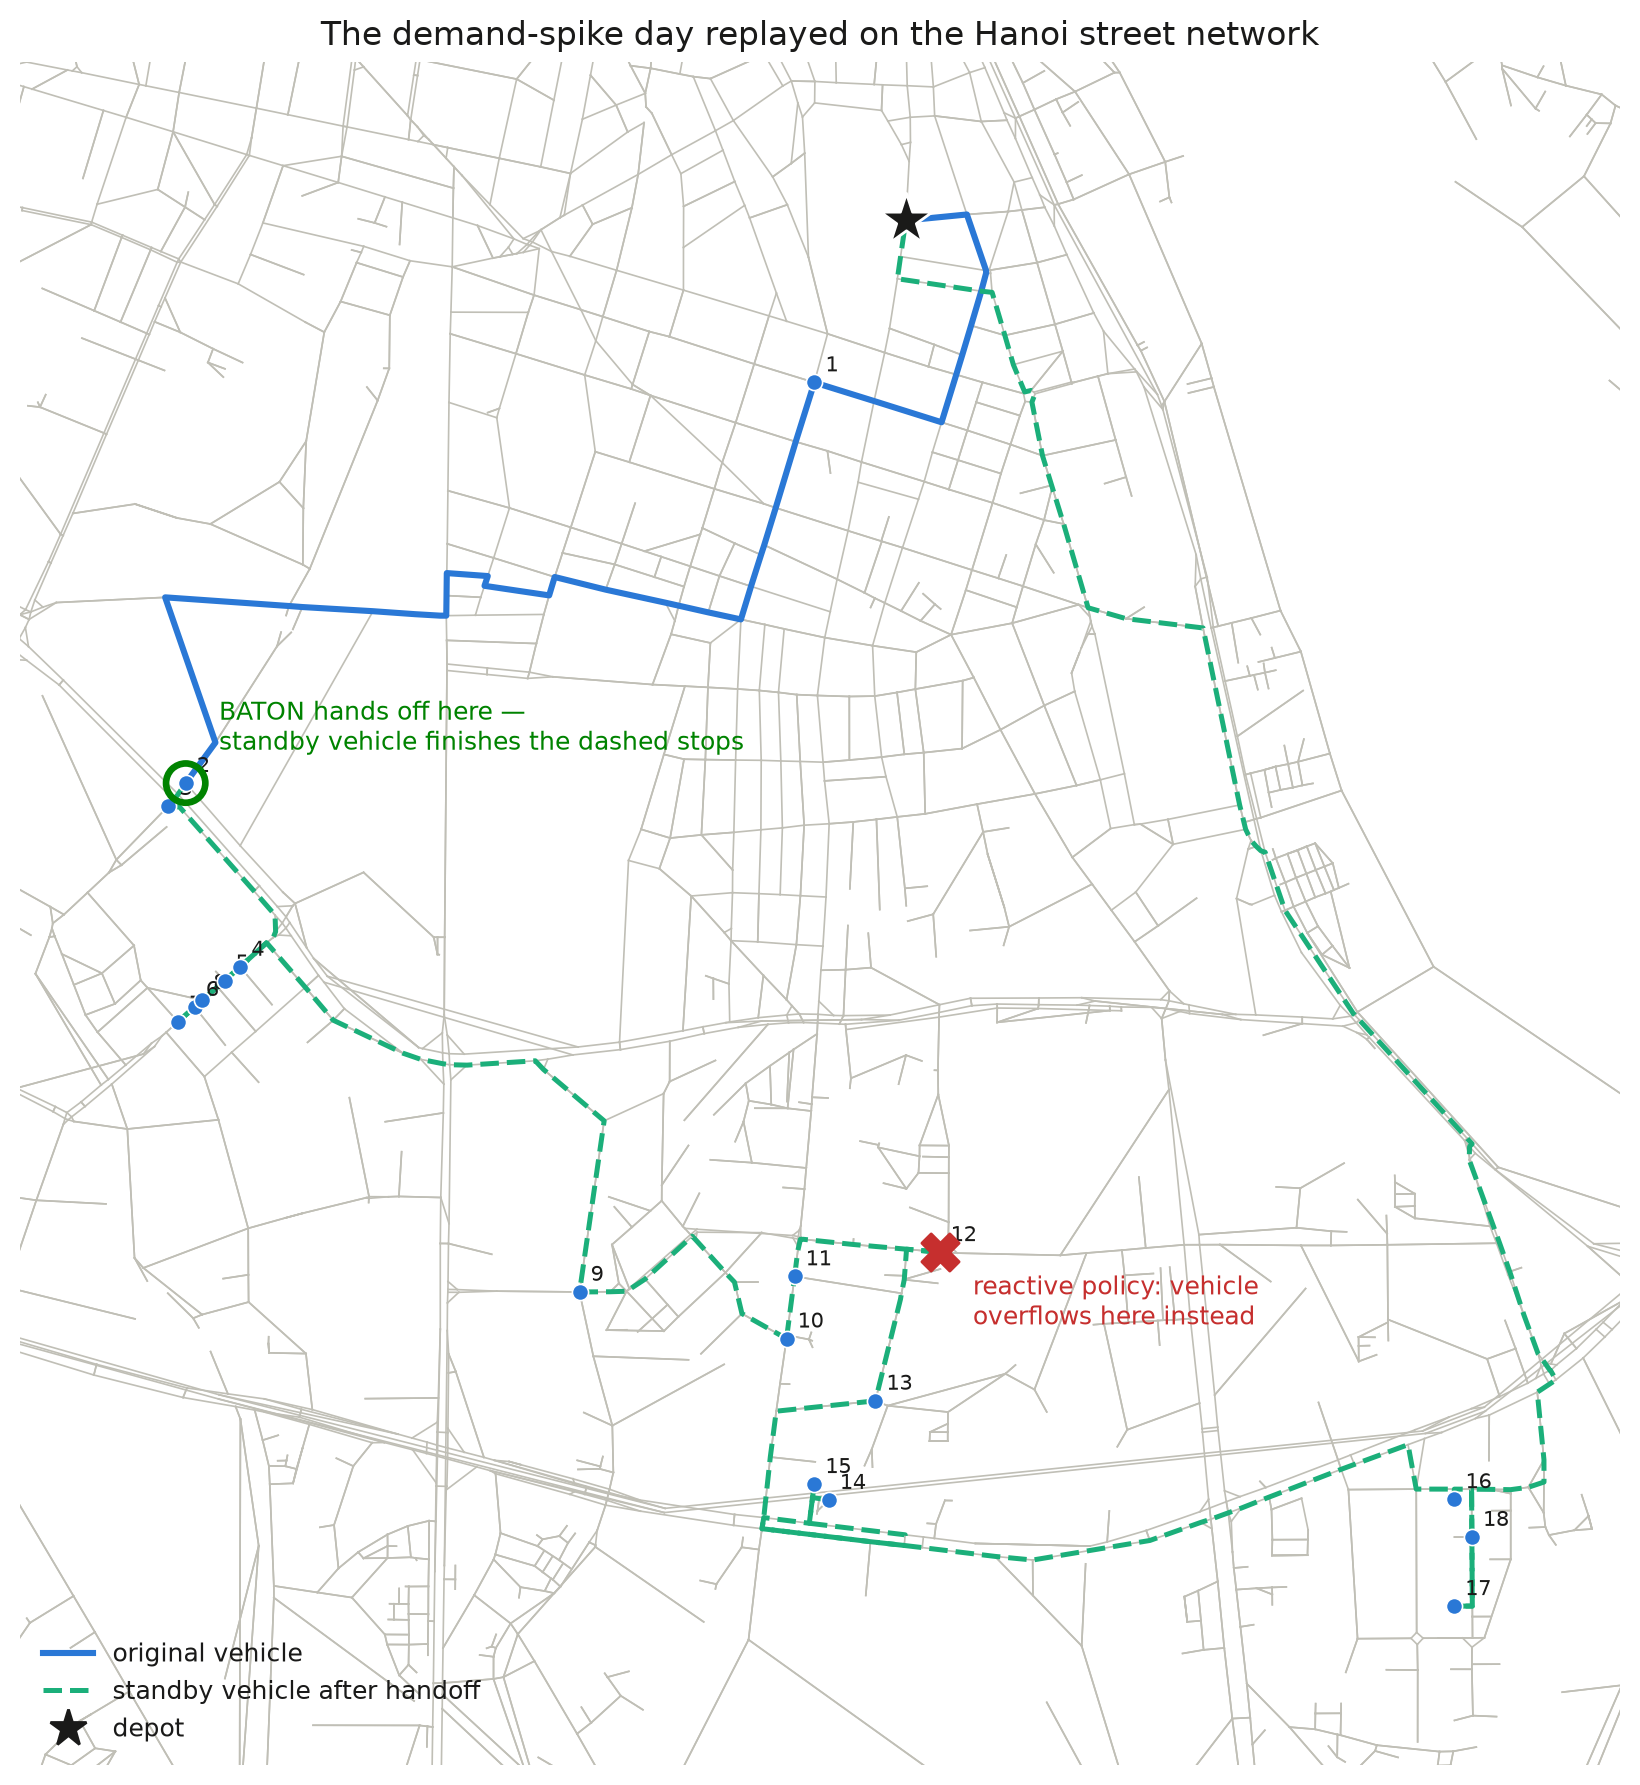
\includegraphics[width=0.92\textwidth]{figures/fig3_map_replay}
\caption{The demand-spike day of Figure~\ref{fig:explainer} replayed on
the Hanoi street network (instance \textsc{Hanoi}-100-1; grey lines are
the OSM drive network, the star is the depot, and every trail follows
real shortest road paths). The planned vehicle drives the solid route;
at the circled stop \textsc{Baton}'s estimated cost of continuing
exceeds the handoff price and a standby vehicle takes over the dashed
remainder. Under the reactive policy the same vehicle continues and
overflows at the red cross, triggering the surge-priced emergency
transfer with the rest of the route still unserved.}
\label{fig:replay}
\end{figure}

\begin{figure}[tp]
\centering
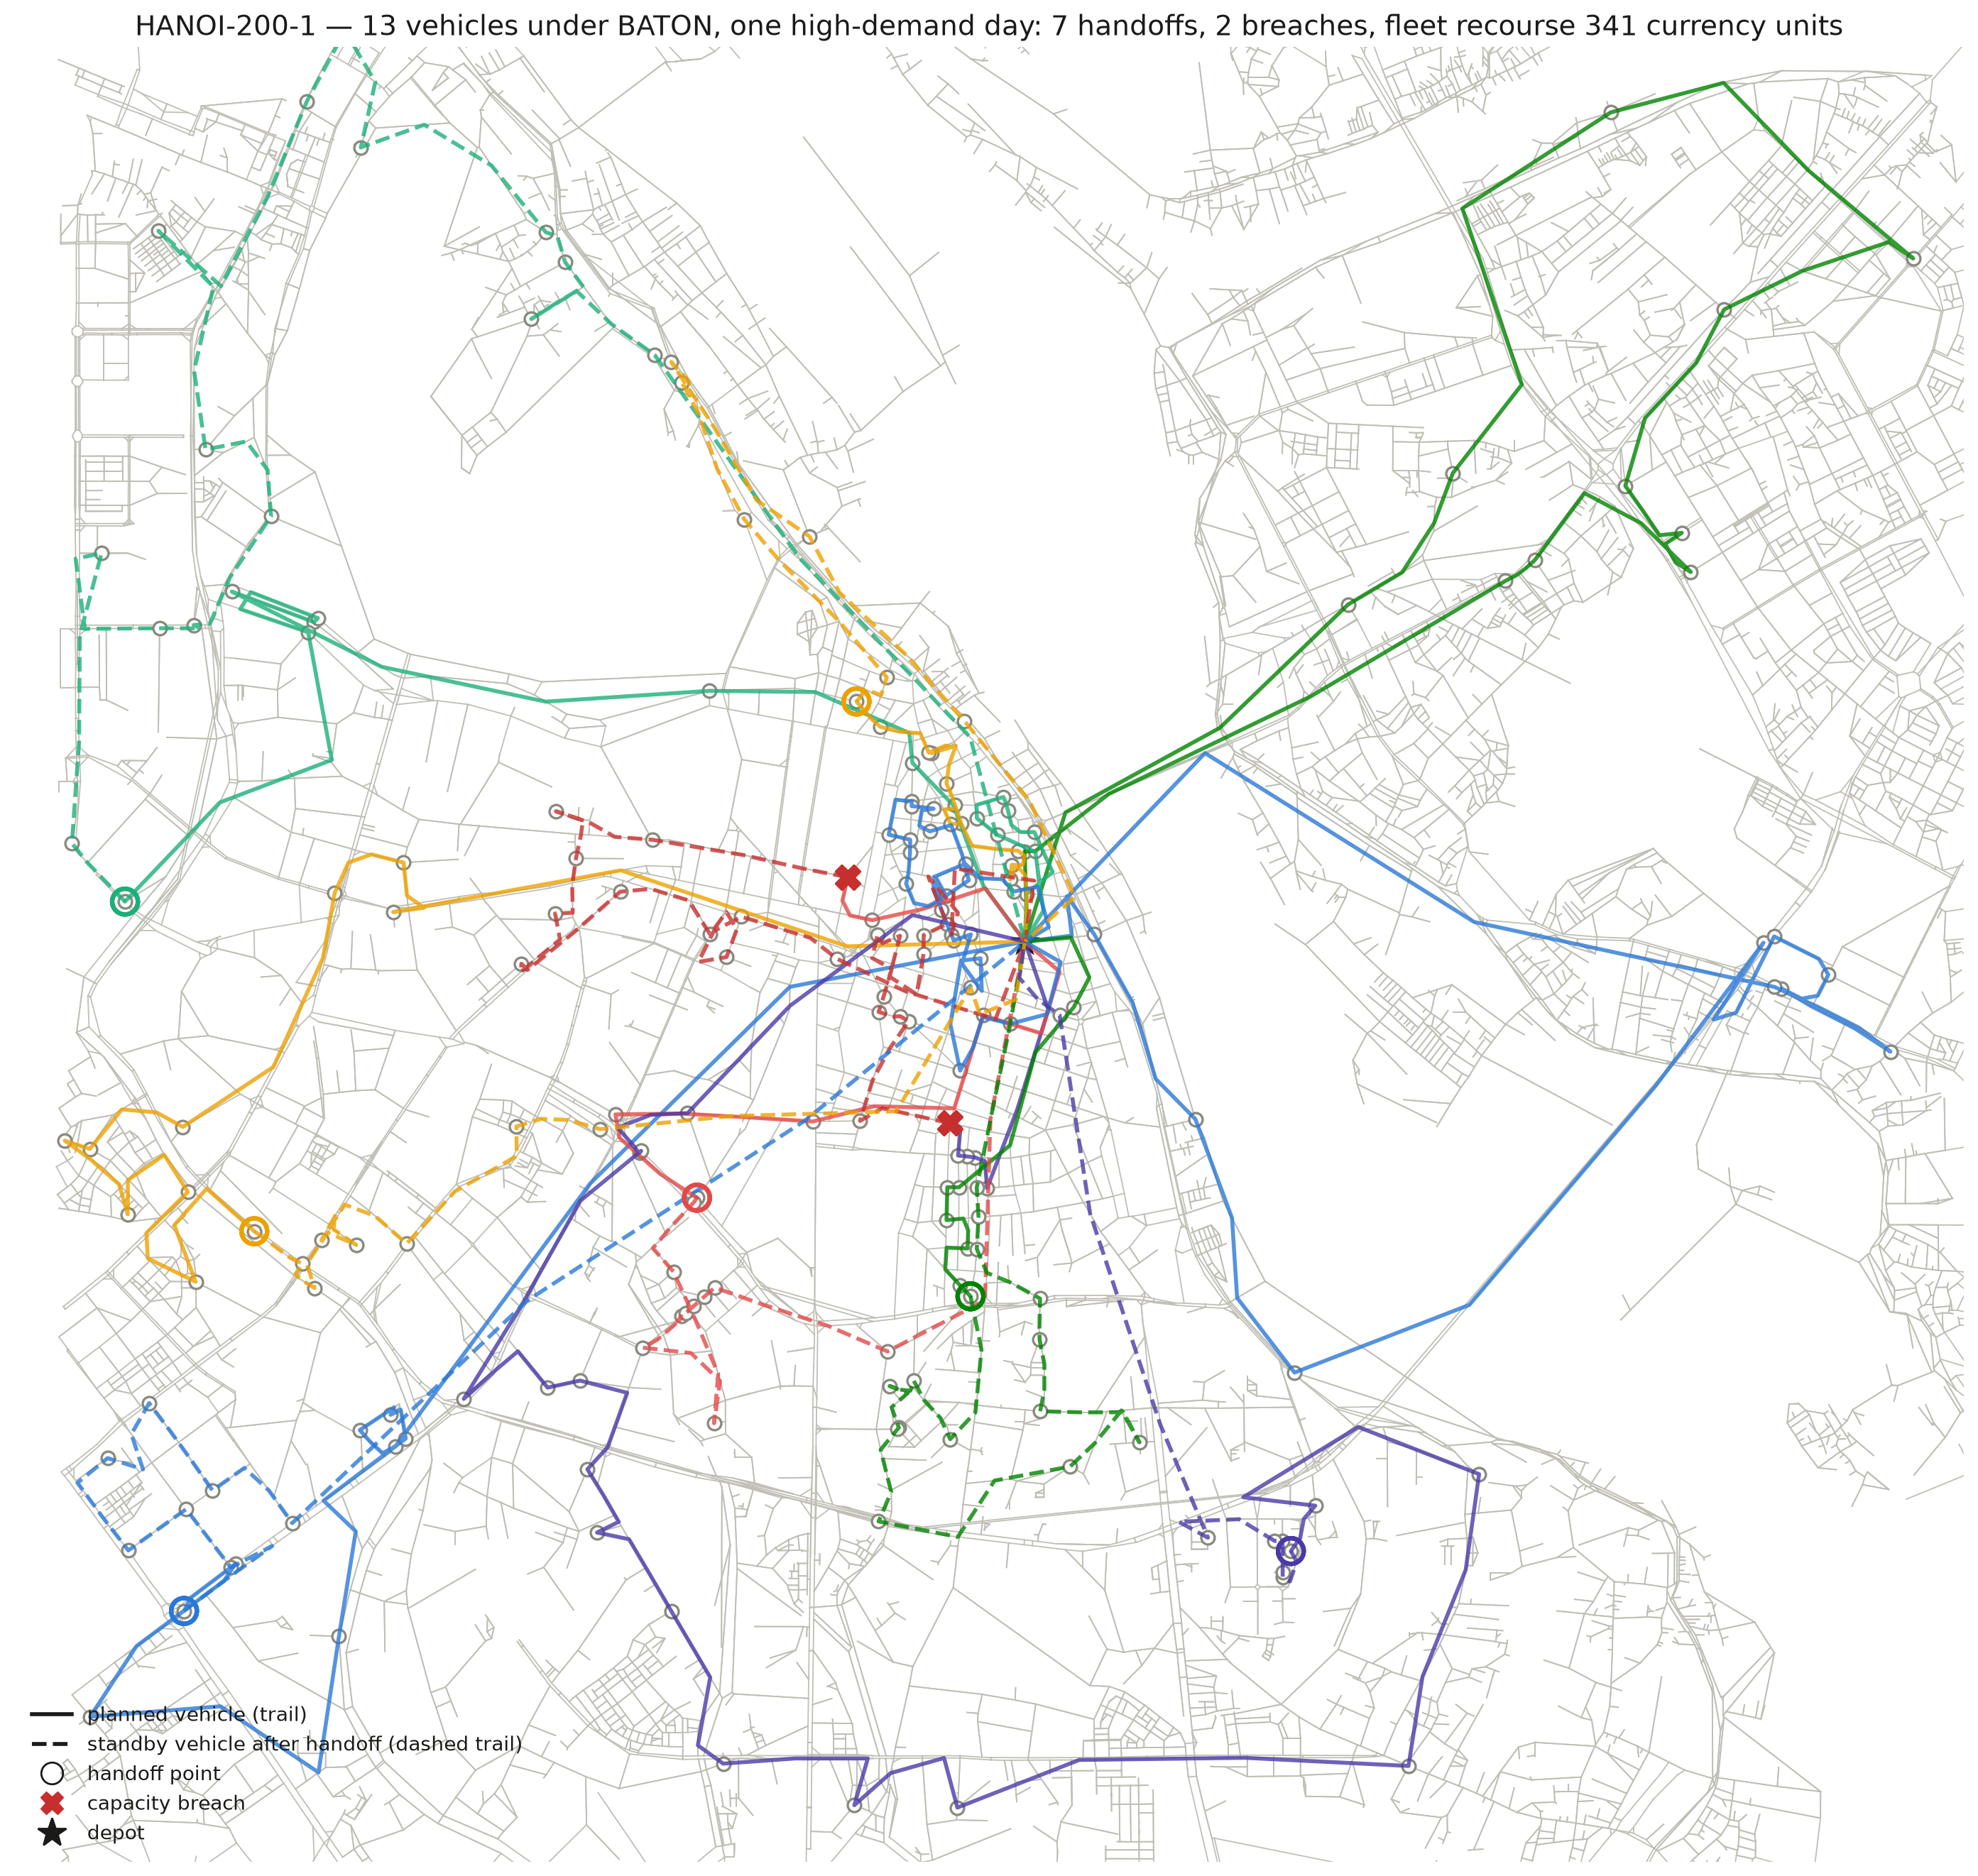
\includegraphics[width=0.92\textwidth]{figures/fig6_fleet}
\caption{One high-demand day for a full 200-customer plan on the Hanoi
network (instance \textsc{Hanoi}-200-1): thirteen vehicles execute
simultaneously under \textsc{Baton}, sharing one demand scenario. Solid
trails are planned vehicles, dashed trails the standby vehicles that
take over at the circled handoff points, and red crosses the two spikes
that outran any profitable anticipative action and fell through to the
emergency guard. Seven of thirteen routes exercised the handoff lever;
the whole day's recourse bill is \$341.}
\label{fig:fleet}
\end{figure}

The routing plans beneath every number above were certified against
mixed-integer programming bounds, using the two-commodity flow
formulation of \citet{montane2006tabu} solved by Gurobi with a
300-second budget per instance. The dual bounds certify the ALNS plans
within \certGap{} of optimality on average (worst case
\certGapMax{}), and at equal time budgets the solver's own incumbents
beat the heuristic plans on only \certBeatN{} instances---so the
execution-stage comparisons run on plans that are close to optimal and
representative of what strong planning practice produces. On 12--24-customer sub-instances, where the MIP proves
optimality outright, even the fast construction heuristic used for the
largest instances lands within 1.2--3.6\% of the optimum.

\subsection{Against learning methods, the price of over-triggering, and
two deliberate negative results}\label{sec:learning}

Because \textsc{Baton} is itself a learned policy, the natural
challenge is a more flexible learner. We re-implemented the
reinforcement-learning approach of \citet{iklassov2024rl}---a policy
network (two hidden layers of 64 units) over the observable state
(position, load, slack, price ratios, remaining-demand moments), trained
by REINFORCE with a moving-average baseline, Adam with learning rate
$3\times10^{-4}$ and batches of 256 days---over the identical routes and
training scenarios available to \textsc{Baton}, evaluating both on
identical held-out days. Table~\ref{tab:rl} reports the outcome for the
specification's 40 epochs and for 150 epochs under three seeds. The
learned policy is respectable, clearly beating the rule-based family,
but its best run saves \rlBest{} against \textsc{Baton-ho}'s
\rlBatonHo{} on the same days, losing on \rlWinN{} routes (\rlWinP{}).
The seeds cluster closely and almost quadrupling the epochs barely
moves the result, so the gap is not under-training; it is sample
efficiency. A policy-gradient method must discover the value structure
that the backward induction computes directly, and at a thousand paths
per route the regression wins, at a small fraction of the compute
(\S\ref{sec:budget}).

\begin{table}[t]
\caption{Reinforcement-learning baseline (re-implementation of the policy
architecture of Iklassov et al., 2024) versus \textsc{Baton} on the
identical 49 routes and out-of-sample test days; saving \% vs.\ the
reactive policy, \emph{higher is better}. The learned policy acts on the
handoff lever only, so \textsc{Baton-ho} is the like-for-like
comparison; the full \textsc{Baton} row adds the depot return.}
\label{tab:rl}
\centering
\begin{tabular}{l c}
\toprule
Policy & saving vs.\ reactive (\%) \\
\midrule
RL, 40 epochs & 27.2 \\
RL, 150 epochs, seed 0 & 27.4 \\
RL, 150 epochs, seed 1 & 27.3 \\
RL, 150 epochs, seed 2 & 27.3 \\
\midrule
\textsc{Baton-ho} (handoff only) & \textbf{32.9} \\
\textsc{Baton} (handoff and depot return) & \textbf{33.7} \\
\bottomrule
\end{tabular}
\end{table}


We have compared one learning architecture, and other architectures
could narrow the gap. Value-based methods such as deep Q-learning
estimate the same continuation value as \textsc{Baton} but with a
generic function class; given the monotone structure of
Proposition~\ref{prop:monotone} and a scalar state, we would expect them
to approach, not exceed, the isotonic regression at equal data.
Actor-critic methods such as PPO reduce the variance of the policy
gradient and would likely close part of the gap to \textsc{Baton-ho}
by learning a critic that plays the role of $\widehat C_k$. Attention-
and graph-based architectures pay off when the state is a large
combinatorial object---which customers remain, where the standby
vehicles are---and would become relevant for partial handoffs or
fleet-level coordination, where the state is no longer a scalar. In the
problem studied here the learner has little to discover that the
backward induction does not compute exactly, and we therefore read the
comparison as a statement about this regime rather than about
reinforcement learning in general.

\paragraph{The price of over-triggering} Proposition~\ref{prop:regret}
bounds what the myopic rule loses to the optimal one; Table~\ref{tab:regret}
evaluates both sides on the Dethloff \textsc{Det} and \textsc{SAA} plans
and the city plans, with both rules estimated on fifty thousand paths
so that the comparison reflects the functional form rather than
estimation noise. The pathwise ordering $\sigma^0 \le \sigma^\star$
holds on \regretContained{} of the test days, and the bound holds on
\regretBoundHolds{} routes. Averaged over all routes the myopic rule's
regret is \regretAll{} of the reactive cost against a bound of
\regretBoundAll{}, and the clean-day term---the cost of handing off on
days that would have ended without a breach---accounts for
\regretCleanShare{} of the bound, so unnecessary interventions are
indeed what the myopic rule pays for. The breakdown answers the
practical question of when a threshold is good enough. The regret is
smallest on tightly packed deterministic plans (\regretDet{} of reactive
cost) and on short routes of at most 12 stops (\regretShort{}), and
larger on the conservative \textsc{SAA} plans (\regretSaa{}) and on
longer routes (\regretMid{} and \regretLong{} for 13--18 and 19 or more
stops). The same pattern holds for the tuned threshold fitted on a
thousand days: its excess cost over \textsc{Baton-ho} is \thrGapDet{}
of reactive cost on \textsc{Det} plans, \thrGapCity{} on the city plans
and \thrGapSaa{} on \textsc{SAA} plans. On tight plans and on the city
routes a tuned threshold is thus a defensible simplification of the
handoff decision; on plans that carry slack, the functional form costs
money---and the larger loss there comes from the missing depot return,
which no handoff threshold can price.

\begin{table}[t]
\caption{The price of over-triggering (Proposition~\ref{prop:regret}),
per route, on 2{,}000 test days. The myopic rule and the optimal rule
are both estimated on $5\times10^4$ paths (the myopic cost-to-go by the
rollout regression, the optimal one by backward induction), so that the
comparison reflects the functional form rather than estimation noise.
Regret: excess expected cost of the myopic rule; bound: right-hand side
of~\eqref{eq:regret}; clean-day term: $\mathbb E[H_{\sigma^0}
\mathbf 1\{\sigma^0 < \sigma^\star, T = \infty\}]$; all in \% of the
reactive cost. $P(\sigma^0 < \sigma^\star)$: share of days on which the
myopic rule hands off before the optimal one; containment: share of days
with $\sigma^0 \le \sigma^\star$. Last column: excess cost of the tuned
threshold over \textsc{Baton-ho}, both fitted on $10^3$ days (\% of
reactive cost).}
\label{tab:regret}
\centering
\scriptsize
\setlength{\tabcolsep}{2.4pt}
\begin{adjustbox}{max width=\textwidth}
\begin{tabular}{l cc ccc ccc c}
\toprule
& & & & & clean-day & & $\sigma^0 < \sigma^\star$, & & thr.\ $-$ \\
Routes & $n$ & $\bar m$ & regret & bound & term & $P(\sigma^0 < \sigma^\star)$ & $T = \infty$ & contain. & \textsc{Baton-ho} \\
\midrule
Dethloff, \textsc{Det} & 256 & 7.8 & 3.8 & 7.7 & 6.9 & 16.3 & 4.7 & 100.0 & 1.0 \\
Dethloff, \textsc{SAA} & 320 & 5.9 & 6.8 & 10.9 & 8.4 & 1.6 & 0.4 & 100.0 & 3.0 \\
City, \textsc{Det} & 159 & 17.0 & 2.0 & 4.8 & 5.7 & 1.7 & 0.8 & 100.0 & 0.4 \\
\quad all, $m \le 12$ & 536 & 5.8 & 2.7 & 5.9 & 5.7 & 5.6 & 1.6 & 100.0 & 0.8 \\
\quad all, $13 \le m \le 18$ & 132 & 15.6 & 6.8 & 12.3 & 9.9 & 12.2 & 3.5 & 100.0 & 1.7 \\
\quad all, $m \ge 19$ & 67 & 20.5 & 4.5 & 9.2 & 8.9 & 4.9 & 2.0 & 100.0 & 0.9 \\
\bottomrule
\end{tabular}
\end{adjustbox}
\end{table}


\paragraph{Two negative results} Two further experiments were designed
to fail, and did, in ways that sharpen the method's justification.
First, we enriched the conditioning statistic beyond the scalar $W_k$
with exactly the features a representation-learning critique would
demand: the precision-weighted residual that is the posterior location
of the day's common demand factor, the last increment, and the running
maximum increment, fitted with monotonicity-constrained gradient-boosted
trees. On 25 real routes the enriched policy \emph{lost} to the scalar
isotonic policy on 23, by 3.2\% of cost on average, while fitting
orders of magnitude slower: at operational sample sizes the extra
features buy more estimation variance than signal, and
Proposition~\ref{prop:monotone}'s shape constraint is doing the
statistical heavy lifting. Second, the equal-data plug-in dynamic
program---the same backward induction with quantile bins in place of
the isotonic projection---collapses exactly where data are scarcest
relative to risk (on \textsc{WDRO} and \textsc{M-DRO} plans it saves
\svWDRODpN{} and \svMDRODpN{}, against \svWDROHo{} and \svMDROHo{}
for \textsc{Baton-ho}), because bins cannot pool information across
the load axis the way the monotone projection can. Together the two
null results locate \textsc{Baton} at a complexity sweet spot: one
scalar statistic, one shape constraint, no free parameters.

\subsection{Robustness to the modelling assumptions}\label{sec:robust}

This subsection probes three assumptions behind the model: that the
scalar load is a sufficient state, that days are exchangeable, and the
treatment of the post-return state.

\paragraph{Dependent demand and the sufficiency of the scalar load}
Table~\ref{tab:dependence} holds the Dethloff \textsc{Det} and
\textsc{SAA} plans fixed and re-fits and re-tests every policy under
five demand laws: Gaussian-copula correlations $\rho = 0, 0.3, 0.6, 0.9$
among the deliveries and among the pickups, and a route-level
multiplicative day factor on top of independent marginals. Three
findings stand out. First, dependence helps rather than hurts. Every
policy saves more as $\rho$ grows, because correlated demand creates
heavy days whose breaches can be foreseen from the running load; under
independence much of the risk is idiosyncratic and cannot be
anticipated. Second, \textsc{Baton} keeps the highest saving among the
implementable policies under every law, with one tie within noise
discussed below. On \textsc{Det} plans it attains
\depRhoZeroDetRatio, \depRhoSixDetRatio{} and \depRhoNineDetRatio{} of
the near-exact three-action saving at $\rho = 0$, $0.6$ and $0.9$. Third,
the monotone shape survives strong dependence. On fifty thousand paths
per route, the unconstrained binned estimate of the conditional
expected future cost given $W_k$ decreases significantly between
adjacent bins in \shapeViolZero{} of pairs under independence, where
Proposition~\ref{prop:monotone} guarantees monotonicity, and in
\shapeViolSix{} and \shapeViolNine{} of pairs at $\rho = 0.6$ and $0.9$.
The isotonic restriction is therefore justified empirically where the
theorem does not strictly apply.

The exception is instructive. Under independence the \textsc{SAA}
plans, calibrated for correlated demand, are so conservative that the
reactive policy costs only \depRhoZeroSaaReact{} per plan-day and
breaches are rare in a thousand training days. Out of sample, the
handoff interventions of the tuned threshold and of \textsc{Baton-ho}
then cost more than they prevent (\depRhoZeroSaaThr{} and
\depRhoZeroSaaHo). The position-dependent threshold learns never to act
(\depRhoZeroSaaThrK), as does \textsc{Baton} (\depRhoZeroSaaBaton), and
\textsc{Baton-cf} is marginally positive (\depRhoZeroSaaCf). This is the
small-data regime of Remark~\ref{rem:smalln}: with a few dozen breaches
per history, backward induction propagates noise, and a policy that
declines to act is the right outcome.

\begin{sidewaystable}
\caption{Robustness to the demand dependence (40 Dethloff instances,
\textsc{Det} and \textsc{SAA} plans, saving \% vs.\ reactive; plans are
held fixed and policies are re-fitted and re-tested under each demand
law; react.: expected daily recourse cost of the reactive policy per
plan, which shows how much there is to save; best implementable policy
in bold; the last two policy columns are reference points; the tuned
global threshold and the handoff-only oracle are in the replication
files). $\rho$ is
the Gaussian-copula equicorrelation among deliveries and among pickups;
the day-factor law multiplies every demand of a day by a common
lognormal factor (s.d.\ 0.25) on top of independent marginals.
$\Delta$: \textsc{Baton} minus the strongest competitor of the row
(named; \textsc{Baton} variants excluded), mean over instances with a
95\% paired bootstrap interval that re-selects the strongest competitor
in every resample. Shape test (both gates pooled): viol.\ is
the share of adjacent-bin pairs in which the unconstrained binned
estimate of $\mathbb E[\text{future cost} \mid W_k]$, fitted on
$5\times10^4$ paths per route with 25 bins, \emph{decreases}
significantly (one-sided, 2.5\% level; the rate under independence,
where monotonicity is a theorem, calibrates the test); power: share of
tests that detect a dip of 10\% or 25\% of the mean continuation cost
injected into the middle bin.}
\label{tab:dependence}
\centering
\footnotesize
\setlength{\tabcolsep}{3pt}
\begin{adjustbox}{max width=\linewidth}
\begin{tabular}{l l c ccccccc l ccc}
\toprule
& & & \multicolumn{7}{c}{saving \%} & & \multicolumn{3}{c}{shape test (\%)} \\ \cmidrule(lr){4-10}\cmidrule(lr){12-14}
Demand law & gate & react. & thr.-$k$ & two-lever & \textsc{Baton-ho} & \textsc{Baton} & \textsc{Baton-cf} & DP$^3_{50\mathrm{k}}$ & oracle$^3$ & $\Delta$ [95\% CI] & viol. & pow.$_{10}$ & pow.$_{25}$ \\
\midrule
$\rho = 0$ & \textsc{Det} & 176.4 & 10.5 & 13.1 & 10.6 & \textbf{15.5} & 15.4 & 15.5 & 48.6 & +2.0 [+1.5, +2.1] (DP$^3_N$) & 0.2 & 51 & 82 \\
 & \textsc{SAA} & 2.8 & -11.9 & -8.3 & -8.0 & -0.1 & \textbf{0.2} & 7.4 & 65.3 & -0.1 [-4.6, +2.2] (DP$_N$) & & & \\
$\rho = 0.3$ & \textsc{Det} & 180.2 & 19.1 & 20.2 & 19.3 & 21.9 & \textbf{22.5} & 22.7 & 47.6 & +1.2 [+0.9, +1.6] (DP$^3_N$) & 0.1 & 58 & 89 \\
 & \textsc{SAA} & 8.0 & 6.5 & 29.0 & 7.9 & 36.3 & \textbf{36.6} & 40.9 & 77.5 & +6.5 [+4.7, +8.4] (restock) & & & \\
$\rho = 0.6$ (bench.) & \textsc{Det} & 179.2 & 26.0 & 26.5 & 26.1 & 27.9 & \textbf{29.2} & 29.5 & 47.2 & +0.0 [-0.4, +0.4] (DP$^3_N$) & 0.1 & 72 & 97 \\
 & \textsc{SAA} & 16.5 & 19.8 & 43.9 & 20.1 & 53.7 & \textbf{53.8} & 56.4 & 78.4 & +9.7 [+8.2, +11.1] (two-lever) & & & \\
$\rho = 0.9$ & \textsc{Det} & 177.5 & 34.0 & 33.8 & 34.1 & 35.4 & \textbf{37.6} & 38.0 & 47.0 & -1.1 [-1.6, -0.7] (DP$^3_N$) & 0.0 & 88 & 97 \\
 & \textsc{SAA} & 25.9 & 32.9 & 54.4 & 33.0 & 64.5 & \textbf{65.9} & 67.7 & 78.5 & +10.2 [+8.8, +11.6] (two-lever) & & & \\
day factor, $\rho = 0$ & \textsc{Det} & 172.2 & 9.7 & 11.8 & 9.8 & \textbf{14.2} & \textbf{14.2} & 14.2 & 48.1 & +2.3 [+1.4, +3.1] (two-lever) & 0.6 & 47 & 78 \\
 & \textsc{SAA} & 5.2 & -12.7 & -2.2 & -6.9 & 7.4 & \textbf{8.0} & 12.4 & 70.2 & +1.6 [-1.6, +4.9] (restock) & & & \\
\bottomrule
\end{tabular}
\end{adjustbox}
\end{sidewaystable}


\paragraph{Non-exchangeable days} The model treats days as
exchangeable, whereas real demand has seasons, weekdays and promotions.
Table~\ref{tab:daytype} makes one day in five a promotion day, with mean
deliveries 15\% and mean pickups 35\% above normal---returns surge after
promotions---and compares three ways of fitting the policy. A pooled fit
ignores the day type; day-type-specific fits use separate histories, as
an operator can when promotions are scheduled; a stale fit is trained on
normal days only and applied unchanged on promotion days. On promotion
days \textsc{Baton} saves \dtPromoAware{} with a day-type-specific fit,
\dtPromoPooled{} with the pooled fit and \dtPromoStale{} with the stale
fit; on normal days the three coincide. The policy thus degrades
gracefully under a shift it was not trained for, because its trigger
compares costs at the current load rather than a memorised level, and a
separate fit per known day type recovers the remainder at a cost of
milliseconds. The tuned threshold gains little from any strategy,
because its single level cannot track the shift either way.

\begin{table}[t]
\caption{Non-exchangeable days (40 Dethloff instances, \textsc{Det} and
\textsc{SAA} plans; saving \% vs.\ reactive on the same days, pooled
over plans as a ratio of sums, with the ``all'' column weighting normal
and promotion days 0.8/0.2). One day
in five is a promotion day with mean deliveries $\times 1.15$ and mean
pickups $\times 1.35$. Pooled: one fit on a history that mixes both day
types; day-type-specific: separate fits, the day type being known in
advance (promotions are scheduled), each fitted on the days of its type
in the same pooled history (about 800 normal and 200 promotion days), so
that the comparison isolates the day-type information from the sample
size; stale: fitted on the normal days of that history only and applied
unchanged on promotion days. The difference between day-type-specific
and pooled \textsc{Baton} over all days is reported in the text with a
paired bootstrap interval over the 80 plans.}
\label{tab:daytype}
\centering
\footnotesize
\setlength{\tabcolsep}{3.5pt}
\begin{adjustbox}{max width=\linewidth}
\begin{tabular}{l ccc ccc}
\toprule
& \multicolumn{3}{c}{tuned threshold} & \multicolumn{3}{c}{\textsc{Baton}} \\ \cmidrule(lr){2-4}\cmidrule(lr){5-7}
Fitting strategy & normal & promotion & all & normal & promotion & all \\
\midrule
pooled fit (day type ignored) & 21.2 & 22.7 & 21.7 & 26.8 & 29.4 & 27.6 \\
day-type-specific fits & 21.2 & 22.4 & 21.6 & 26.6 & 29.7 & 27.6 \\
stale fit (normal days only) & 21.2 & 22.2 & 21.5 & 26.6 & 28.3 & 27.1 \\
\bottomrule
\end{tabular}
\end{adjustbox}
\end{table}


\paragraph{The fresh-start value and the post-return state}
Table~\ref{tab:fresh} examines the depot-return machinery of
\S\ref{sec:actions} on the three settings where it matters most or
least: Salhi--Nagy, where returns are used on about a fifth of the days;
Dethloff \textsc{SAA} plans; and the city routes, where they rarely
pay. To expose the three-action fit, all columns are computed
\emph{without} deployment selection. The first two columns measure the
error of \textsc{Baton}'s fresh-start value against the near-exact value
from fifty thousand independent paths. In-sample, the error is
\frSalhiBiasIn{} of the handoff price on Salhi--Nagy and
\frDethBiasIn{} on Dethloff; out of sample, for the same fitted
downstream policy, it is \frSalhiBiasOut{} and \frDethBiasOut{}.
Biases (i) and (ii) of \S\ref{sec:actions} are therefore small and
nearly cancel, and replacing $\widehat F_k$ by its near-exact value
changes the saving by a fraction of a point (\frSalhiThree{} against
\frSalhiFstar{} on Salhi--Nagy). Bias (iii) is different. On the
delivery-dominated city routes the three-action fit without selection
saves only \frCityThree{}, below the handoff-only policy
(\frCityHo{}): the running load drifts downward there, a return is
chosen only on unusually heavy days, and an unconditional fresh-start
value under-prices it on exactly those days. The state-conditional
fresh-start value removes the effect (\frCityCf{}) and slightly improves
the other two settings as well, so \textsc{Baton-cf} performs as well as
\textsc{Baton} \emph{with} deployment selection without needing it. The
last policy column prices the exact post-return state $x_k = -D_{\le k}$
instead of the conservative reset to zero. It raises the saving to
\frSalhiExact{} on Salhi--Nagy and \frDethExact{} on Dethloff: the
conservative convention of the main tables understates what the depot
return is worth, so the three-action results we report are
conservative. (The exact reset can exceed DP$^3_{50\mathrm{k}}$, which
is computed under the conservative convention and is therefore a
reference for that convention only.)

\begin{table}[t]
\caption{The fresh-start value and the post-return state. Bias columns:
mean error of the estimated fresh-start value $\widehat F_k$ against the
near-exact $F_k$ of DP$^3_{50\mathrm{k}}$, in \% of the handoff price;
in-sample is \textsc{Baton}'s own estimate, out-of-sample re-evaluates
the same fitted downstream policy on $5\times10^4$ independent paths.
Saving columns (\% vs.\ reactive, all \emph{without} deployment
selection, so that the three-action fit is exposed): the three-action
policy as fitted, with $\widehat F_k$ replaced by its out-of-sample
value, with $F_k$ replaced by the near-exact value, with the
state-conditional fresh-start value (\textsc{Baton-cf}), and with the
exact residual-capacity reset $x_k = -D_{\le k}$.}
\label{tab:fresh}
\centering
\scriptsize
\setlength{\tabcolsep}{2.6pt}
\begin{adjustbox}{max width=\textwidth}
\begin{tabular}{l cc c ccccc c}
\toprule
& \multicolumn{2}{c}{bias of $\widehat F_k$ (\% of $H$)} & & \multicolumn{5}{c}{three-action \textsc{Baton}, saving \%} & \\ \cmidrule(lr){2-3}\cmidrule(lr){5-9}
Benchmark & in-sample & out-of-sample & \textsc{Baton-ho} & as fitted & $F$ out-of-s. & $F$ near-exact & \textsc{cf} & exact reset & DP$^3_{50\mathrm{k}}$ \\
\midrule
Salhi--Nagy (Det) & +0.50 & +0.09 & 41.3 & 52.2 & 52.2 & 51.9 & 53.1 & 57.9 & 53.5 \\
Dethloff (SAA) & +0.00 & +0.01 & 18.9 & 51.4 & 51.4 & 51.4 & 52.2 & 54.6 & 54.6 \\
City, real shops (Det) & -1.18 & -1.05 & 9.2 & 5.6 & 5.6 & 5.9 & 9.4 & 9.9 & 10.7 \\
\bottomrule
\end{tabular}
\end{adjustbox}
\end{table}


\subsection{Shared, capacitated standby capacity}\label{sec:pool}

The default model treats standby capacity as pay-per-use from a pool
large relative to one plan (\S\ref{sec:setting}); each route then
decides alone. When instead a fixed number $S$ of standby vehicles is
reserved for the day, their holding cost $F_{\mathrm{sb}}$ is paid
whether or not they are used, a handoff costs only its marginal price
$H_k - F_{\mathrm{sb}}$, and the routes of a plan compete for the pool.
We simulate this coupling exactly. On every test day the routes of a
plan run simultaneously, handoff requests are served first come, first
served in the order of the time at which they arise along the routes,
and a route whose request is refused continues under its fallback menu
(continue or return to the depot, fitted by the same backward induction
with the handoff removed). Two policies are compared. The \emph{naive}
policy decides every route at the marginal price and ignores the cap.
The \emph{shadow-priced} policy decides every route at the price
$H_k - F_{\mathrm{sb}} + \lambda$, where the shadow price $\lambda \ge 0$
of a standby vehicle is chosen, for each plan and pool size, on the
training days; it decouples the routes, which can then still be
decided one at a time. For each plan we compute the expected daily
total---holding plus recourse---for every pool size from $S = 0$ to one
vehicle per route, and report the cost-minimising size $S^\star$.

Table~\ref{tab:pool} gives two answers. The first concerns the pool
size. At the default holding cost, reserving even one standby vehicle
for a single plan never pays: the cost-minimising pool size is $S^\star =
0$ for every plan, because the expected number of handoffs per plan-day
is far below one, and a vehicle held for one plan mostly waits. (Under
pay-per-use, the pool that covers 95\% of days has a median of
\poolBatonMed{} and a maximum of \poolBatonMax{} vehicles per plan for
\textsc{Baton}, and \poolHoMed{} and \poolHoMax{} for \textsc{Baton-ho},
whose only lever is the handoff.) Standby capacity is economical only
when it is shared across many plans, so that its holding cost is spread
over the handoffs of the whole operation, which is the pay-per-use
regime of our default model. The second answer concerns the coupling.
Given a cap, deciding each route with a shadow price is clearly better
than ignoring the cap. A naive route requests handoffs it may be
refused, and a refused route has already let its load climb past the
point at which a return would have paid. With no standby vehicle at all,
shadow pricing lowers the daily recourse cost by \poolDethGainZero{} on
the Dethloff plans and \poolCityGainZero{} on the city plans; with one
vehicle for the plan, by \poolDethGainOne{} and \poolCityGainOne. The
shadow price decouples the routes, so the policy is still fitted one
route at a time, and the depot return is the lever that makes a small
or empty pool tolerable.

\begin{table}[t]
\caption{Shared, capacitated standby pool: expected daily recourse cost per
plan (currency units, excluding the holding cost of reserved vehicles).
Pay-per-use: the default model (pooled capacity, day rate billed per
handoff). Reserved pool of $S$ vehicles: each held vehicle costs
$F_{\mathrm{sb}} = 20$ per day whether or not it is used, a handoff then
costs its marginal price $H_k - F_{\mathrm{sb}}$, requests are served
first come, first served in the order of their time along the routes, and
a route whose request is refused continues under its fallback menu
(continue or return to the depot). Naive: every route decides at the
marginal price and ignores the cap. Shadow: every route decides at
$H_k - F_{\mathrm{sb}} + \lambda$, with the shadow price $\lambda$ of a
standby vehicle chosen on the training days. $S^\star$: pool size
minimising holding plus recourse for the shadow-priced policy.}
\label{tab:pool}
\centering
\footnotesize
\setlength{\tabcolsep}{3.5pt}
\begin{adjustbox}{max width=\textwidth}
\begin{tabular}{l cc c cc cc cc c}
\toprule
& & & pay-per- & \multicolumn{2}{c}{$S = 0$} & \multicolumn{2}{c}{$S = 1$} & \multicolumn{2}{c}{$S = 2$} & \\ \cmidrule(lr){5-6}\cmidrule(lr){7-8}\cmidrule(lr){9-10}
Benchmark & plans & routes & use & naive & shadow & naive & shadow & naive & shadow & $S^\star$ \\
\midrule
Dethloff (SAA plans) & 40 & 9.5 & 8.3 & 9.9 & 8.3 & 9.0 & 8.2 & 8.5 & 8.1 & 0.0 \\
City (Det plans) & 19 & 8.4 & 33.4 & 38.3 & 36.7 & 34.2 & 33.0 & 31.4 & 30.5 & 0.0 \\
\bottomrule
\end{tabular}
\end{adjustbox}
\end{table}



\subsection{Data and computing budgets}\label{sec:budget}

Every data-driven policy in the preceding tables was fitted on the same
$10^3$ training days per instance; only the two reference programs saw
more. Table~\ref{tab:budget} and Figure~\ref{fig:budget} vary the
history from $10^2$ to $2\times10^4$ days per route, on the same test
days, for \textsc{Baton}, the label-corrected tuned threshold and the
equal-data dynamic program.

\textsc{Baton} beats the tuned threshold at every history length we
tested. With only 100 days per route it saves \budDethDetSmall{} on
\textsc{Det} plans and \budDethSaaSmall{} on \textsc{SAA} plans, where
the threshold saves \budDethSaaThrSmall{} and the equal-data dynamic
program is no better. The isotonic projection pools information along
the load axis, whereas quantile bins need many paths per bin before
their estimates stabilise, which is why DP$_N$ trails even the
threshold on short histories. As the history grows, \textsc{Baton}
approaches the near-exact references. On the \textsc{SAA} plans it
reaches \budDethSaaLarge{} at $2\times10^4$ days against
\budDethSaaDpThree{} for DP$^3_{50\mathrm{k}}$, and on the city routes it
slightly exceeds the binned references (\budCityLarge{} against
\budCityDp{}), the binned programs being only near-exact themselves.
The gaps in Table~\ref{tab:grand} between \textsc{Baton} and the
references are therefore the finite-sample cost of learning from a
thousand days, not a structural shortfall of the policy. The clairvoyant
oracle's lead, by contrast, does not shrink with data: it is the value
of knowing the future.

Table~\ref{tab:timing} separates offline from online computation on one
CPU core. Offline, fitting \textsc{Baton-ho} takes \timeBatonHoMs{} per
route and the full policy, including the fresh-start valuations and
deployment selection, \timeBatonMs; the grid-tuned competitors cost
about the same or more, because tuning re-simulates the training days
for every candidate parameter. Online, every cost-comparison policy
makes one lookup in a monotone step function and two comparisons per
stop, about \timeOnlineUs{} per decision through the fitted breakpoints.
The reinforcement-learning baseline of \S\ref{sec:learning} is the
exception: on the same CPU its training takes \rlTrainMin--\rlTrainMax{}
minutes for the \nRL{} routes of Table~\ref{tab:rl}, against
\rlBatonFitS{} seconds for fitting \textsc{Baton} on the same routes, so
the comparison of Table~\ref{tab:rl} is, if anything, generous to the
learner in computing budget and identical in data.

\begin{figure}[t]
\centering
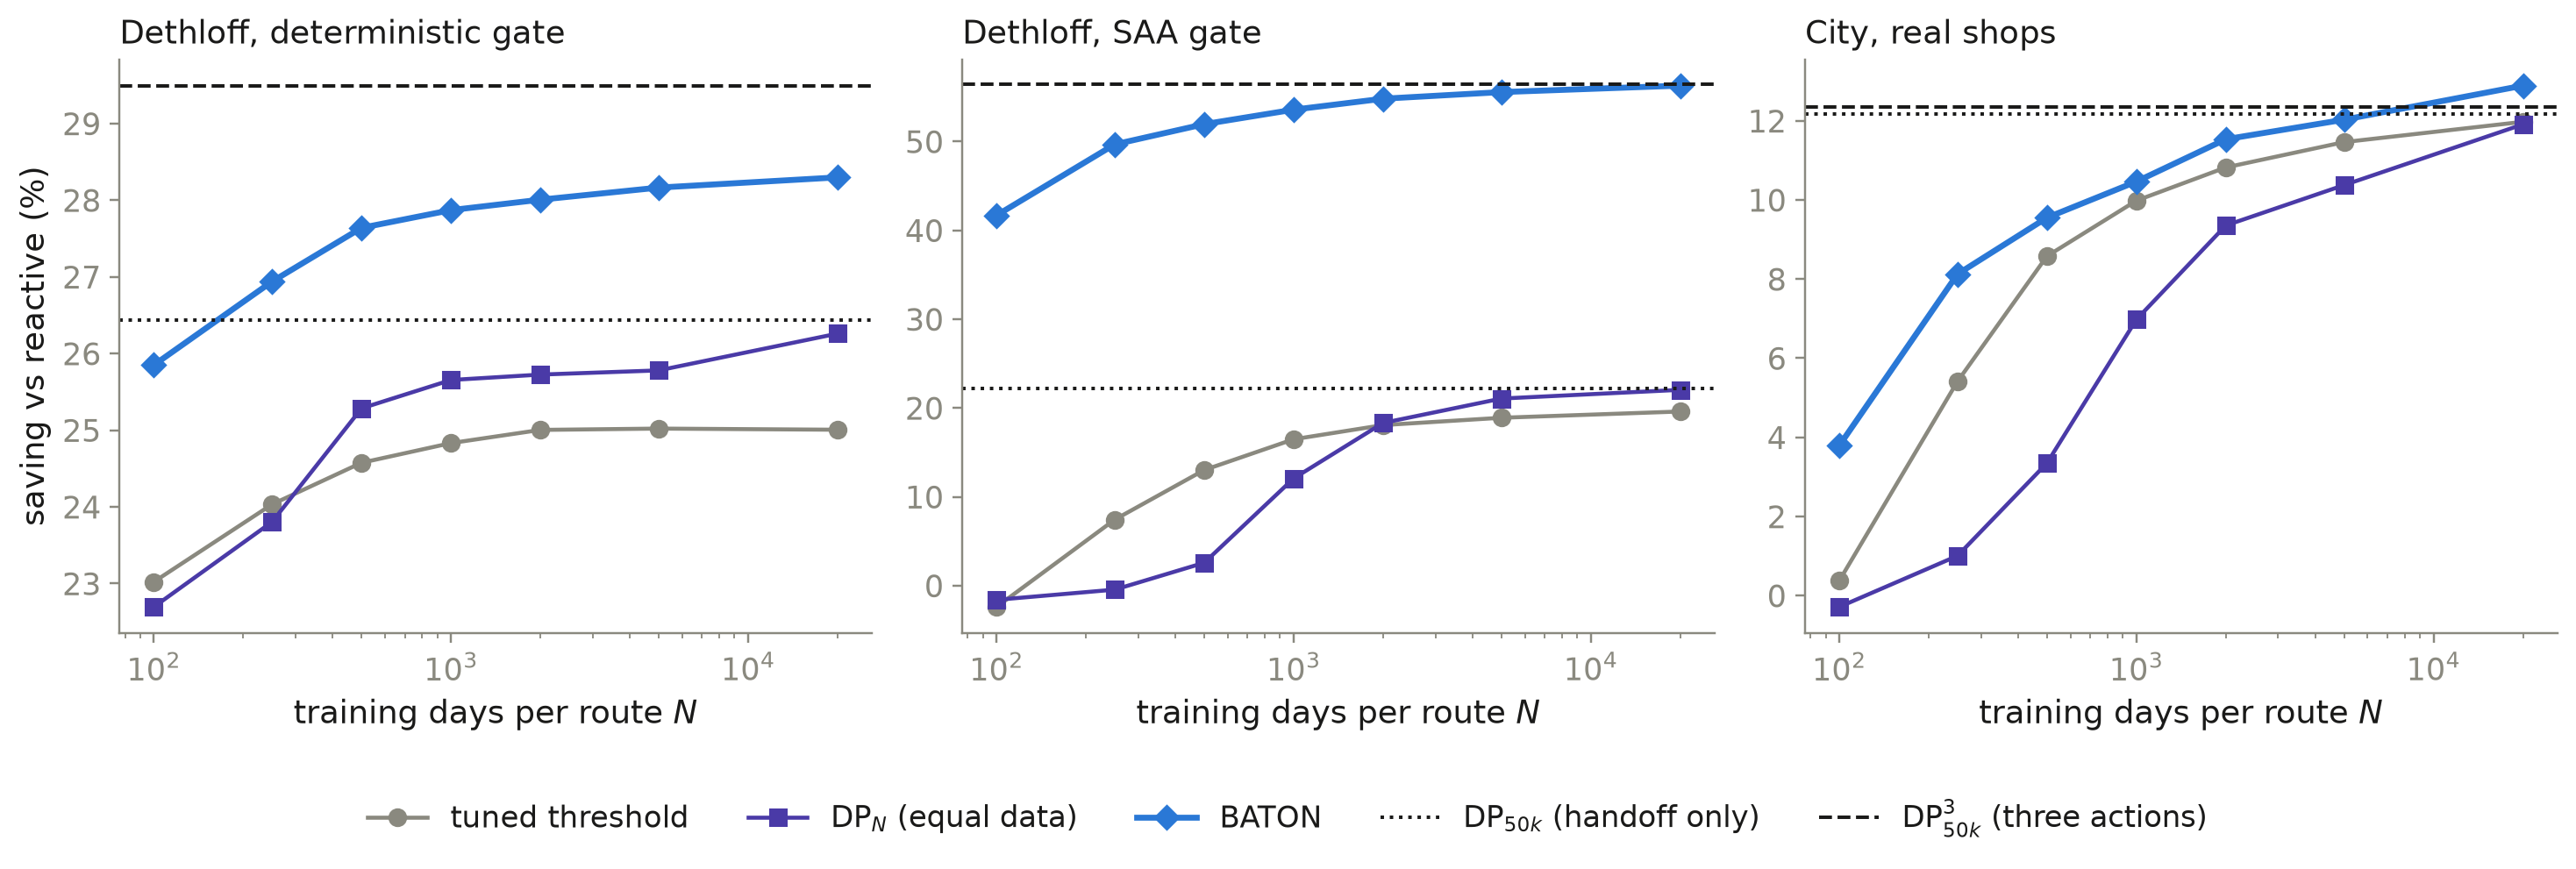
\includegraphics[width=\textwidth]{figures/fig8_budget}
\caption{Saving over the reactive policy as a function of the number of
training days per route (log scale), on identical test days. Horizontal
lines: the near-exact handoff-only and three-action dynamic programs
fitted on $5\times10^4$ days.}
\label{fig:budget}
\end{figure}

\begin{table}[t]
\caption{Training-data budget: saving \% vs.\ reactive as a function of
the number $N$ of training days per route (same test days throughout).
thr.: label-corrected tuned threshold; DP$_N$: plug-in dynamic program
at equal data; \textsc{Baton} with deployment selection. The last row
gives the near-exact references (handoff-only / three-action).}
\label{tab:budget}
\centering
\footnotesize
\setlength{\tabcolsep}{3.5pt}
\begin{adjustbox}{max width=\textwidth}
\begin{tabular}{r ccc ccc ccc}
\toprule
& \multicolumn{3}{c}{Dethloff, \textsc{Det}} & \multicolumn{3}{c}{Dethloff, \textsc{SAA}} & \multicolumn{3}{c}{City, \textsc{Det}} \\ \cmidrule(lr){2-4}\cmidrule(lr){5-7}\cmidrule(lr){8-10}
$N$ & thr. & DP$_N$ & \textsc{Baton} & thr. & DP$_N$ & \textsc{Baton} & thr. & DP$_N$ & \textsc{Baton} \\
\midrule
100 & 23.0 & 22.7 & 25.8 & -2.4 & -1.6 & 41.7 & 0.4 & -0.3 & 3.8 \\
250 & 24.0 & 23.8 & 26.9 & 7.4 & -0.5 & 49.7 & 5.4 & 1.0 & 8.1 \\
500 & 24.6 & 25.3 & 27.6 & 13.0 & 2.6 & 52.0 & 8.6 & 3.3 & 9.6 \\
1{,}000 & 24.8 & 25.7 & 27.9 & 16.5 & 12.1 & 53.6 & 10.0 & 7.0 & 10.5 \\
2{,}000 & 25.0 & 25.7 & 28.0 & 18.1 & 18.3 & 54.8 & 10.8 & 9.4 & 11.5 \\
5{,}000 & 25.0 & 25.8 & 28.2 & 18.9 & 21.1 & 55.6 & 11.5 & 10.4 & 12.0 \\
20{,}000 & 25.0 & 26.3 & 28.3 & 19.6 & 22.0 & 56.3 & 12.0 & 11.9 & 12.9 \\
\midrule
ref.: DP$_{50\mathrm{k}}$ / DP$^3_{50\mathrm{k}}$ &  & 26.4 & 29.5 &  & 22.2 & 56.4 &  & 12.2 & 12.3 \\
\bottomrule
\end{tabular}
\end{adjustbox}
\end{table}


\begin{table}[t]
\caption{Offline fitting time per route (single CPU core, milliseconds;
median and 90th percentile over 102 routes of ten Dethloff
\textsc{SAA} plans and four city plans). Every policy is fitted on the
same $10^3$ training days except the two reference programs. Tuning by
grid search on realised training cost is included; the
position-dependent threshold includes the fits of its two starting
points. The online decision
of every cost-comparison policy is one lookup in a monotone
piecewise-linear function and two comparisons: 1.2\,$\mu$s per decision through the
fitted breakpoints (63\,$\mu$s through the
scikit-learn prediction call).}
\label{tab:timing}
\centering
\footnotesize
\setlength{\tabcolsep}{3.5pt}
\begin{adjustbox}{max width=\linewidth}
\begin{tabular}{l c cc}
\toprule
Policy & training days & median & p90 \\
\midrule
tuned threshold (peak label) & $10^3$ & 63.9 & 100.4 \\
position-dependent threshold & $10^3$ & 155.7 & 343.7 \\
$\pi_3$ rule (grid-tuned) & $10^3$ & 4.9 & 7.6 \\
rollout & $10^3$ & 6.1 & 10.7 \\
cost-scaled rollout & $10^3$ & 47.9 & 81.6 \\
depot-return restocking & $10^3$ & 4.8 & 7.4 \\
two-lever rule (joint grid) & $10^3$ & 413.4 & 677.6 \\
DP$_N$ (equal data) & $10^3$ & 3.1 & 5.0 \\
DP$^3_N$ (equal data) & $10^3$ & 7.0 & 14.4 \\
\textsc{Baton-ho} & $10^3$ & 7.2 & 11.3 \\
\textsc{Baton} (incl.\ deployment selection) & $10^3$ & 24.2 & 49.2 \\
\textsc{Baton-cf} & $10^3$ & 25.0 & 58.6 \\
DP$_{50\mathrm{k}}$ (reference, $5\times10^4$ paths) & $5\times10^4$ & 110.0 & 170.7 \\
DP$^3_{50\mathrm{k}}$ (reference, $5\times10^4$ paths) & $5\times10^4$ & 279.8 & 573.8 \\
\bottomrule
\end{tabular}
\end{adjustbox}
\end{table}



\subsection{Economic and spatial sensitivity}\label{sec:sensitivity}

A recourse policy earns its keep only if its advantage survives changes
in the prices that define it. Table~\ref{tab:costsens} and
Figure~\ref{fig:costsens} sweep the four managerial cost levers one at
a time around the defaults: the standby day rate, the emergency
callout, the surge multiplier, and the per-customer lateness price.
\textsc{Baton} leads in every configuration, but the instructive
content is \emph{how}. When standby capacity is dear
($F_{\mathrm{sb}} = 35$), the threshold family collapses to
\dearSbThresh{}---its handoffs cost more than they save---while
\textsc{Baton} holds \dearSbBaton{} by shifting its mix toward depot
returns, ending far above the handoff-only clairvoyant bound
(\dearSbOrc{}). When lateness is expensive, depot returns lose their
appeal and the mix shifts back toward handoffs. The last row sets the
standby rate so high ($F_{\mathrm{sb}} = 60$) that a handoff costs more
than an emergency at late stops, violating
Inequality~\eqref{eq:prices}. Nothing in the theory depends on that
inequality (Assumption~\ref{ass:prices}), and the policy behaves
accordingly: it stops handing off where the handoff is dominated,
relies on depot returns, and saves \sbSixtyBaton{}, while the tuned
threshold saves \sbSixtyThresh{} and the handoff-only restriction
\sbSixtyHo{}. No parameter changes across these worlds; the policy
simply re-prices its levers.

\begin{table}[t]
\caption{Sensitivity of the recourse saving (\%, \emph{higher is
better}; best non-clairvoyant value per row in bold) to the fleet-economics
parameters, one factor at a time around the defaults (12 Dethloff
instances, \textsc{Det} and \textsc{SAA} gates; the baseline row is
computed on the same 12 instances). \textsc{Baton} re-balances its
action mix as prices move and leads in every configuration. In the last
row the standby rate exceeds the emergency price at late stops, so
Inequality~\eqref{eq:prices} fails there.}
\label{tab:costsens}
\centering
\footnotesize
\setlength{\tabcolsep}{4pt}
\begin{adjustbox}{max width=\textwidth}
\begin{tabular}{l ccccc}
\toprule
Configuration & restock & threshold & \textsc{Baton-ho} &
\textsc{Baton} & oracle (HO) \\
\midrule
baseline & 28.2 & 24.9 & 29.0 & \textbf{48.0} & 44.5 \\
cheap emergencies ($F_{\mathrm{emg}}{=}25$) & 23.4 & 13.0 & 18.0 & \textbf{40.1} & 31.0 \\
dear emergencies ($F_{\mathrm{emg}}{=}60$) & 32.9 & 36.0 & 39.6 & \textbf{55.2} & 55.3 \\
cheap standby ($F_{\mathrm{sb}}{=}10$) & 28.2 & 37.5 & 41.7 & \textbf{52.7} & 57.7 \\
dear standby ($F_{\mathrm{sb}}{=}35$) & 28.2 & 8.8 & 13.1 & \textbf{42.6} & 24.8 \\
low SLA price ($p_{\mathrm{late}}{=}0.5$) & 33.1 & 22.3 & 26.4 & \textbf{49.0} & 42.0 \\
high SLA price ($p_{\mathrm{late}}{=}3$) & 23.6 & 28.5 & 32.3 & \textbf{47.0} & 47.6 \\
mild surge ($s_{\mathrm{emg}}{=}1.5$) & 27.4 & 20.6 & 24.8 & \textbf{44.7} & 40.3 \\
heavy surge ($s_{\mathrm{emg}}{=}4$) & 29.9 & 30.4 & 34.1 & \textbf{52.0} & 49.5 \\
standby above emergency ($F_{\mathrm{sb}}{=}60$) & 28.2 & 1.4 & 2.1 & \textbf{36.8} & 5.0 \\
\bottomrule
\end{tabular}
\end{adjustbox}
\end{table}


\begin{figure}[t]
\centering
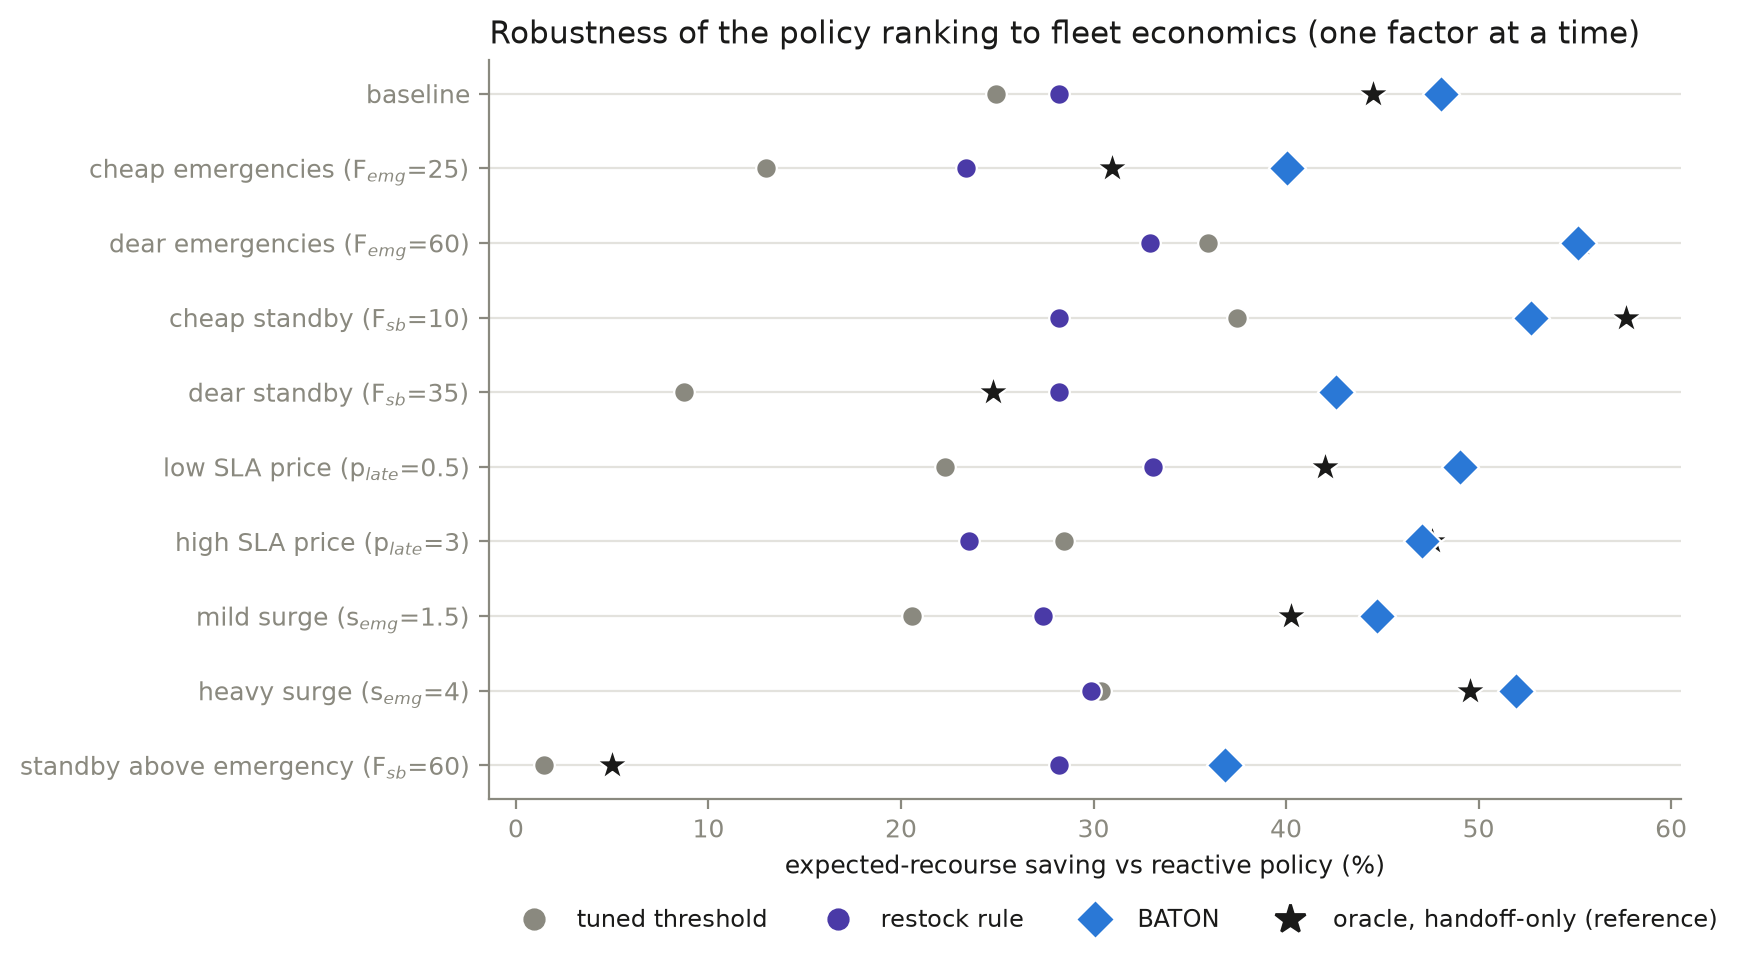
\includegraphics[width=\textwidth]{figures/fig5_costsens}
\caption{Sensitivity of the policy ranking to the fleet economics, one
factor at a time. \textsc{Baton} (diamonds) leads in every
configuration, re-balancing between handoffs and depot returns as the
relative prices move.}
\label{fig:costsens}
\end{figure}

The spatial-structure experiment closes the study. For each city
instance we generated a twin with identical demands and identical seeds
but customers scattered uniformly over the street network rather than
placed at real shops; Figure~\ref{fig:shops} shows the pair for the
200-customer Hanoi instance, and the visual difference is the
experiment: real retail concentrates around the commercial core while
the uniform convention spreads demand into residential and peripheral
blocks. The real retail clustering shortens optimal
routes by \shopTravelSaving{} on average---uniform spatial conventions
materially overstate travel in urban simultaneous pickup-and-delivery
---while the execution-policy ranking and \textsc{Baton}'s margins are
unchanged between the twins. The policy conclusions of this paper do
not depend on where customers stand; the absolute economics do, which
is precisely why we report both.

\begin{figure}[tp]
\centering
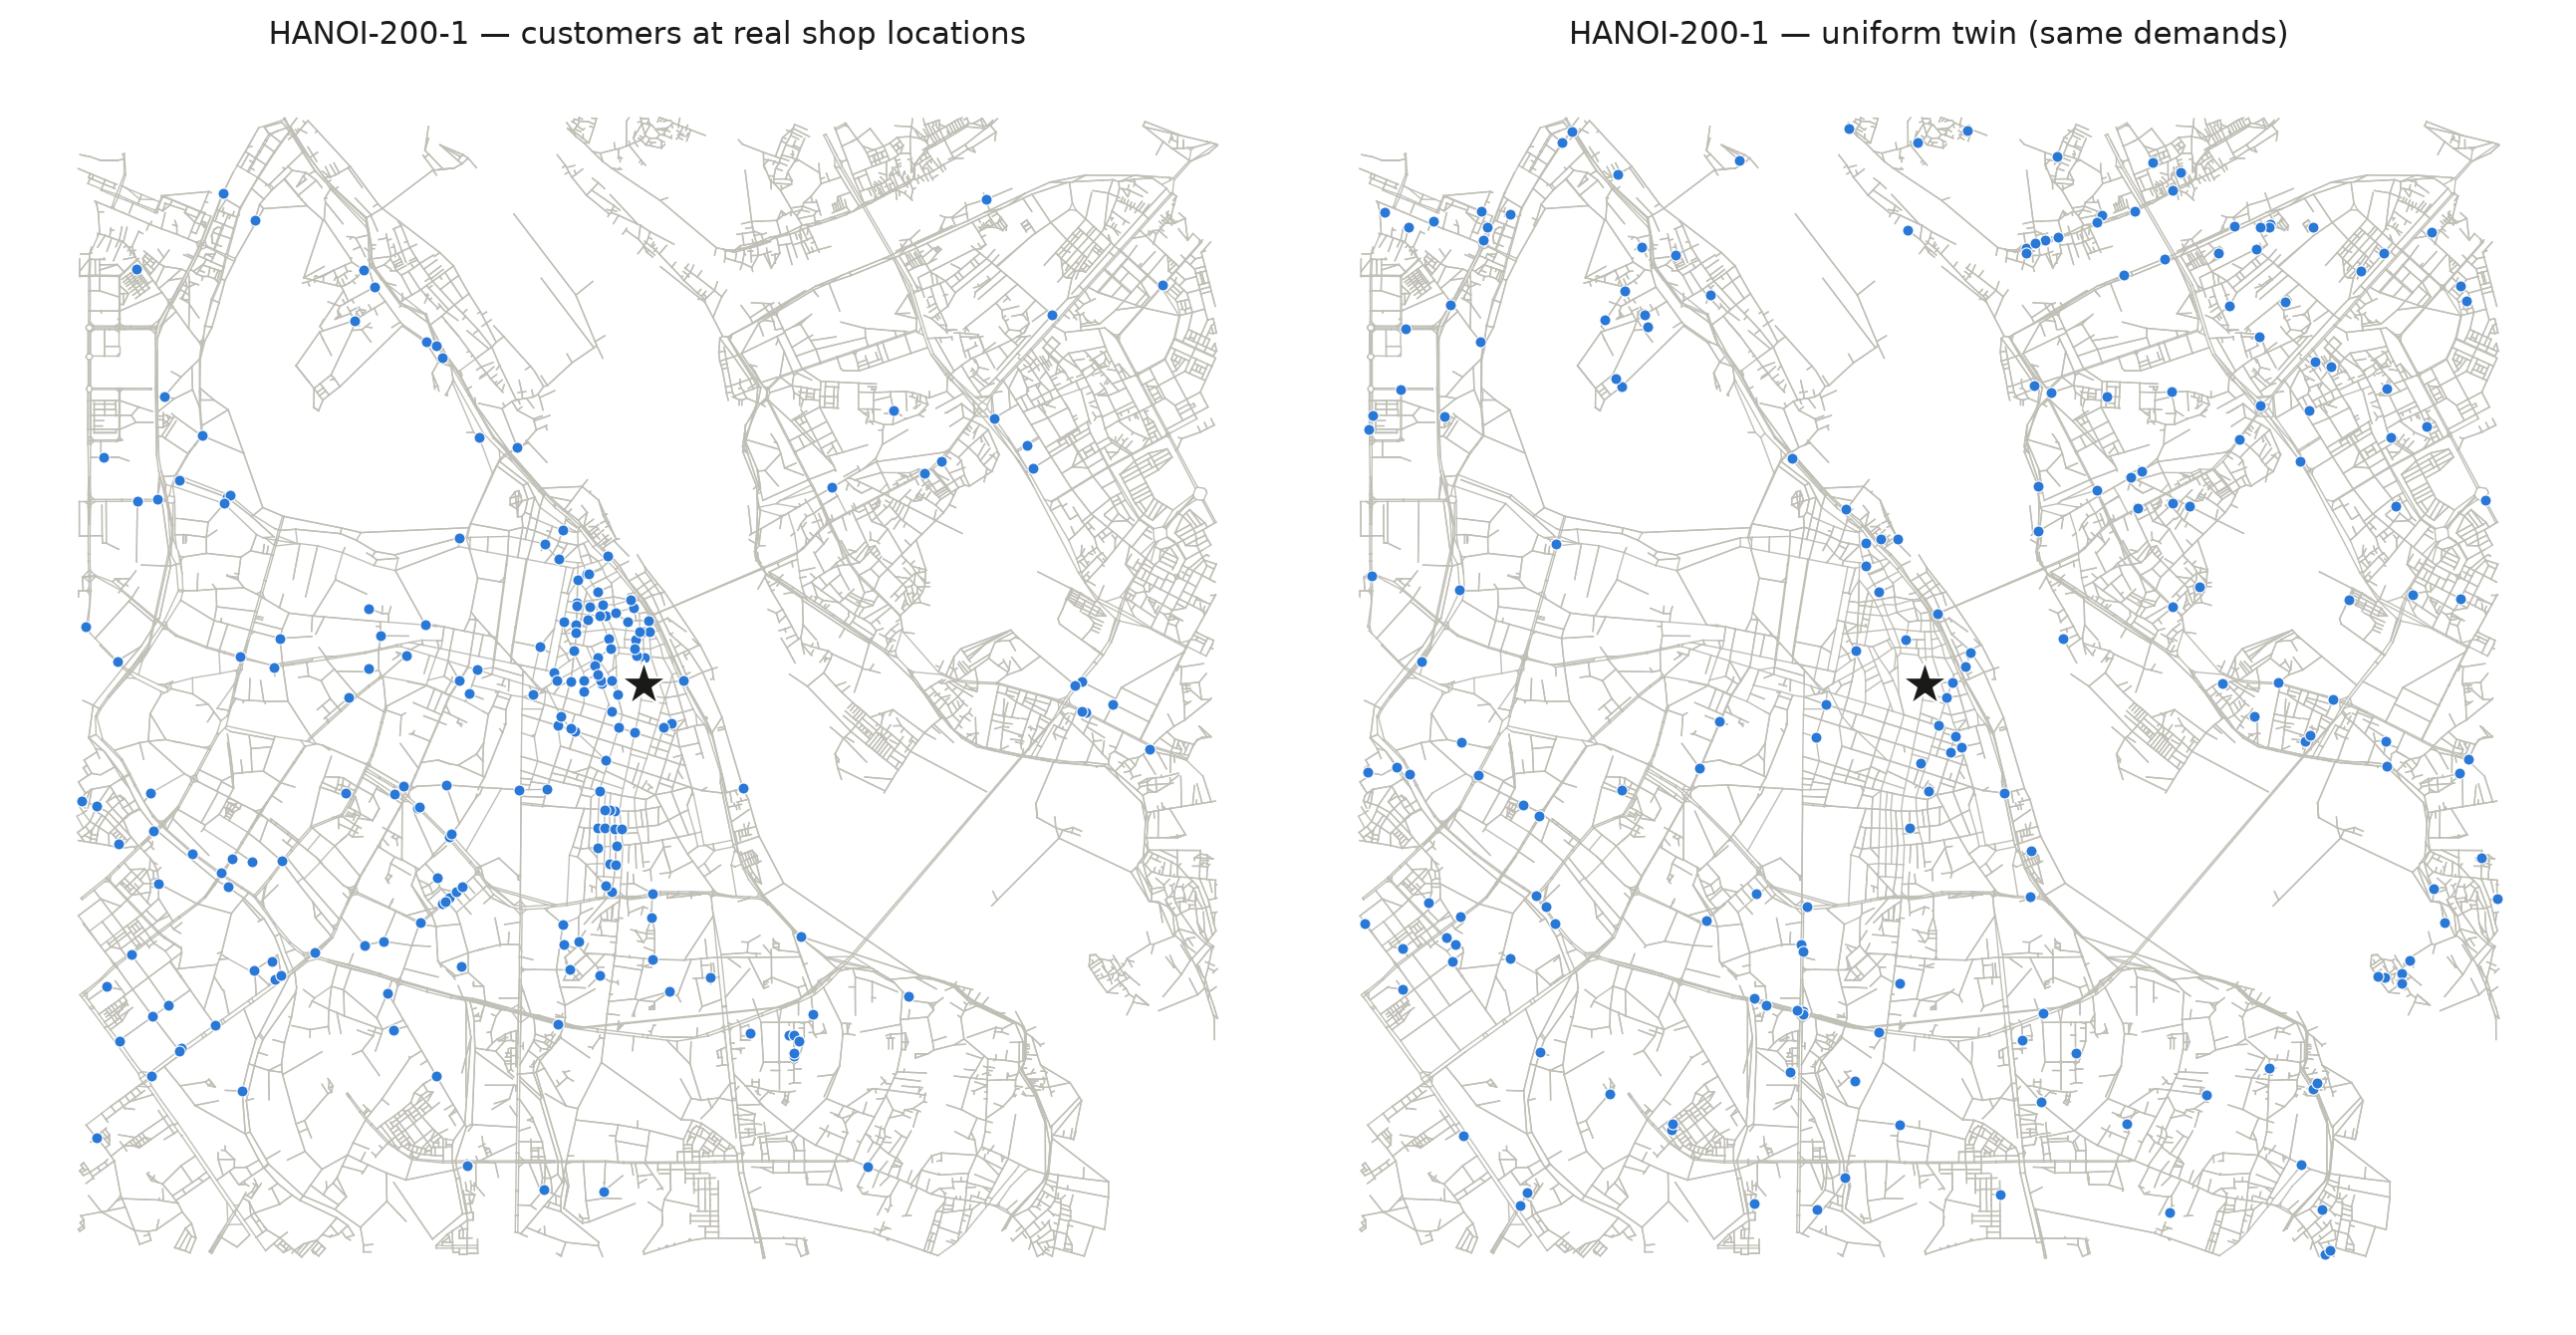
\includegraphics[width=\textwidth]{figures/fig7_shops_vs_uniform}
\caption{The spatial-structure twins for \textsc{Hanoi}-200-1 on the
OSM drive network (star: depot). Left: the 200 customers at real
OpenStreetMap shop locations, clustered along the retail corridors
around the commercial centre. Right: the uniform twin---identical
demand draws, customers scattered uniformly over the same street
network. Real clustering shortens optimal routes by
\shopTravelSaving{} on average while leaving the execution-policy
ranking unchanged.}
\label{fig:shops}
\end{figure}


% ══════════════════════════════════════════════════════════════════════
\section{Managerial insights and conclusions}\label{sec:conclusion}

This paper set out from an operational nuisance---mid-route capacity
breaches in simultaneous pickup-and-delivery---and arrived at a
prescription for execution-stage recourse: \emph{price the levers,
estimate the cost of waiting, and compare}. The resulting policy,
\textsc{Baton}, is a data-driven optimal-stopping rule that fits in
milliseconds per route from ordinary historical demand logs, carries no
tuning parameter, and accommodates the recourse menu an operation
actually offers. Across six planning regimes, three benchmark families
including instances built on real road networks and real retail
locations, and competitors spanning the rule-based, threshold,
restocking, rollout, dynamic-programming, and reinforcement-learning
traditions, it delivered the lowest expected execution cost of every
implementable policy, up to a tie in the setting where recourse is
worth least, and it reached
\ratioDpThreeLo--\ratioDpThreeHi{} of the saving of a near-exact dynamic
program given fifty times its data. Where plans leave room for the
depot return it also exceeded the clairvoyant bound of the handoff-only
class; that bound is clairvoyant only about the handoff lever, so the
excess is a measure of what the second lever is worth, not a
contradiction.

For the practitioner, five findings travel beyond our test bed. First,
\emph{label on the peak}. Aggregated per-route data invite risk labels
computed from end-of-route totals, and Proposition~\ref{prop:bias}
shows the resulting policies can be blind to the very event they are
meant to prevent; monitoring must record the running maximum. Second,
\emph{thresholds over-trigger by construction, and the premium can be
predicted}. Proposition~\ref{prop:regret} bounds it by the handoff
price times the probability of interventions on days that would have
completed cleanly. On tightly packed plans and short routes that premium
is small, and a tuned threshold is a defensible simplification of the
handoff decision; on plans that carry slack it is larger, and there the
threshold family destroyed value in our experiments while the priced
policy still earned double-digit savings. Third, \emph{planning
conservatism and execution intelligence are substitutes, but asymmetric
ones}: robust plans leave less recourse cost to save, yet what remains
is recovered almost exclusively by the policy that prices the full
action menu. Fourth, \emph{geography selects the lever}. Depot returns
dominate where depots are central---classical benchmark geometries
flatter them---and are nearly worthless on real urban networks; a
deployed policy must discover this per route, and on our city instances
\textsc{Baton} does so and reduces to its handoff-only form. The
three-action policy's value is therefore concentrated in settings with
central depots and slack in the plans, not in the dense urban networks
we studied. Fifth, \emph{pool standby capacity}. At our prices a standby vehicle
reserved for a single plan never pays for its holding cost, because a
plan needs far less than one handoff per day; standby capacity is
economical when it is shared across many plans. Where capacity is
nonetheless capped, deciding each route with a shadow price on the pool
beats ignoring the cap, keeps the routes decoupled, and relies on the
depot return as the fallback lever (\S\ref{sec:pool}).

\paragraph{Scope of the conclusions} Our managerial conclusions hold
for the model we studied, and several features of real operations lie
outside it. The model has no time windows: lateness is priced per
downstream customer, uniformly, and customers with heterogeneous delay
penalties or hard windows would make the handoff and return prices
depend on which customers remain, not only on how many. The routes are
fixed and executed in their planned order; we do not re-sequence the
remaining stops, and we do not integrate execution with route planning.
Shared resources enter only through the standby pool of
\S\ref{sec:pool}, with a first-come-first-served dispatch rule and a
shadow price chosen per plan; depot congestion, driver hours and
standby vehicles that serve several routes in one day are not modelled.
Demand is simulated from a calibrated protocol rather than drawn from
operational logs, and the fleet costs are calibrated to orders of
magnitude rather than to one operator's rate card. The comparisons
between execution policies are, we believe, robust to these choices,
since every policy faces the same model and our sensitivity analyses
move each of them; the absolute savings are not, and should be read as
indicative.

\paragraph{Limitations and next steps} The policy conditions on a
scalar load statistic. Our negative result shows that richer statistics
do not pay at a thousand training paths, and the robustness study shows
that the scalar state loses little under strongly dependent demand, but
fleets with vastly longer logs may cross that boundary, and the
recursion accepts any regressor. The action set is general in form but
has definite boundaries. Proposition~\ref{prop:monotone} and the
algorithm cover any action that ends the route at a price known at the
current stop or resets the load to a known level at a known price;
handoffs and depot returns are of these kinds. A \emph{partial}
handoff---transferring only the riskiest remaining customers to a
standby vehicle---is not: it changes the remaining route itself, so the
state must record which suffix of the route the planned vehicle still
serves, the price schedule must be recomputed for every possible split,
and the continuation value becomes a family of functions indexed by the
split point. The backward induction extends to that augmented state
with one regression per stop and split, at a cost quadratic rather than
linear in the route length, and awaits a per-customer cost model to be
worth instantiating. The demand model treats days as exchangeable. The
experiment of \S\ref{sec:robust} shows what systematic variation does to
a deployed policy: a policy fitted on ordinary days and applied
unchanged on promotion days keeps most, but not all, of its saving,
while fitting by day type recovers the rest. Where the day type is known
in advance---promotions, seasons, weekdays---the remedy is therefore to
fit one policy per day type, which costs milliseconds; where it is not,
the policy should be re-fitted on a rolling window and monitored for
drift. Finally, our deepest structural finding cuts toward planning:
on deterministically packed routes most breach risk sits at the first
stop, where no execution policy can act, so the larger prize is a
planner whose acceptance gate internalises the fitted execution cost
itself---co-optimising the routes with the recourse policy that will
execute them. We regard this as the most important direction for future
work, because it attacks the risk that no execution policy can reach,
and we did not attempt it here for two reasons. It changes the object of
study---the plans would then depend on the execution policy, so a
comparison of execution policies on common plans, which is the design
that isolates the contribution of this paper, would no longer be
possible---and it requires the fitted execution cost of every candidate
route inside the planner's inner loop, which is a separate
computational question. The machinery developed here is cheap enough
to make that co-optimisation a concrete possibility.

\ifanon\else
\section*{Acknowledgements}
The authors thank colleagues at British University Vietnam and UEH
University for helpful
discussions.
\fi

\section*{Data availability}
All instance generators, result files, and code sufficient to reproduce
every table and figure are available in a public repository
\ifanon (anonymised for review; link supplied to the editors)\else at
\url{https://github.com/vinhqdang/stochastic_vrp}\fi.
Machine-checked proofs of Propositions~\ref{prop:bias}--\ref{prop:monotone},
written in Lean~4 with the Mathlib library, are in the same repository,
in the subdirectory \nolinkurl{BatonProofs} of the manuscript directory.

\bibliographystyle{elsarticle-harv}
\bibliography{references}

\end{document}
